\documentclass[reprint,english,notitlepage]{revtex4-1}  % 
\usepackage[utf8]{inputenc}
\usepackage[english]{babel}
\usepackage{physics,amssymb} 
\usepackage{graphicx}        
\usepackage{xcolor}          
\usepackage{hyperref}        
\usepackage{tikz}             
\usepackage{listings}       
\usepackage{subfigure}  
\usepackage{here}
\usepackage{fontawesome}
\bibliographystyle{plain}
\hypersetup{ % this is just my personal choice, feel free to change things
    colorlinks,
    linkcolor={red!50!black},
    citecolor={blue!50!black},
    urlcolor={blue!80!black}}

%% Defines the style of the programming listing
%% This is actually my personal template, go ahead and change stuff if you want
\lstset{ %
	inputpath=,
	backgroundcolor=\color{white!88!black},
	basicstyle={\ttfamily\scriptsize},
	commentstyle=\color{magenta},
	language=Python,
	morekeywords={True,False},
	tabsize=4,
	stringstyle=\color{green!55!black},
	frame=single,
	keywordstyle=\color{blue},
	showstringspaces=false,
	columns=fullflexible,
	keepspaces=true}


\begin{document}
\title{Project 1 FYS-STK4155}
\author{Mia Synnøve Frivik, Andrea Myrvang, Max Jan Willem Schuringa, Janita Ovidie Sandtrøen Willumsen \\ \faGithub \, \url{https://github.com/Mia-F/FYS_STK_Project_1.git}}        
\date{\today}
\noaffiliation  

\begin{abstract}
\thispagestyle{plain}

\noindent The aim of this report is to see how different regression method affects the data it is applied to. 
More concretely, we will look at the three different methods ordinary least squares (OLS), Ridge and LASSO. 
We will also apply bias variance trade of as well as cross validation on the data sets used to evaluate our models.
What we found was that ... regression with parameter ... best fitted the topological data analysis...

This report, crafted by Mia Synnøve Frivik, Andrea Myrvang, Max Jan Willem Schuringa, and Janita Ovidie Sandtrøen Willumsen, aims to explore the effects of different regression methods on data modeling, focusing on Ordinary Least Squares (OLS), Ridge, and LASSO. Utilizing synthetic data from the Franke function. Our analysis puts a lens on how these regression methods handle various data types. Our goal is to ascertain how each method influences predictive modeling, particularly in identifying high-risk zones for events like avalanches and floods. We'll employ bias-variance trade-off analysis and cross-validation to rigorously evaluate our models' performances and ensure their reliability. Findings indicate that...
\end{abstract}

\maketitle 
%
\section{Introduction}
% \thispagestyle{plain}
\noindent Machine learning is a powerful tool useful in many fields of research. 
One illustration of its utility is its application to terrain data analysis.
Through the creation of terrain models from real data of a specific geographic area, 
one can effectively anticipate high-risk avalanche zones \cite{WEN2022103535}, 
potentially leading to life-saving interventions. 
These methods can extends to addressing concerns related to floods, which has become 
a hot topic this past month following the storm Hans. Machine learning can also aid in spatial planning challenges, useful in big cities all over the world. It is fair to say machine learning possesses immense potential when solving complex and relevant challenges in our modern society, encompassing climate-related issues, urban planning, and life-saving endeavors.

\noindent In this report er are going to study three different regression methods, ordinary least squares (OLS), Ridge and LASSO to see how these methods compare when applied to different data sets. First we are going to use the Franke function to make dummy data to validate if our models work. When plotted in the interval $[0,1]$ this function looks like a mountain and a valley, which is a perfect starting point when we later want to apply these methods to real digital terrain data obtained from \url{https://earthexplorer.usgs.gov/}. To more accurately simulate the realism of practical machine learning scenarios, we will impose limitations on our data sets. Additionally, we will employ
techniques such as bootstrapping and cross-validation to expand our data set size and assess their impact on model validation.

\noindent First, we will outline the methods and models employed. Then we present our results and a discussion of them, followed by the conclusion.


%
\section{Theory}
\thispagestyle{plain}
\subsection{Linear regression methods}
\noindent Linear regression is a foundational statistical modeling technique employed to predict continuous target variables based on one or more input features. It operates under the assumption that there exists a linear relationship between the input features and the target variable. The primary objective of linear regression is to determine the coefficients to establish the optimal linear model that fits the given data the best. A linear regression model has the following form :
%
\begin{align}\label{eq:linear_model}
    f(\textbf{X}) = \beta_0 + \sum^{p}_{i=1} X_i \beta_i \text{\cite{HASTIE2009}} %\cite{hastie_09_element- of.statistical-learning} 
\end{align}
%
\noindent Where $\beta$ is the coefficients and X the design matrix. It is important to note that this method assume that either the function is linear or approximately linear.

\noindent There exist several variants of linear regression, each of which offers unique characteristics and advantages. In this particular context, we will narrow our focus to three fundamental techniques: Ordinary Least Squares (OLS), Ridge regression and LASSO regression. These techniques will be employed in the context of analyzing the two-dimensional Franke function.

\subsubsection{Ordinary least squares (OLS)}
\noindent Ordinary Least Squares (OLS) is a fundamental technique in regression analysis, where the aim is to create a model that minimize the difference from the observed data and the predicted model. This is achieved by estimating the coefficients in a linear regression model, as defined in Equation \eqref{eq:linear_model} %\cite{AY}.
To minimize the MSE, we calculate the optimal $\beta$ values. This involves taking the derivative of the cost function, as shown in Equation \eqref{eq:cost_function}, and setting it to zero.
%
\begin{equation}\label{eq:cost_function}
C(\beta) = \frac{1}{n} \left\lbrace ( \textbf{y} - \textbf{X}\beta )^T (\textbf{y} - \textbf{X}\beta)\right\rbrace 
\end{equation}
%
\noindent By solving $\frac{\partial C(\beta)}{\partial \beta} = 0$, we determine that for OLS, the optimal $\beta$ values can be obtained by solving Equation \eqref{eq:optimal_beta_OLS}.
%
\begin{equation}\label{eq:optimal_beta_OLS}
\beta = (\textbf{X}^T \textbf{X})^{-1}\textbf{X}^T \textbf{y} 
\end{equation}
%
\noindent While OLS is a straightforward and efficient linear regression method 
to implement, its limitations become particularly evident when dealing 
with data sets that contain substantial amounts of noise. In response to the limitations of OLS in noisy data sets, two other linear regression methods have been developed namely Ridge and LASSO regression. 

\subsubsection{Ridge}
\noindent Ridge regression closely resembles OLS, but it has an incorporation of a penalty term. The penalty term is defined into the cost function as depicted in equation \eqref{eq:cost_function Ridge}.
%
\begin{equation}\label{eq:cost_function Ridge}
    C(X,\beta) =  \left\lbrace ( \textbf{y} - \textbf{X}\beta )^T (\textbf{y} - \textbf{X}\beta)\right\rbrace + \lambda \beta^T \beta
\end{equation}
%
\noindent If we take the derivative of the cost function $\frac{\partial C(X, \beta)}{\partial \beta}$ and 
solve the equation when the derivative is zero, we then obtain the equation for the optimal $\beta$:
\begin{equation}\label{eq:beta_ridge}
    \beta = (\textbf{X}^T \textbf{X} + \lambda \textbf{I})^{-1}\textbf{X}^T \textbf{y} 
\end{equation}
This extra term $\lambda \textbf{I}$ helps controlling the size of the coefficients. If $\lambda$ is small, then the impact of the penalty term is minimal, resulting in coefficients similar to those obtained through OLS. On the other hand, larger values of $\lambda$ lead to a more significant impact from the penalty term, resulting in smaller coefficient values.

\subsubsection{LASSO}
\noindent Least Absolute Shrinkage and Selection Operator (LASSO) is a shrinkage method similar to Ridge Regression. Both methods work towards minimizing the residual sum of squares while simultaneously incorporating a penalty term. The primary distinction between these regression techniques lies in the way the penalty term is defined into the cost function.

\noindent In LASSO regression, the norm-2 vector $\sum_{i} \boldsymbol{\beta_i^2}$ , which is employed in Ridge Regression, is replaced by the norm-1 vector $\sum_{i} 
|\boldsymbol{\beta_i}|$, leading to a nonlinear solution of $y_i$ \cite{SpringerCh3}.

\noindent The cost function for LASSO is shown under in equation \eqref{eq:cost_function_Lasso}. 
%
\begin{equation}\label{eq:cost_function_Lasso}
    C(X,\beta)_\text{Lasso} =  \left\lbrace ( \textbf{y} - \textbf{X}\beta )^T (\textbf{y} - \textbf{X}\beta)\right\rbrace + \lambda||\boldsymbol{\beta}||_1  
\end{equation}
%
\noindent where $||\boldsymbol{\beta}||_1 = \sum_{i} |\boldsymbol{\beta_i}|$ which is found by taking the derivative with respect to $\boldsymbol{\beta}$ \cite{SpringerCh3}, 
%
\begin{equation}\label{eq:optimal_lasso}
    \mathbf{X}^T\mathbf{X}\boldsymbol{\beta} + \lambda sgn(\boldsymbol{\beta}) = 2\mathbf{X}^T\boldsymbol{y} 
\end{equation}
%
\noindent LASSO does not yield a closed-form expression due to a non linear solution, necessitating a numerical approach for its determination. 
This method is essential in regression analysis because it carefully balance precision and clarity by penalizing the absolute size of regression coefficients \cite{Wessel}.

\subsection{Model evaluation methods}
\noindent Model evaluation methods assess the performance and effectiveness of a regression model. These evaluations help gauge the accuracy, goodness-of-fit and general capabilities of the models. Common methods of evaluation include calculating mean squared error (MSE), $R^2$-Score and Bias-variance trade off.
%
\subsubsection{Mean Square Error}
\noindent Mean Squared Error, abbreviated MSE, is a commonly used risk metric that corresponds to the expected value of the squared (quadratic) error \cite{Week34}. It is defined as 
%
\begin{equation}\label{eq:MSE} 
 MSE(\boldsymbol{y},\tilde{\boldsymbol{y}}) = \frac{1}{n} \sum_{i=0}^{n-1}(y_i \tilde{y}_i)^2
\end{equation}
%
\noindent MSE measures the average of the squared differences between predicted values and actual outcomes. Therefore, the smaller the value, the better the fit between the predictions and reality. Since the MSE value comes from the square of the errors between the actual values and the predicted values, it cannot be negative. A perfect fit between the predictions and reality would yield an MSE value equal to zero \cite{Week34}. A disadvantage with MSE is that it's not scaled. Outliers will thus contribute the same amount as any other point, which can lead to an skewed MSE value. 

\subsubsection{$R^2$-Score}
\noindent The $R^2$-score function is a popular error metric that computes the coefficient of determination, which indicates how
accurately a model can predict future samples. The score typically ranges from 0 to 1, but it can also be negative. A score of 1 indicates
a perfect fit, while a negative value indicates an inadequate model. A constant model that always predicts the expected value of the target
variable, regardless of the input features, would receive an $R^2$-score of 0 \cite{Week34}. The $R^2$-score is defined in \eqref{eqR2}
%
\begin{equation}\label{eqR2} 
R^2(\boldsymbol{y}, \tilde{\boldsymbol{y}}) = 1 - \frac{\sum_{i=0}^{n - 1} (y_i - \tilde{y}_i)^2}{\sum_{i=0}^{n - 1} (y_i - \bar{y})^2}
\end{equation}
%
\noindent where we have defined the mean value of $\boldsymbol{y}$ as $\bar{y} =  \frac{1}{n} \sum_{i=0}^{n - 1} y_i$.

\subsubsection{Bias-variance tradeoff}
\noindent OLS relies on assumptions about the data. We can assume a normal distribution of the output data with mean, given by the expectation value, and variance. These properties come into play when analyzing the bias-variance trade-off of our models. For OLS we need 
%
\begin{align}
&\mathbb{E}_{OLS}(y_i) = \textbf{X}{i,*} \beta \\
&\mathbb{E}_{OLS}(\beta) = \beta \\
&\mathbb{V}_{OLS}(y_i) = \sigma^2 \\
&\mathbb{V}_{OLS}(\hat{\beta}) = \sigma^2 (\textbf{X}^T \textbf{X})^{-1}
\end{align}
\noindent Refer to \ref{sec:appendix_a} for derivation of the expressions. To assess the accuracy of our Ridge model, we need
%
\begin{align}
    & \mathbb{E}(\beta_{Ridge}) = (X^T X + \lambda I )^{-1}(X^T X)\beta\\
    & \mathbb{V}(\beta_{Ridge}) = \sigma^2[X^T X + \lambda I]^{-1} X^T X \{[X^T X + \lambda I]^{-1}\}^T
\end{align}
%
Derivation of expression for both the optimal $\beta$ and variance can be found in the appendix \ref{sec:appendix_b}. The Bias-variance trade-off is a measurement of how well a model fit the real data. We can use the expression for expected value of the mean square error as a trade-off, using equation the equation in \ref{sec:appendix_b} for a continuous function
\begin{align}\label{eq:trade_off}
    \mathbb{E}((\boldsymbol{y} - \boldsymbol{\tilde{y}})^{2}) &= \mathbb{E}((f(\boldsymbol{x}) - \mathbb{E}(\boldsymbol{\tilde{y}}))^{2}) + \mathbb{V}(\boldsymbol{\tilde{y}}) + \sigma^{2}
\end{align}
%
The bias let us know if the model complexity allows us to describe the data, and that error is not introduced as a result of simplification. The variance let us know our model predictions vary between different data set. The ideal model has both low bias and low variance.

\subsection{Resampling techniques}
\noindent The main limitation in machine learning is the size of the data sets available to train the models. In some cases experiments are both expensive and time consuming, yet they result in  a small amount of data. Additionally, there are also situations where its not possible to generate new data with experiments. In these cases it is necessary to have methods where we can generate data sets with the same properties as our original data set. Bootstrap and cross validation are two such method, where we use the data available to generate data sets.
%
\subsubsection{Bootstrap} 
\noindent The bootstrap method is a re-sampling procedure, which generate several sample data sets from the original data set by random sampling with replacement \cite{PSU}. That is, if we have a data set D with n data points, the elements can be represented as
%
\begin{align}
    D = {d_1, d_2, d_3, d_4, \dots, d_n}
\end{align}
If we apply the bootstrap method on the data set, a sample output $D^{*}$ can be represented as
%
\begin{align}
    D^{*} = {d_3, d_n, d_4, d_4 , \dots, d_2}
\end{align}
Since we are sampling the data using replacement, one observation can appear multiple times in the new data set. If we re-sample several data points and calculate the mean value of the resulting data set
\begin{align}
    d_{new} = \frac{1}{k}(d_1, \dots d_k)
\end{align}
we have a method of producing "new" data sets from a limited number of data points, to train our model with. We can calculate the mean and standard deviation of each data set to evaluate the model statistically \cite{MLM}.
%
One important advantage of the bootstrap method is that the data can be split in to 
test and train before we re-sample the data, which means the test data can be kept separate from the training model. When we test the model, the data will be unseen and give an indication of how well the model perform on real data. 

\noindent When we generate a new data set we draw samples from the same training data, and calculate the mean square error of each prediction. The initial distribution of our data is not known, however, when the sample size is large the mean square error will follow a normal distribution. The Central Limit theorem \cite{JAY2021CLT} states that for a large number of samples the law of large numbers \cite{JAY2021LLN} ensures the value of the mean converges toward the sample mean. The mean square error of our models prediction will follow a normal distribution, and will be independently distributed.

\subsubsection{Cross validation}
\noindent Cross validation (CV), specifically k-fold cross validation, is a technique designed to assess how well a model will generalize to an independent data set. Unlike the bootstrap method, which samples with replacement, CV partitions the original data set into \(k\) distinct subsets or "folds". One of these folds is kept as the test set, while the remaining \(k-1\) folds are used for training the model. This process is repeated \(k\) times, each time with a different fold reserved as the test set and the remaining folds as the training set. Given a data set \(D\) with \(n\) data points represented as
%
\begin{align}
    D = \{d_1, d_2, d_3, \dots, d_n\}
\end{align}
For \(k=5\), an example partition can be given by
\begin{align*}
    \text{Fold 1} &= \{d_1, d_2, \dots, d_{\frac{n}{5}}\} \\
    \text{Fold 2} &= \{d_{\frac{n}{5}+1}, d_{\frac{n}{5}+2}, \dots, d_{2 \times \frac{n}{5}}\} \\
    &\vdots \\
    \text{Fold 5} &= \{d_{4 \times \frac{n}{5}+1}, d_{4 \times \frac{n}{5}+2}, \dots, d_n\}
\end{align*}
In each iteration, one of these folds is reserved for testing and the others for training, cycling through until each fold has been the test set once. The model's performance is then averaged over the \(k\) test sets to produce a single estimation. The advantage of CV is its ability to utilize the entire data set for both training and testing, which can be very helpful when data is limited. By averaging over multiple trials, CV reduces the variance associated with a single random train-test split, providing a more robust measure of model performance. However, CV can be computationally intensive, especially for large \(k\) values or large data sets. Also, unlike the bootstrap method where test data is entirely separate from training, there's an overlap in the training data across folds in CV. This means that CV may sometimes be overly optimistic about a model's performance.
In the context of our study, CV aids in parameter tuning, especially for models like Ridge and LASSO where the regularization strength is crucial.

%
\section{Method}
\thispagestyle{plain}
\subsection{Franke function}
\noindent In the first part of this project the Franke function \eqref{franke_func} was used as data to analyse.
%
\begin{align} \label{franke_func}
\begin{split}
    f(x,y) &= \frac{3}{4} \, exp\left(- \frac{(9x-2)^2}{4} - \frac{(9y-2)^2}{4}\right) \\
    &+ \frac{3}{4}\, exp\left( - \frac{(9x +1)^2}{49} - \frac{(9y+1)}{10}\right) \\
    &+ \frac{1}{2}\, exp\left( -\frac{(9x-7)^2}{4} - \frac{(9y-3)^2}{4}\right) \\
    &- \frac{1}{5} exp \left( - (9x -4)^2 - (9y-7)^2\right) 
\end{split}
\end{align}
A graphic representation is shown in figure \ref{fig:franke_3d}
\begin{figure}[h]\label{fig:franke_3d}
	\centering
	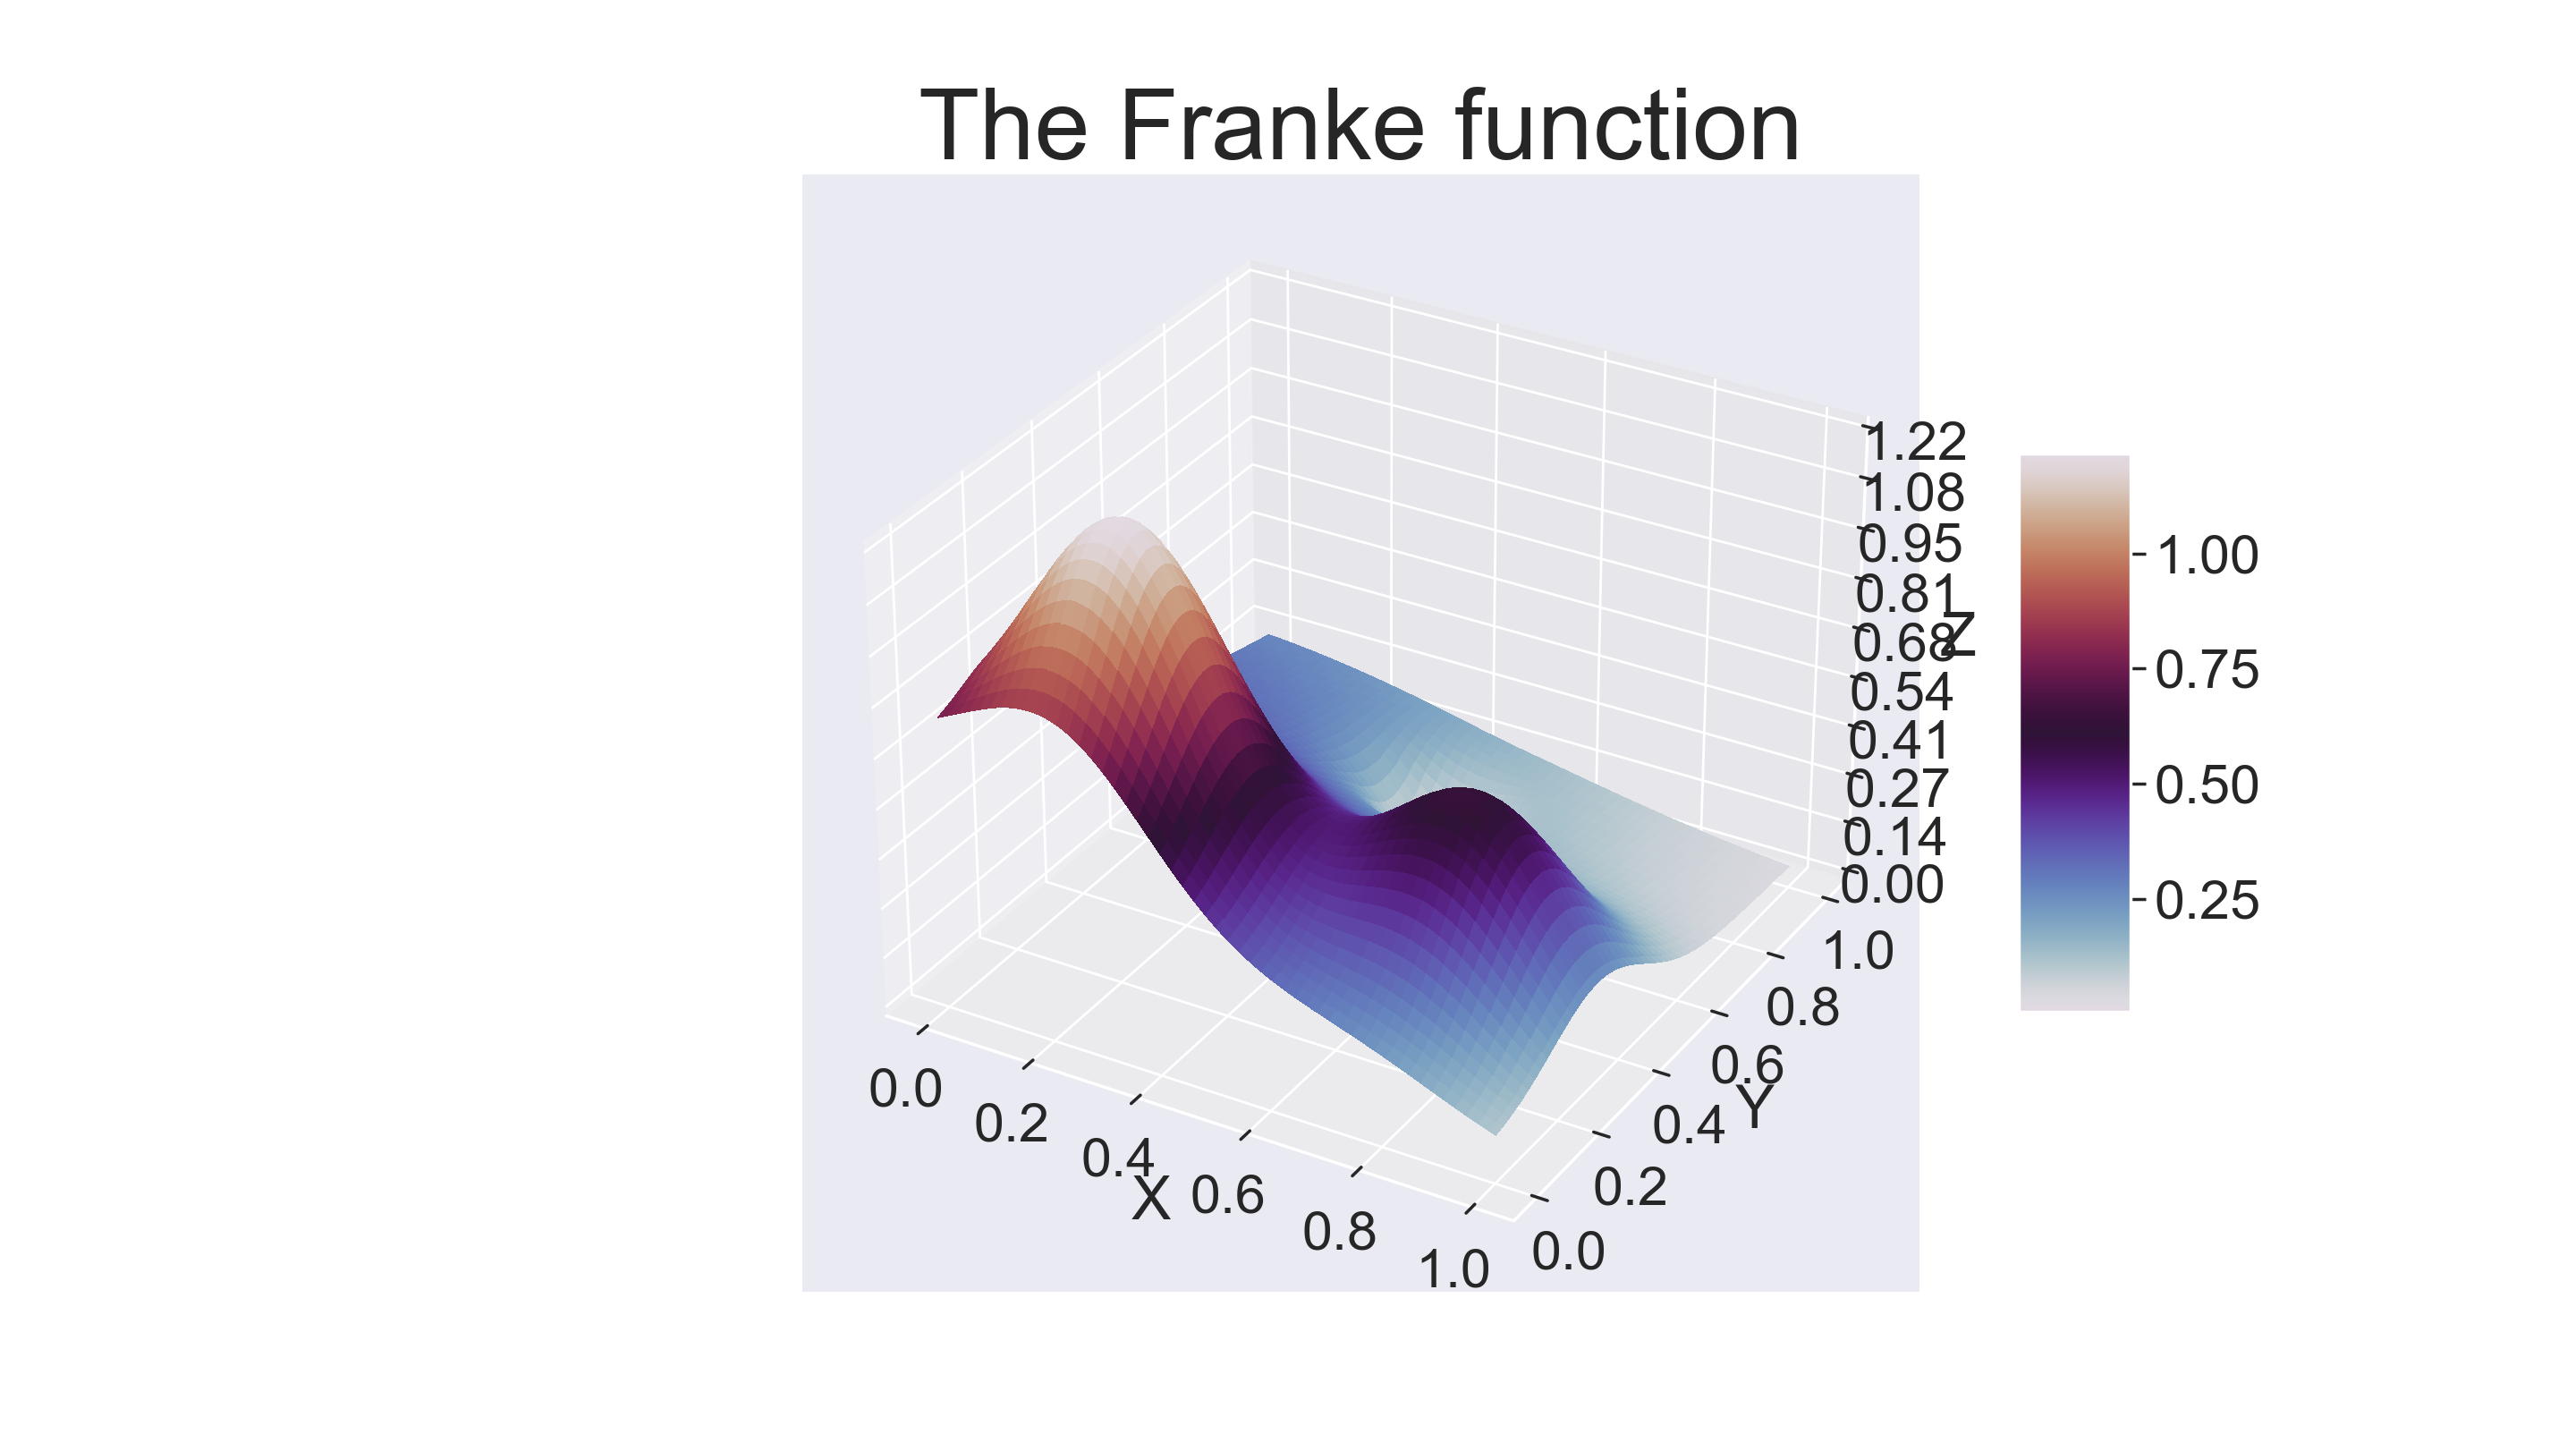
\includegraphics[width=\linewidth]{images/Figure_1.png}
	\caption{\centering A plot of the Franke function }
\end{figure}
%
The number of data points created of the Franke function was a $20 \cross 20$ matrix where $20\%$
of the data set was set aside as testing data while the remaining $80\%$ was used for training. The noise was reduced from $\mathcal{N}(0,1)$ as proposed in the project description, to $\mathcal{N}(0,0.1)$ for better results.

\subsubsection{OLS}
\noindent First the data was fitted with the OLS method, where varying degrees of polynomials was used to create the design matrix. Since the design matrix in this case was non-invertible, singular value decomposition was used to find the $\beta$-values needed to create a model. After the regression was done, the mean square error and the R2 score was calculated for both the testing and training data sets. The different coefficients and $\beta$ values was plotted for polynomial degrees in range $0-5$. The result for this analysis of the Franke function is shown in figures \eqref{MSE and R2 OLS}, \eqref{MSE and R2 OLS noise} and \eqref{beta OLS}.

\noindent Next the bootstrap method was implemented with 100 iterations to see how this 
affected the result of the OLS regression analysis. This method was implemented after the data set was split into a train and test set, to keep test data separate when finding $\beta$ values. After re-sampling the training data, the model was trained. Mean square error was calculated for each training and prediction, in addition to the bias and variance, for polynomial degree $0-15$. The error of the training data was plotted against the error of test data, and the error of test was plotted against the bias and variance of the model. 

\subsubsection{Ridge}
\noindent Next Ridge regression was used on the Franke function,
to see if this methods has a better fit than what was obtained with OLS.
Different values for $\lambda$ was used to obtain the best fit as possible for each polynomial degree. For Ridge equation \eqref{eq:beta_ridge} was used to calculate the coefficients. The $\lambda$ was put to zero to see if the model became the same as for OLS, lastly the $\beta$ values for different orders of polynomial was used to fit the models. The models was then plotted to see how these varied and compered to those from the OLS regression.

\noindent In the pursuit of assessing the robustness and reliability of Ridge regression models, we employed cross-validation, specifically scrutinizing the impact of varying regularization parameters, denoted as \(\lambda\). The function \texttt{k\_fold}, was developed to execute the k-fold cross-validation technique, accepting the data set and an integer \(k\) as arguments, and subsequently partitioning the data into \(k\) randomized subsets (folds). It returns \(k\) pairs of training and test indices, each representing a distinct division of the data, enabling model evaluation across varied data scenarios. 

\noindent For each value of \(\lambda\), increased with a factor of 10, the Ridge regression model was trained and validated \(k\) times - once per fold. The data was divided into train and test sets. The design matrix was generated from the \(x\) and \(y\) values, using a specified max polynomial degree. The Ridge model, instantiated with the current \(\lambda\), was then fitted with training data, and predictions were made. The Mean Squared Error (MSE) between the predictions and actual test values was computed and stored in a scores array. The MSE values were averaged per \(\lambda\), providing an unbiased performance metric, and facilitating the analysis and visualization of how distinct regularization parameters influenced model performance. 

\subsubsection{LASSO}
\noindent The LASSO regression equation doesn't result in a straightforward analytical solution like Ridge regression or ordinary least squares. Sci-kit learn was used to help in these computations, and the LASSO regression function was implemented from it's linear regression package. 
%
\noindent Next, cross validation was applied to LASSO regression using the same method as employed for Ridge regression.

\subsection{Real terrain data}
\noindent In the last part of this project real terrain data was analysed. Due to the massive size of the terrain data only the first $500 \cdot 500$ matrix as shown in figure \ref{terrain_data} was used to avoid problems with computer memory. For LASSO we had to use a $20 \cdot 20$ data matrix to be able to run the code in a acceptable amount of time. 
\begin{figure}[H]
	\centering
	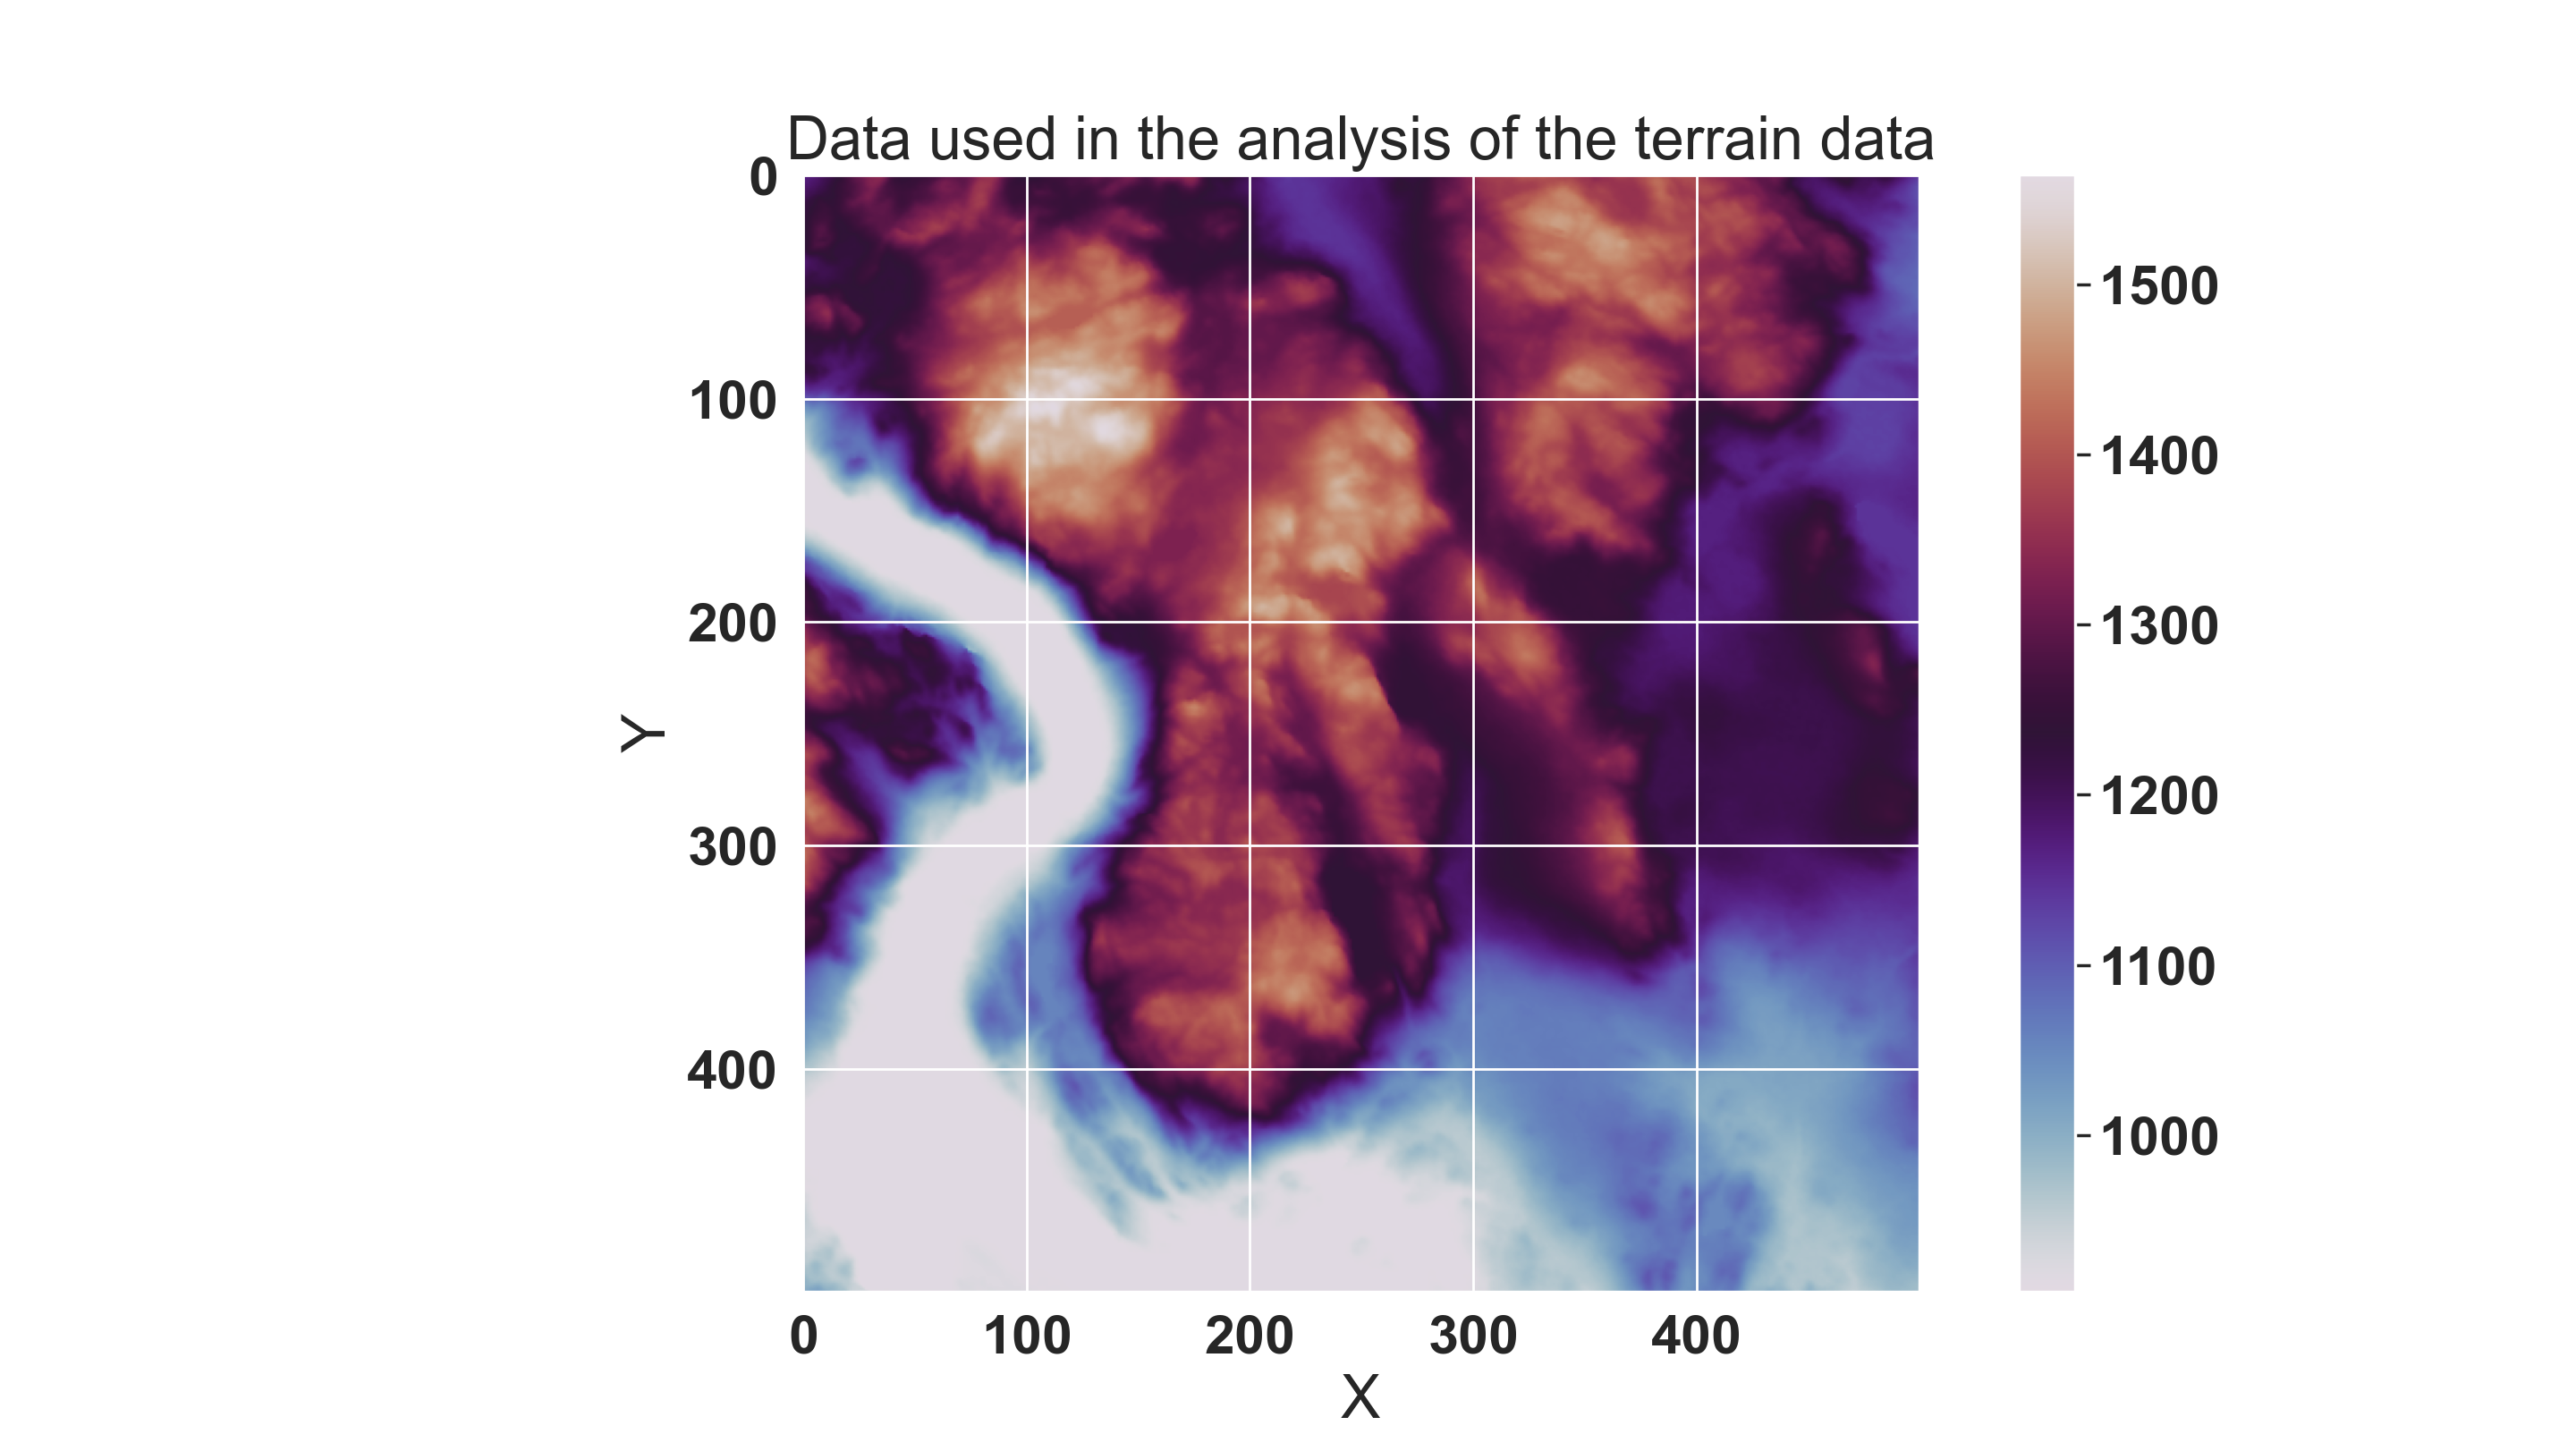
\includegraphics[width=\linewidth]{images/Figure_11.png}
	\caption{A plot of the data matrix used in the analysis of the terrain data in the second part of project 1.}
    \label{terrain_data}
\end{figure}
The data was also scaled by first subtracting the mean value from each column and then divide on the standard deviation so that the variation in height in our data set would not lead to huge MSE values. The OLS regression was applied to create a model of the data set fitted with polynomials of degree $0-10$. The same was done for Ridge, but here also a heat map of the MSE as a function of both different $\lambda$ values and complexity was created. The same was done for LASSO but here as mentioned above one had to downsize the data set to a $20 \cdot 20$ matrix when running over different $\lambda$ values, for the calculation of MSE and R2 score as a function of complexity the normal size data was used ($500 \cdot 500$ matrix).
%
\section{Results}
\thispagestyle{plain}
\subsection{Franke function}
\subsubsection{OLS}
\noindent Our initial step involved the application of OLS to the Franke function without noise.	
This analysis was conducted without employing any resampling techniques, 
and our data set consisted of $20 \cdot 20$ data points. The results for the MSE and R2 score is shown in 
figure \eqref{MSE and R2 OLS}
%
\begin{figure}[H]
	\centering
	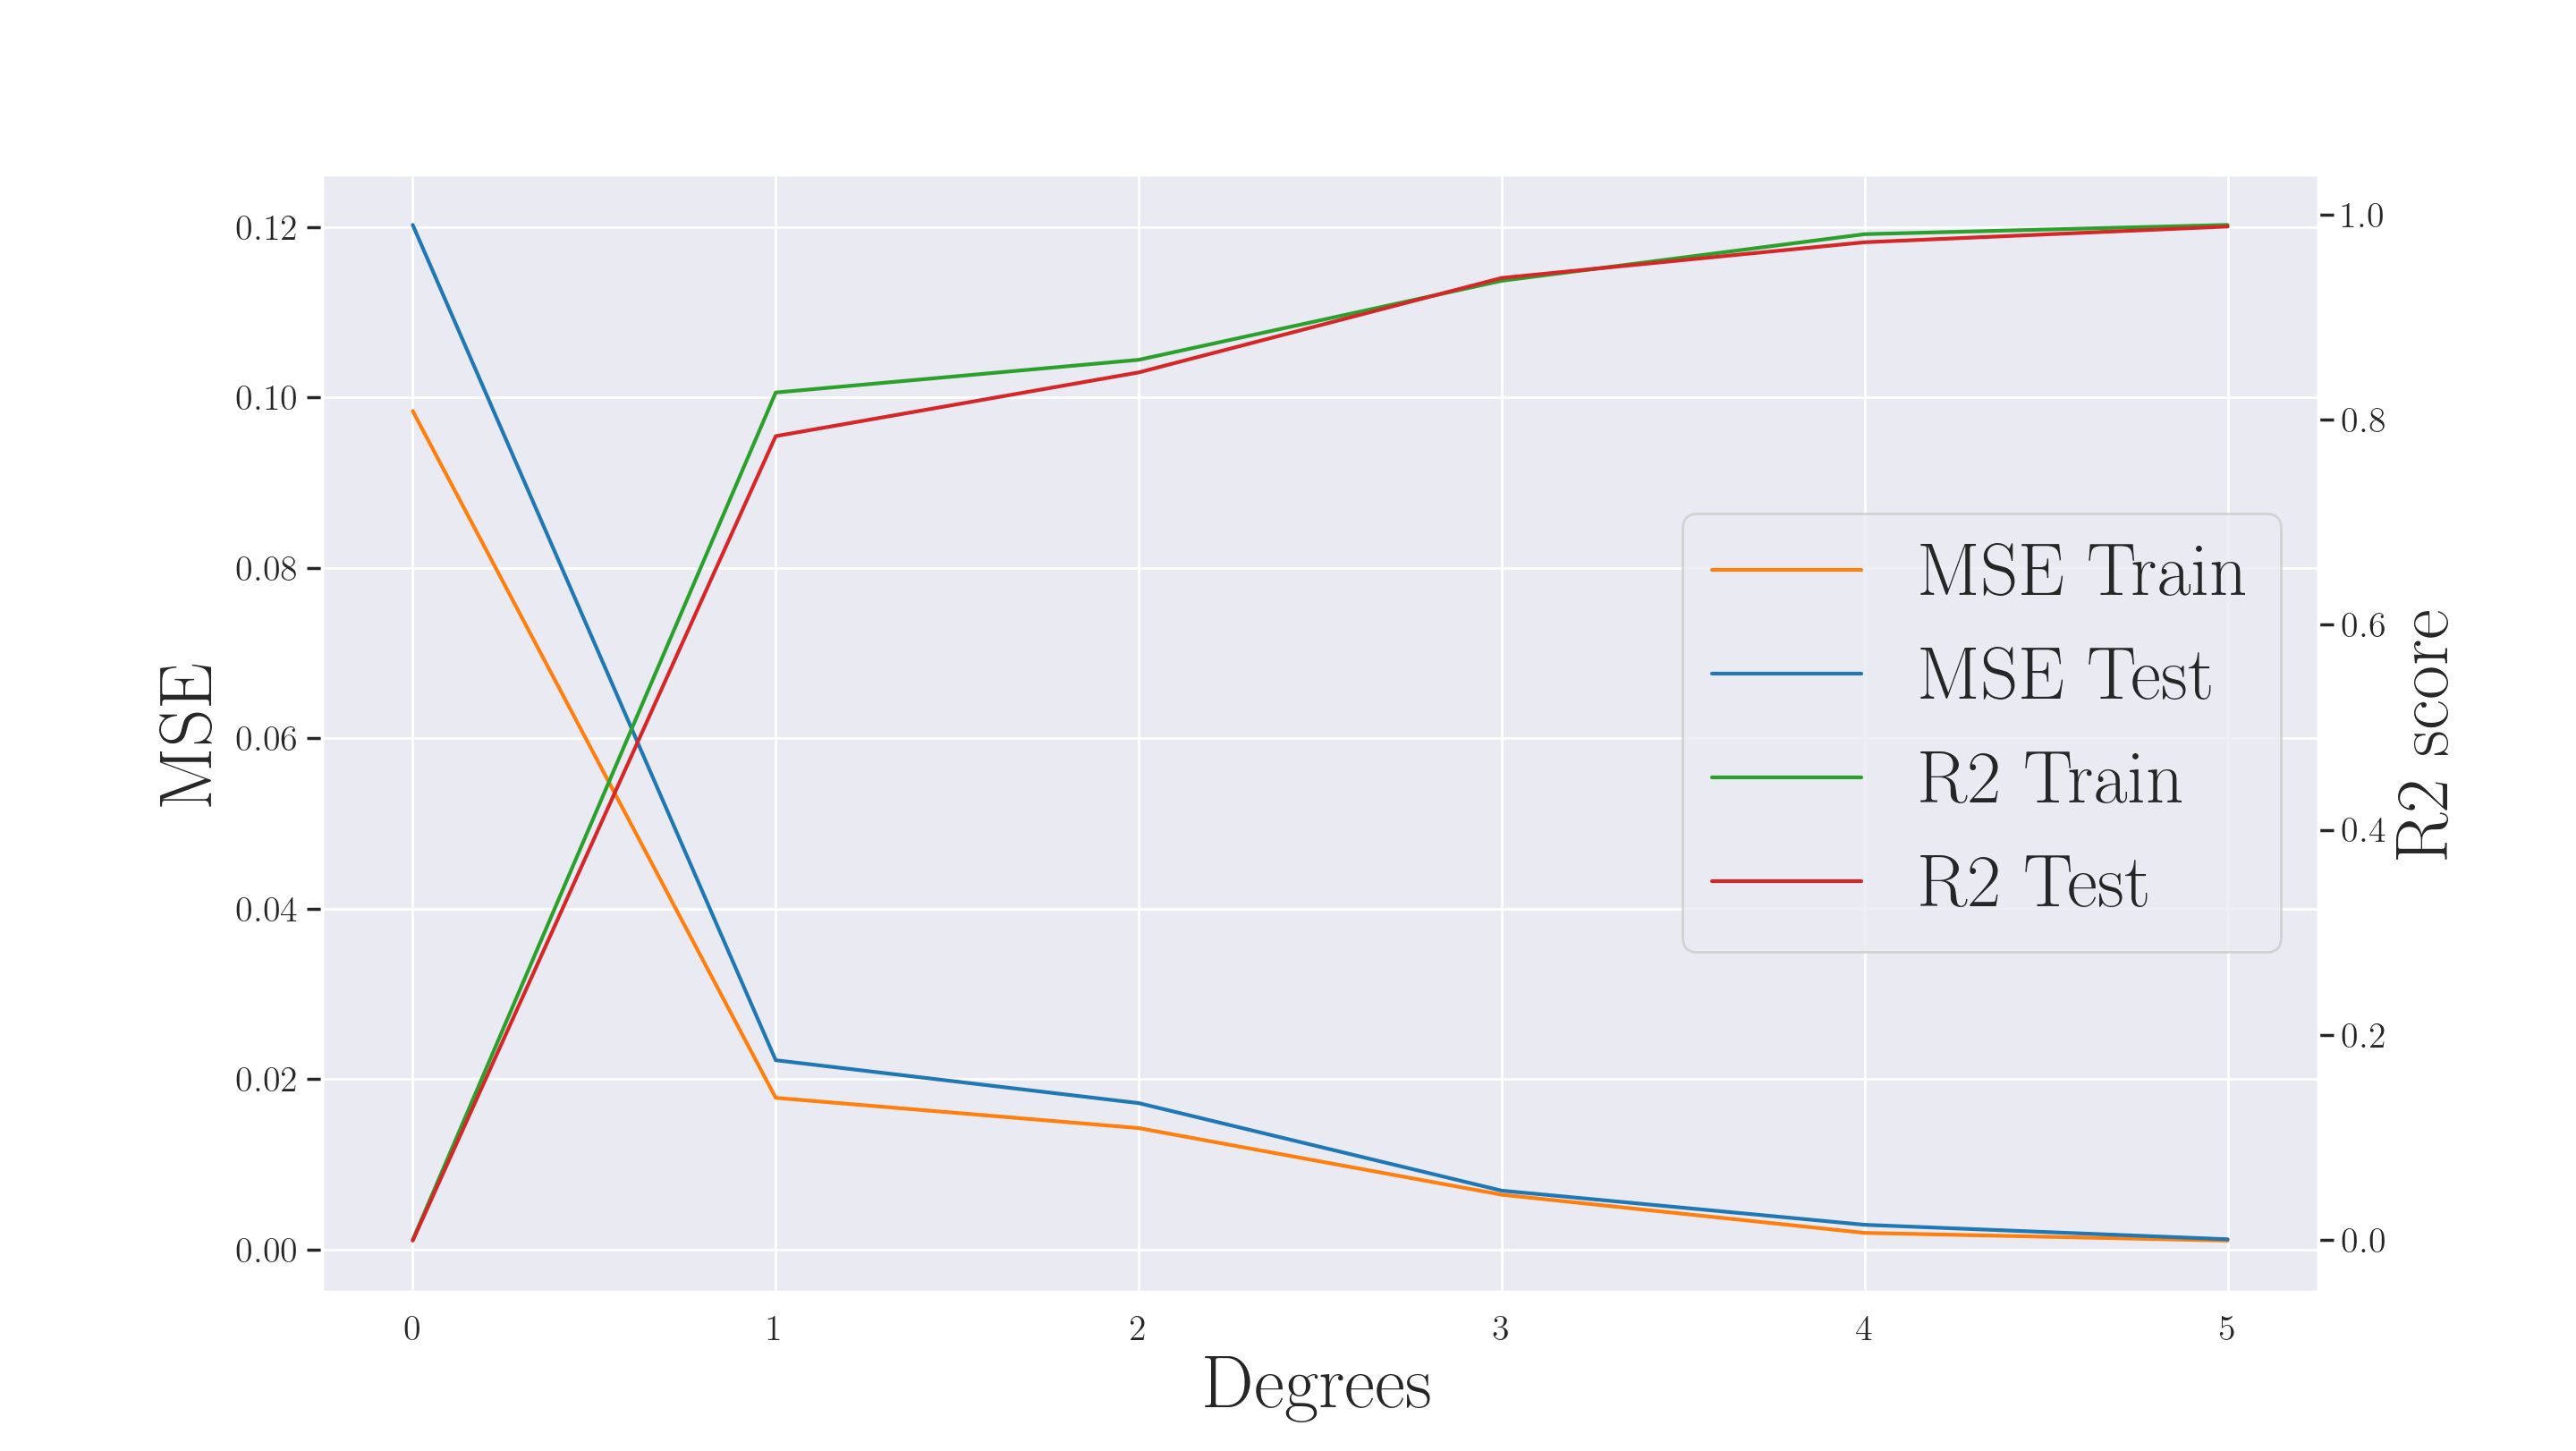
\includegraphics[width=\linewidth]{images/Figure_3.png}
	\caption{Plot showing the MSE and R2 score for the Franke function without noise. The regression method used was OLS.}
	\label{MSE and R2 OLS}
\end{figure}
\noindent The next step was to include noise given by the normal distribution $\mathcal{N}(0,0.1)$. Figure \eqref{MSE and R2 OLS noise} shows how the MSE and R2 score changes when noise is included in to the data set.
\begin{figure}[H]
	\centering
	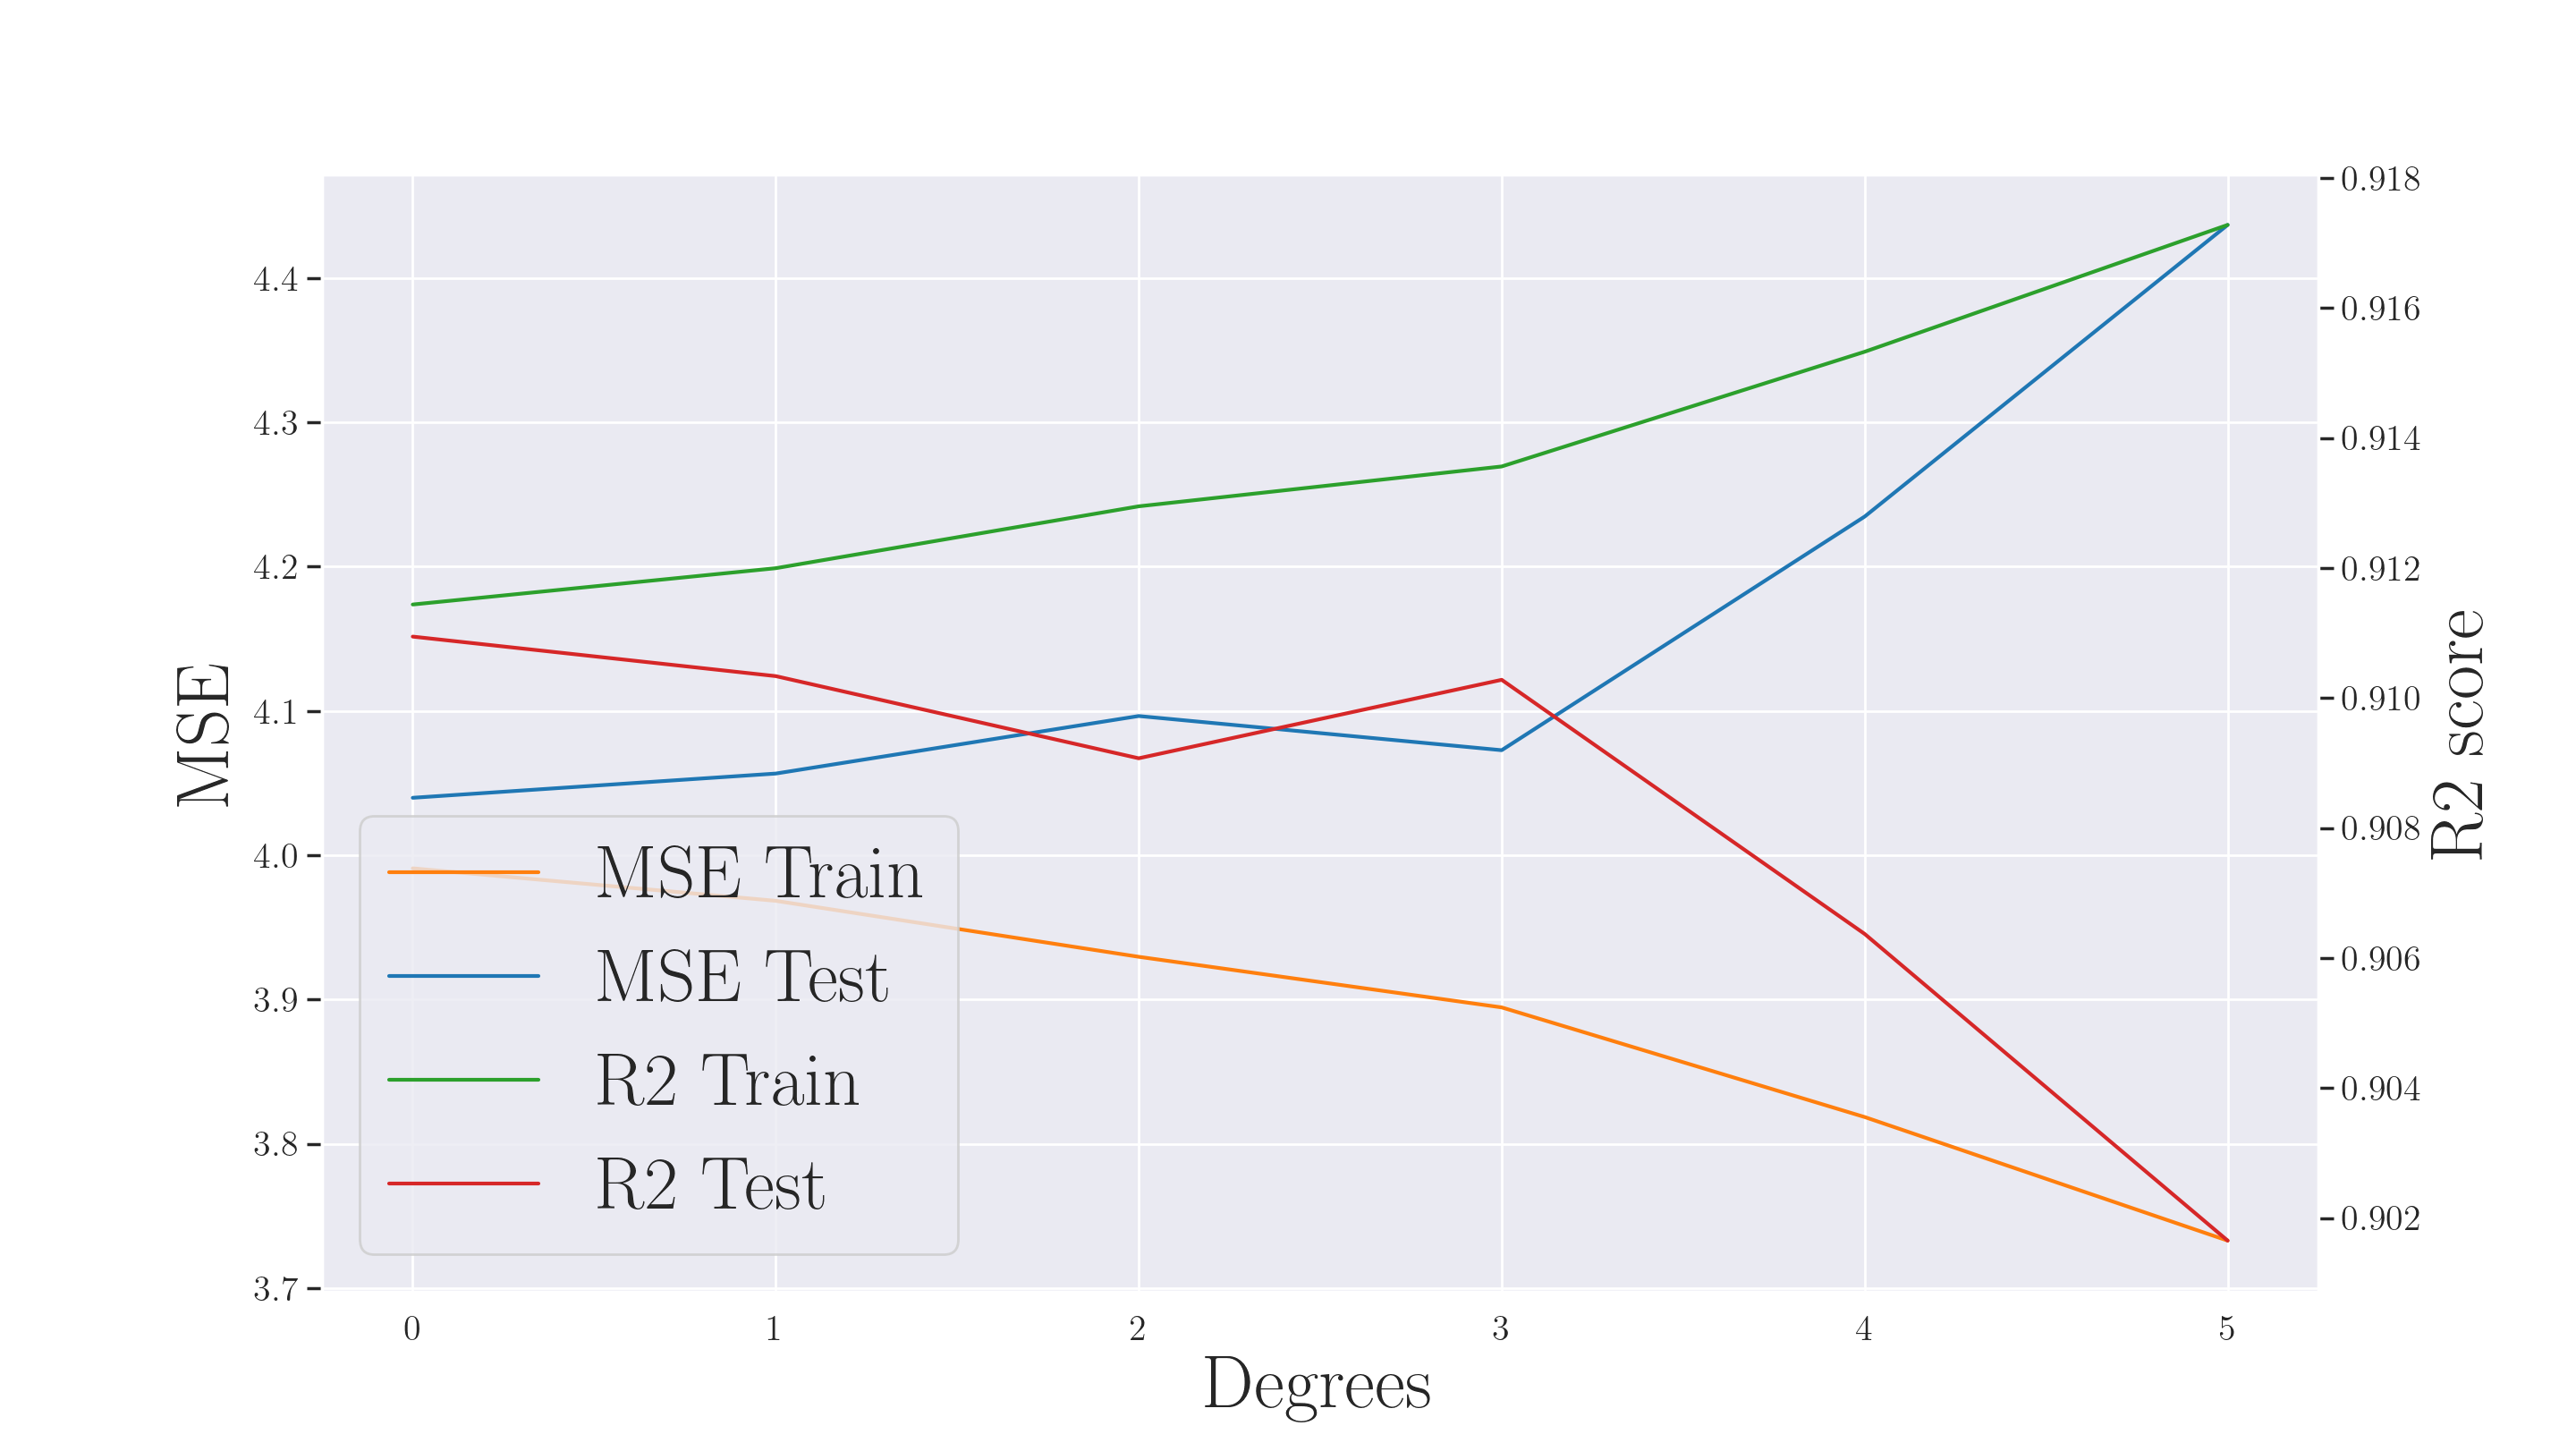
\includegraphics[width=\linewidth]{images/Figure_4.png}
	\caption{Plot showing the MSE and R2 score for the Franke function with noise $\mathcal{N}(0,0.1)$. The regression method used was OLS.}
	\label{MSE and R2 OLS noise}
\end{figure}
\noindent We then plotted the coefficients for the different orders of polynomials to see how these varies in value.
\begin{figure}[H]
	\centering
	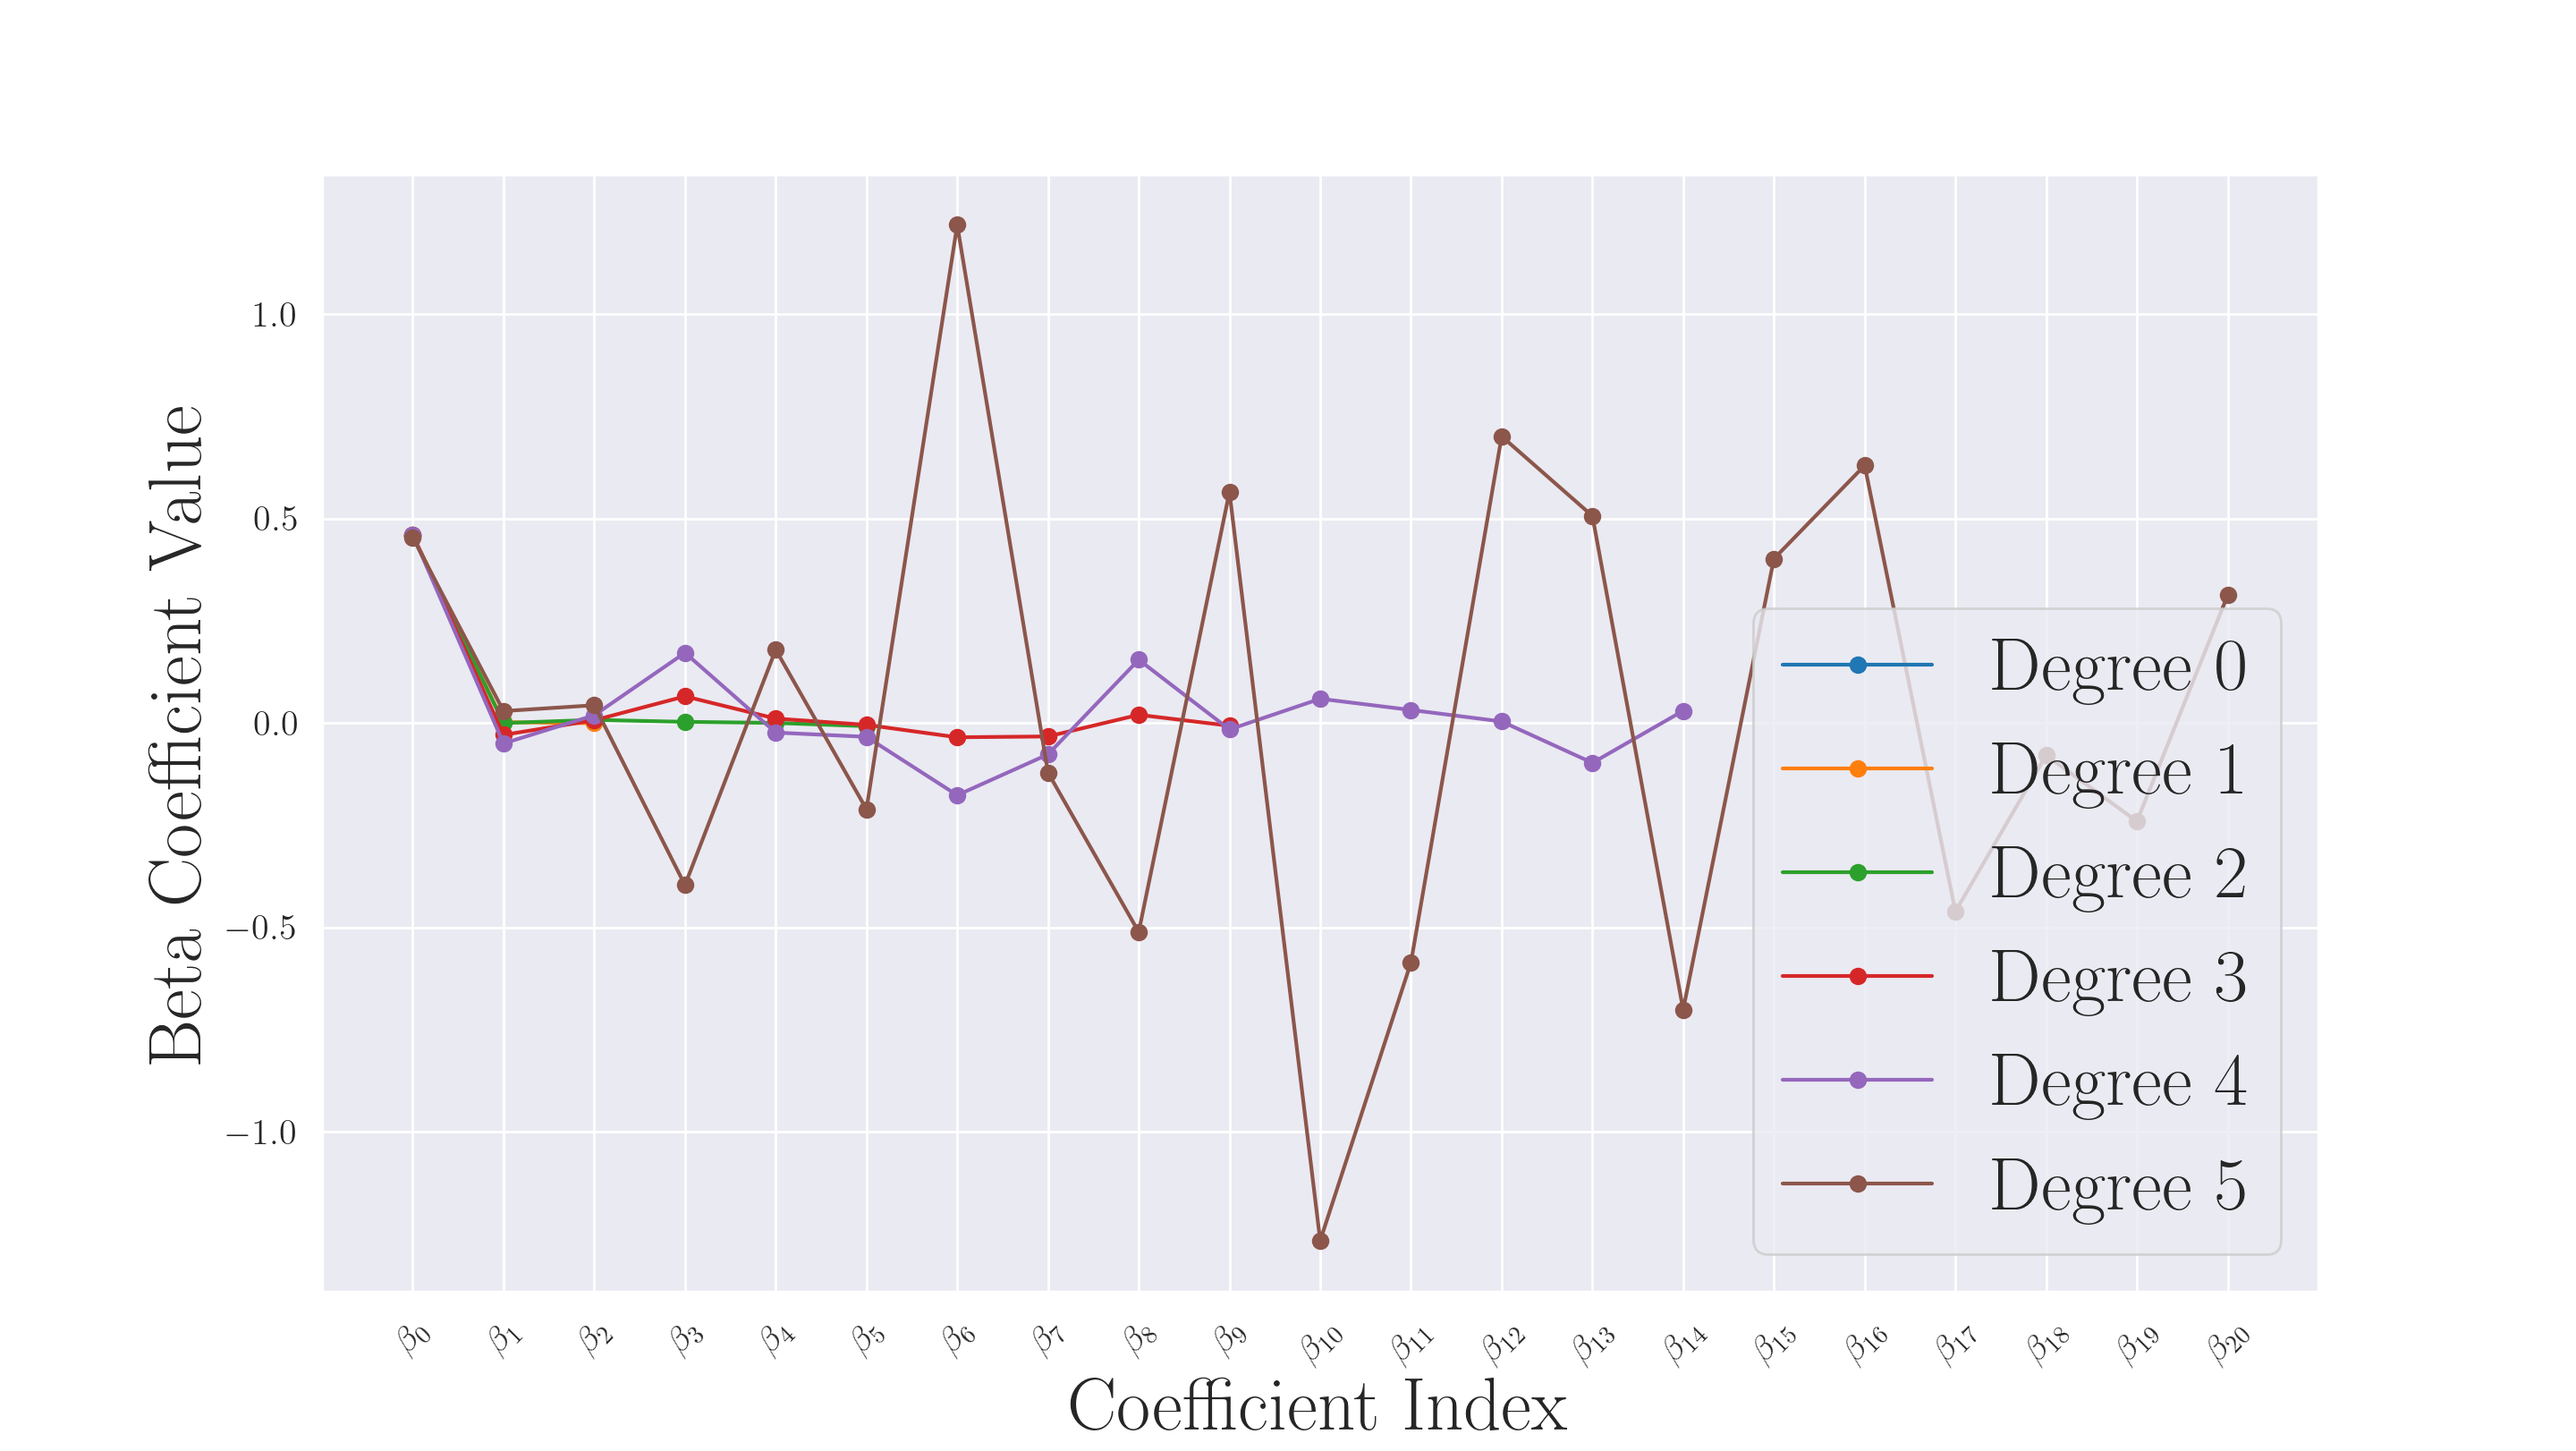
\includegraphics[width=\linewidth]{images/Figure_12.png}
	\caption{A plot showing the $\beta$ values for OLS for different orders of polynomials.}
	\label{beta OLS}
\end{figure}
%
\noindent Figure \ref{fig:bootstrap_error} is showing the error of training and test data for polynomial degree $0-15$. There is a consistent reduction in error of training for higher polynomial degree, whereas the error of test increase with polynomial degree $6-15$.
\begin{figure}[H]
	\centering
	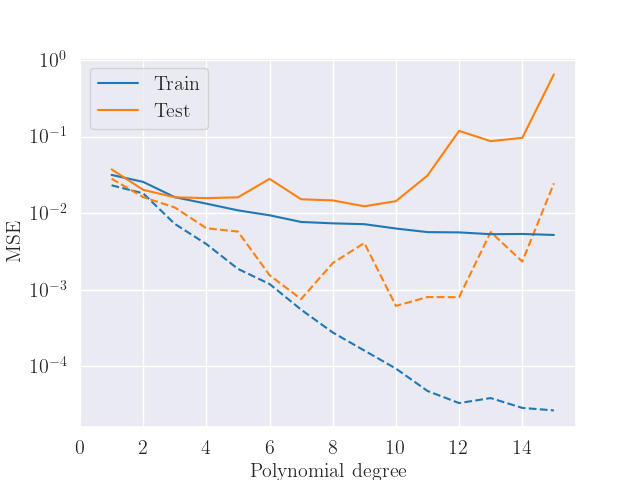
\includegraphics[width=\linewidth]{images/bootstrap_error.png}
	\caption{MSE of the models prediction for polynomial degree $0-15$, using the Franke function. The solid lines describe the MSE where noise is added to the function, dotted lines describe MSE where noise is not added.}
    \label{fig:bootstrap_error}
\end{figure}
%
\noindent Figure \ref{fig:bias_variance} is showing the error of prediction, and the bias and variance of the model for polynomial degree $0-15$. 
% 
\begin{figure}[H]
    \centering
    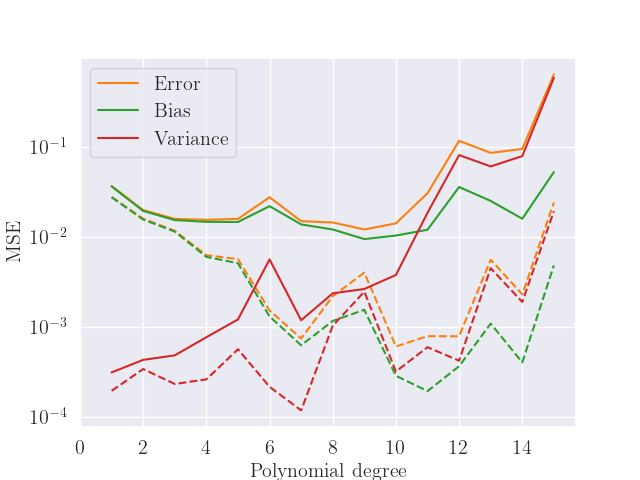
\includegraphics[width=\linewidth]{images/bias_variance.png}
    \caption{MSE of the models predicted error, using the Franke function, bias and variance. The solid lines describe the MSE where noise is added to the function, dotted lines describe MSE where noise is not added.}
    \label{fig:bias_variance}
\end{figure}
\noindent We compared number of folds used when re-sampling data from the Franke funktion without noise, by using OLS as regression method. In figure \ref{fig:cv_kfolds} we plot MSE for each fold $k=[5-10]$, to determine an ideal division of the data available.
\begin{figure}[H]
	\centering
	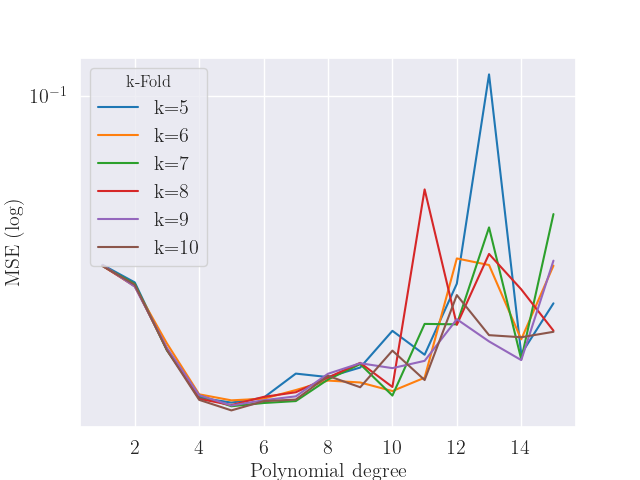
\includegraphics[width=\linewidth]{images/cv_kfolds.png}
	\caption{MSE of prediction error for polynomial degree $0-15$, using the Franke function, with cross validation $k=5-10$.}
 \label{fig:cv_kfolds}
\end{figure}

\subsubsection{Ridge}
\noindent For Ridge regression we started by making a heat map of how the MSE changes as a function of complexity and $\lambda$ values. Here we tested for 1000 different $lambda$ values from $\lambda_0 = 10^{-8}$ to $\lambda_{1000} = 10^{2}$ and for polynomials with degree 1-5. A plot of the heat map for both the training and testing data set is shown in figure \eqref{heatmap training ridge} and \eqref{heatmap test ridge}.
\begin{figure}[h]
	\centering
	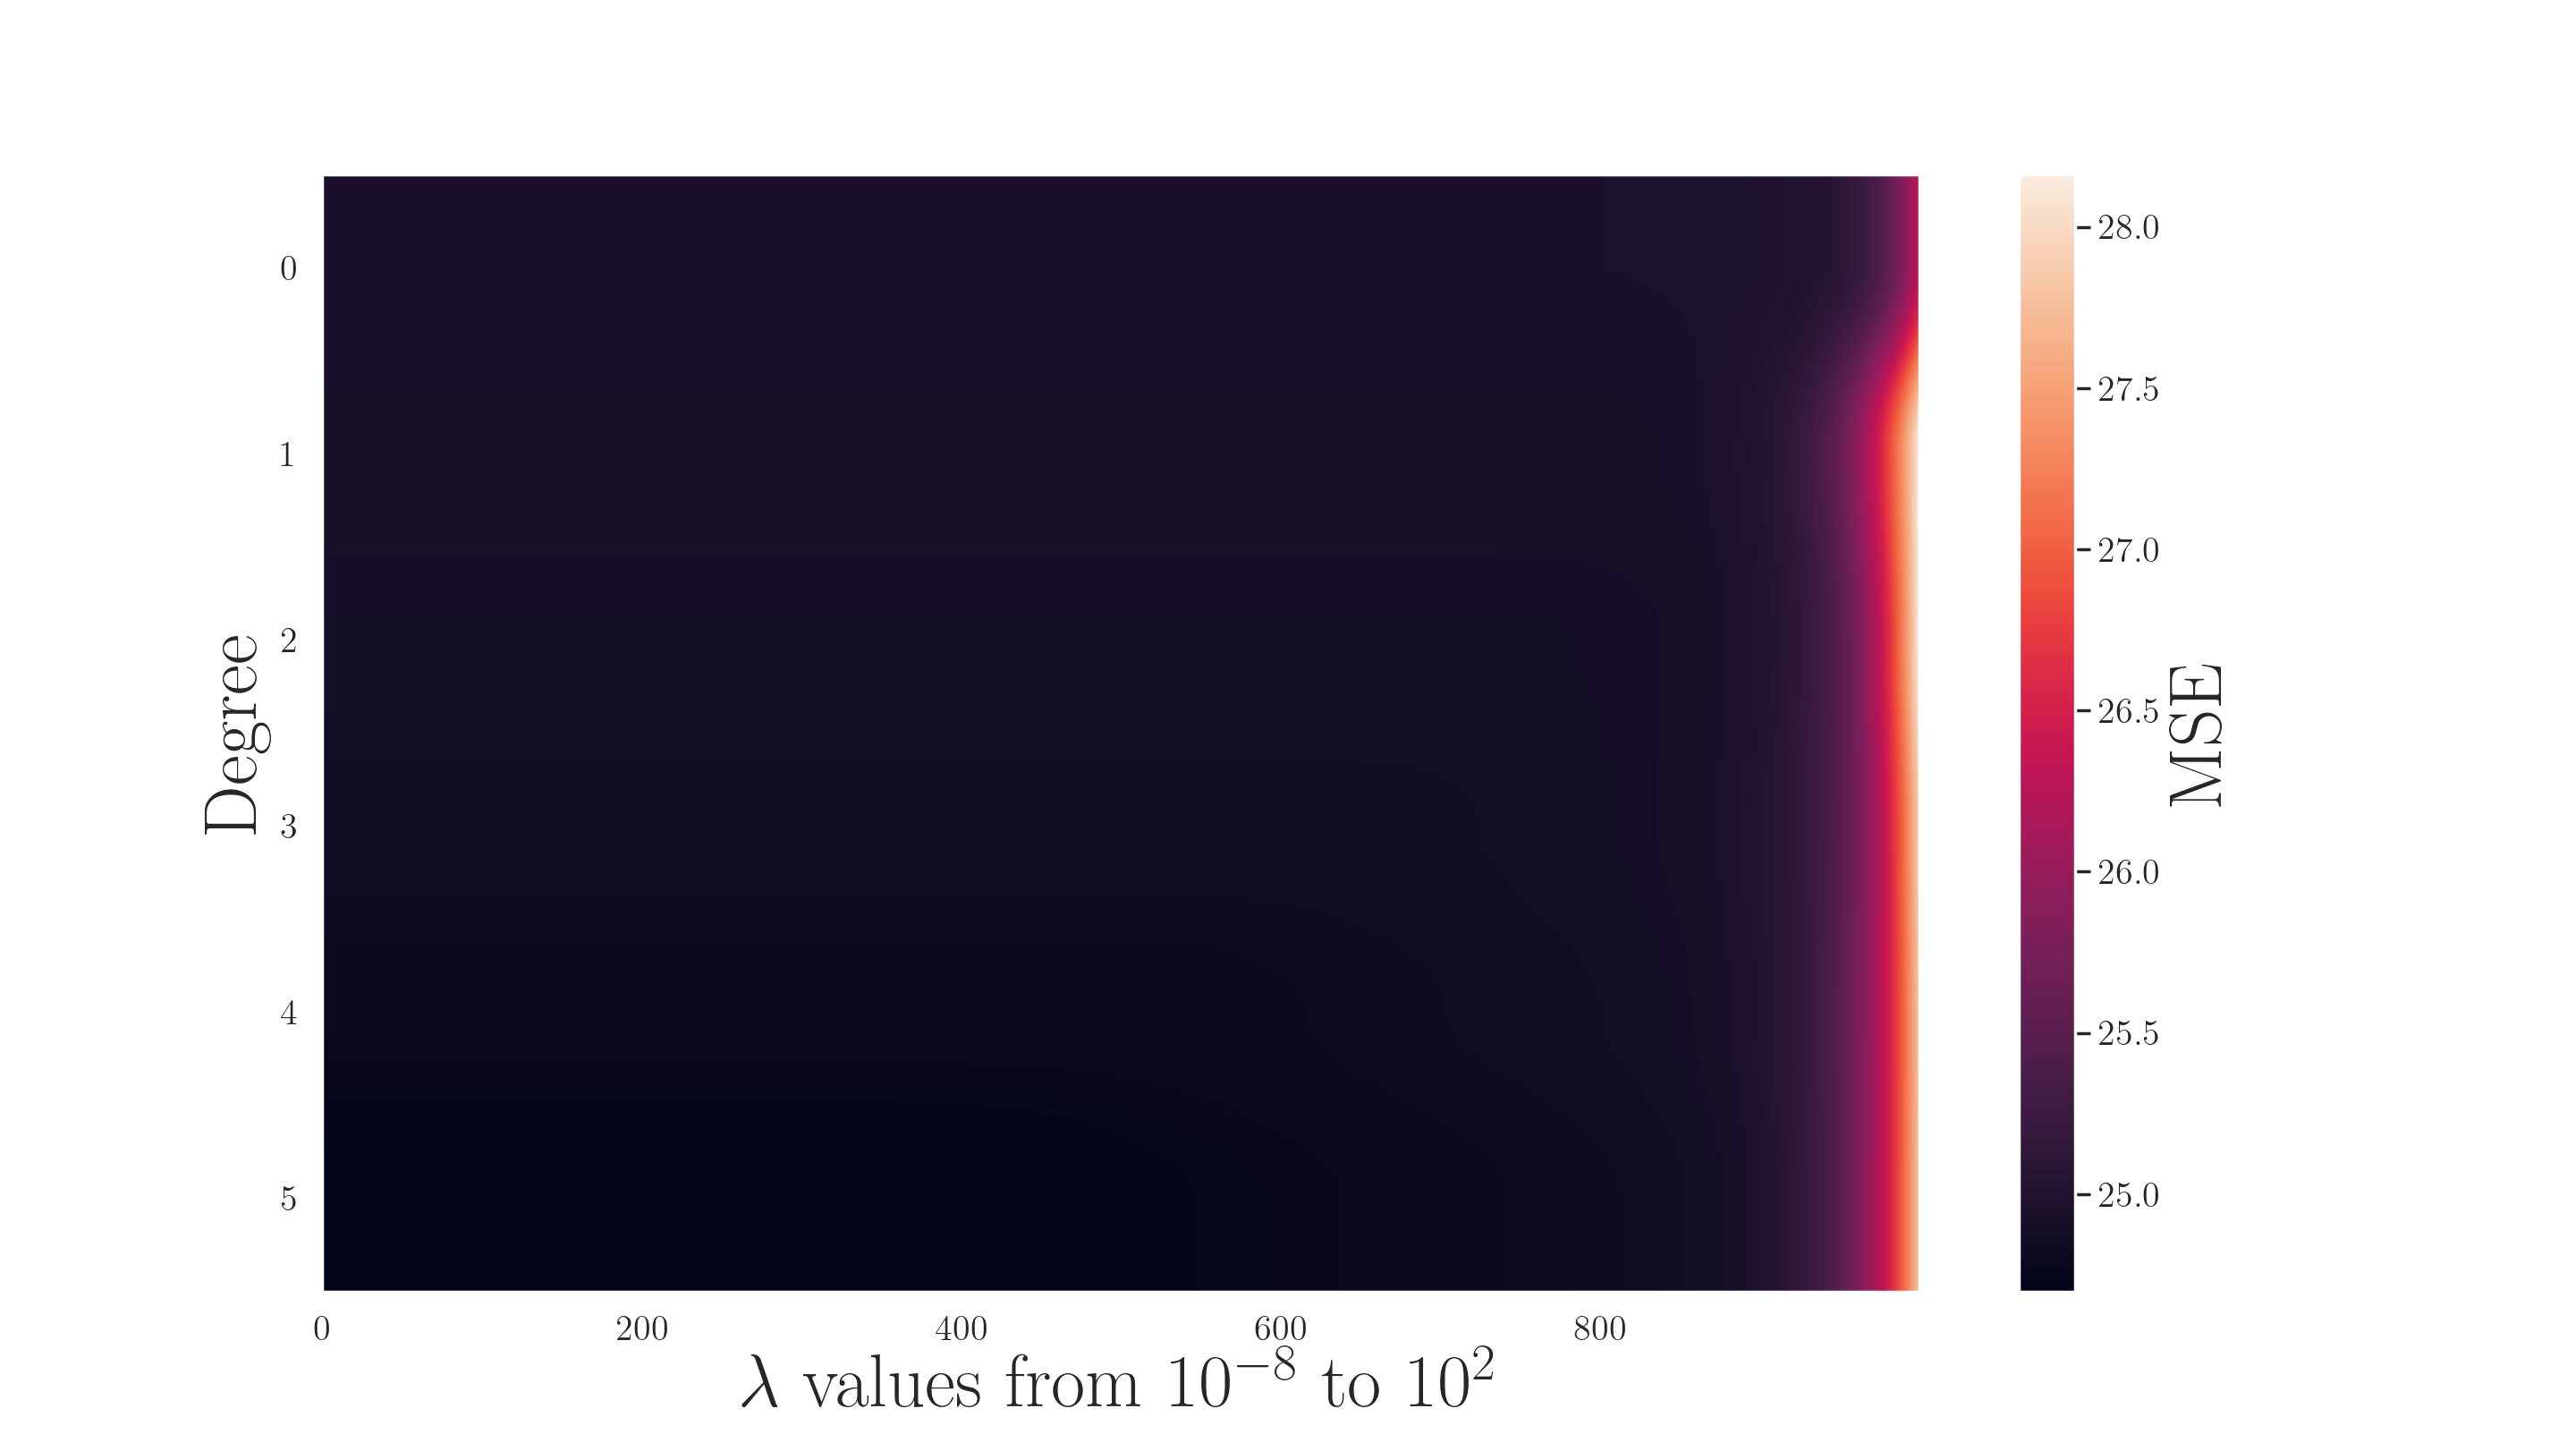
\includegraphics[width=\linewidth]{images/Figure_8.png}
	\caption{A heat map of the MSE for the training data, for different $\lambda$ values and complexities. The $\lambda$ values goes from $10^{-8}$ to $10^{2}$. }
	\label{heatmap training ridge}
\end{figure}
\begin{figure}[H]
	\centering
	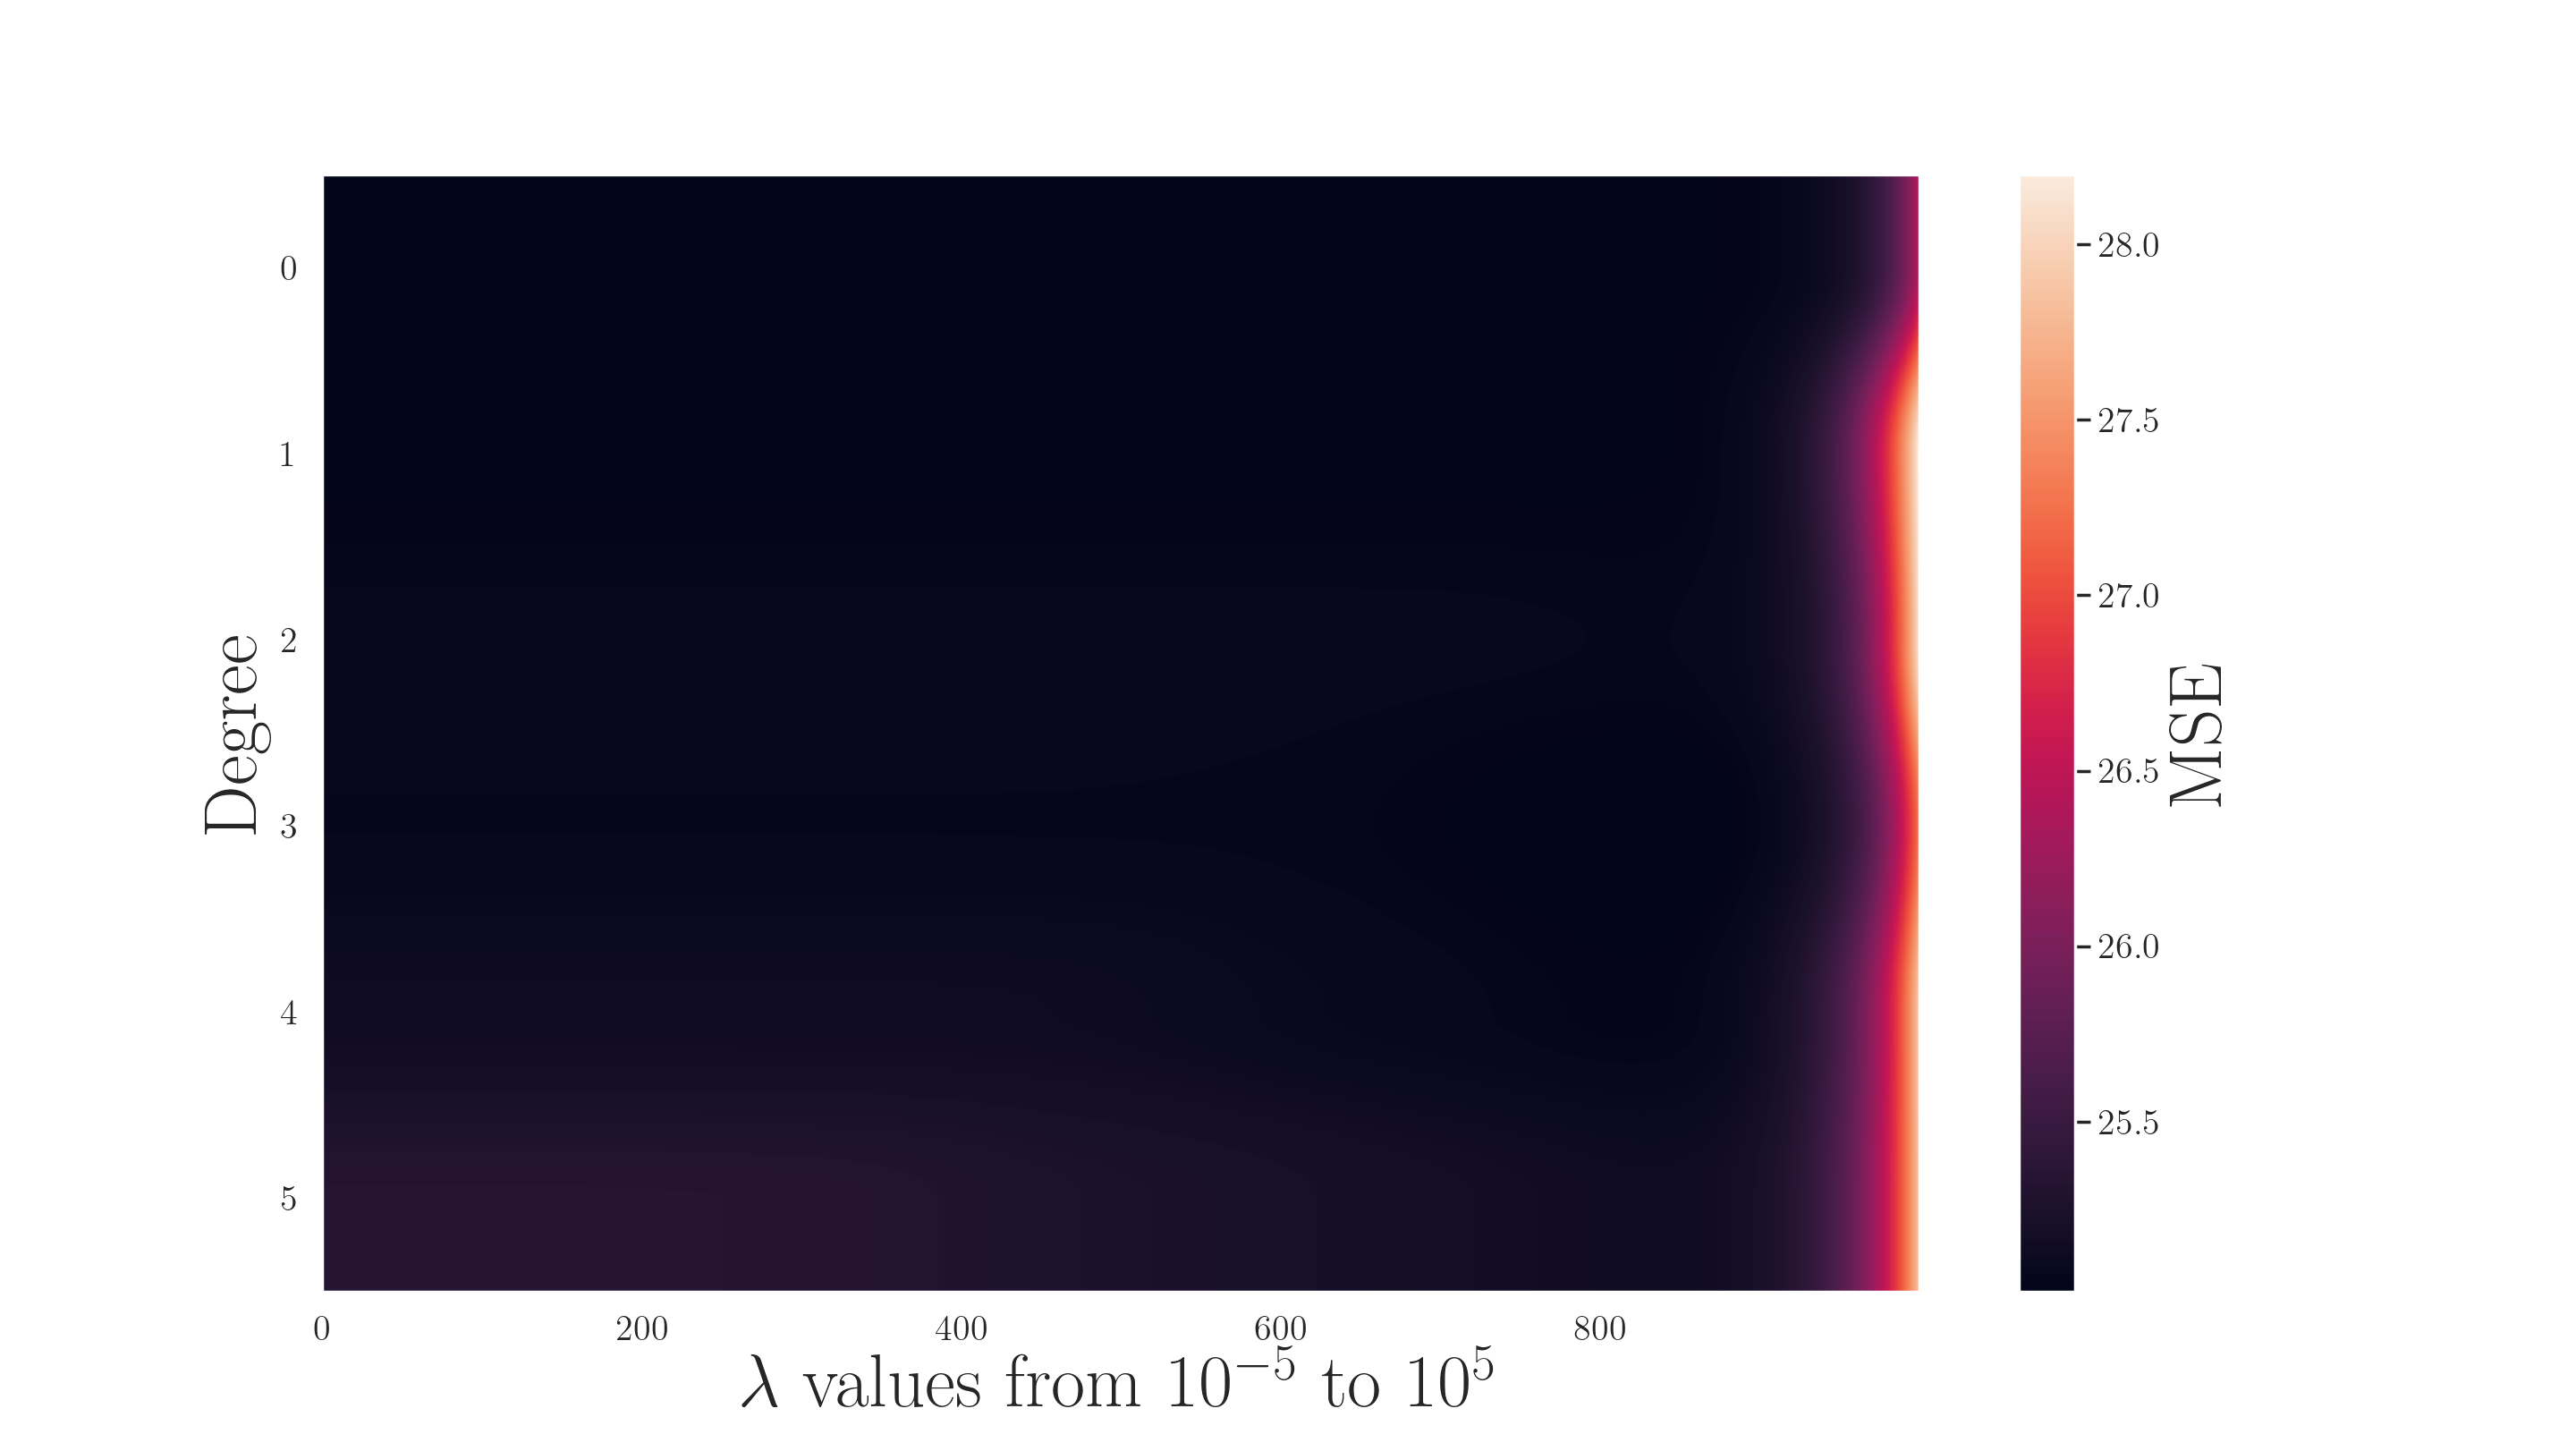
\includegraphics[width=\linewidth]{images/Figure_7.png}
	\caption{A heat map of the MSE for the testing data, for different $\lambda$ values and complexities. The $\lambda$ values goes from $10^{-5}$ to $10^{5}$.}
	\label{heatmap test ridge}
\end{figure}
\noindent Next we used the first $\lambda$ to plot how the MSE and R2 score changes as a function of complexity for the Franke function both with and without noise. Figure \eqref{MSE and R2 Ridge no noise} shows the MSE and R2 score with no noise present in the data set of the Franke function, and figure \eqref{MSE and R2 Ridge noise} shows with noise given by the normal distribution $\mathcal{N}(0,0.1)$.
\begin{figure}[H]
	\centering
	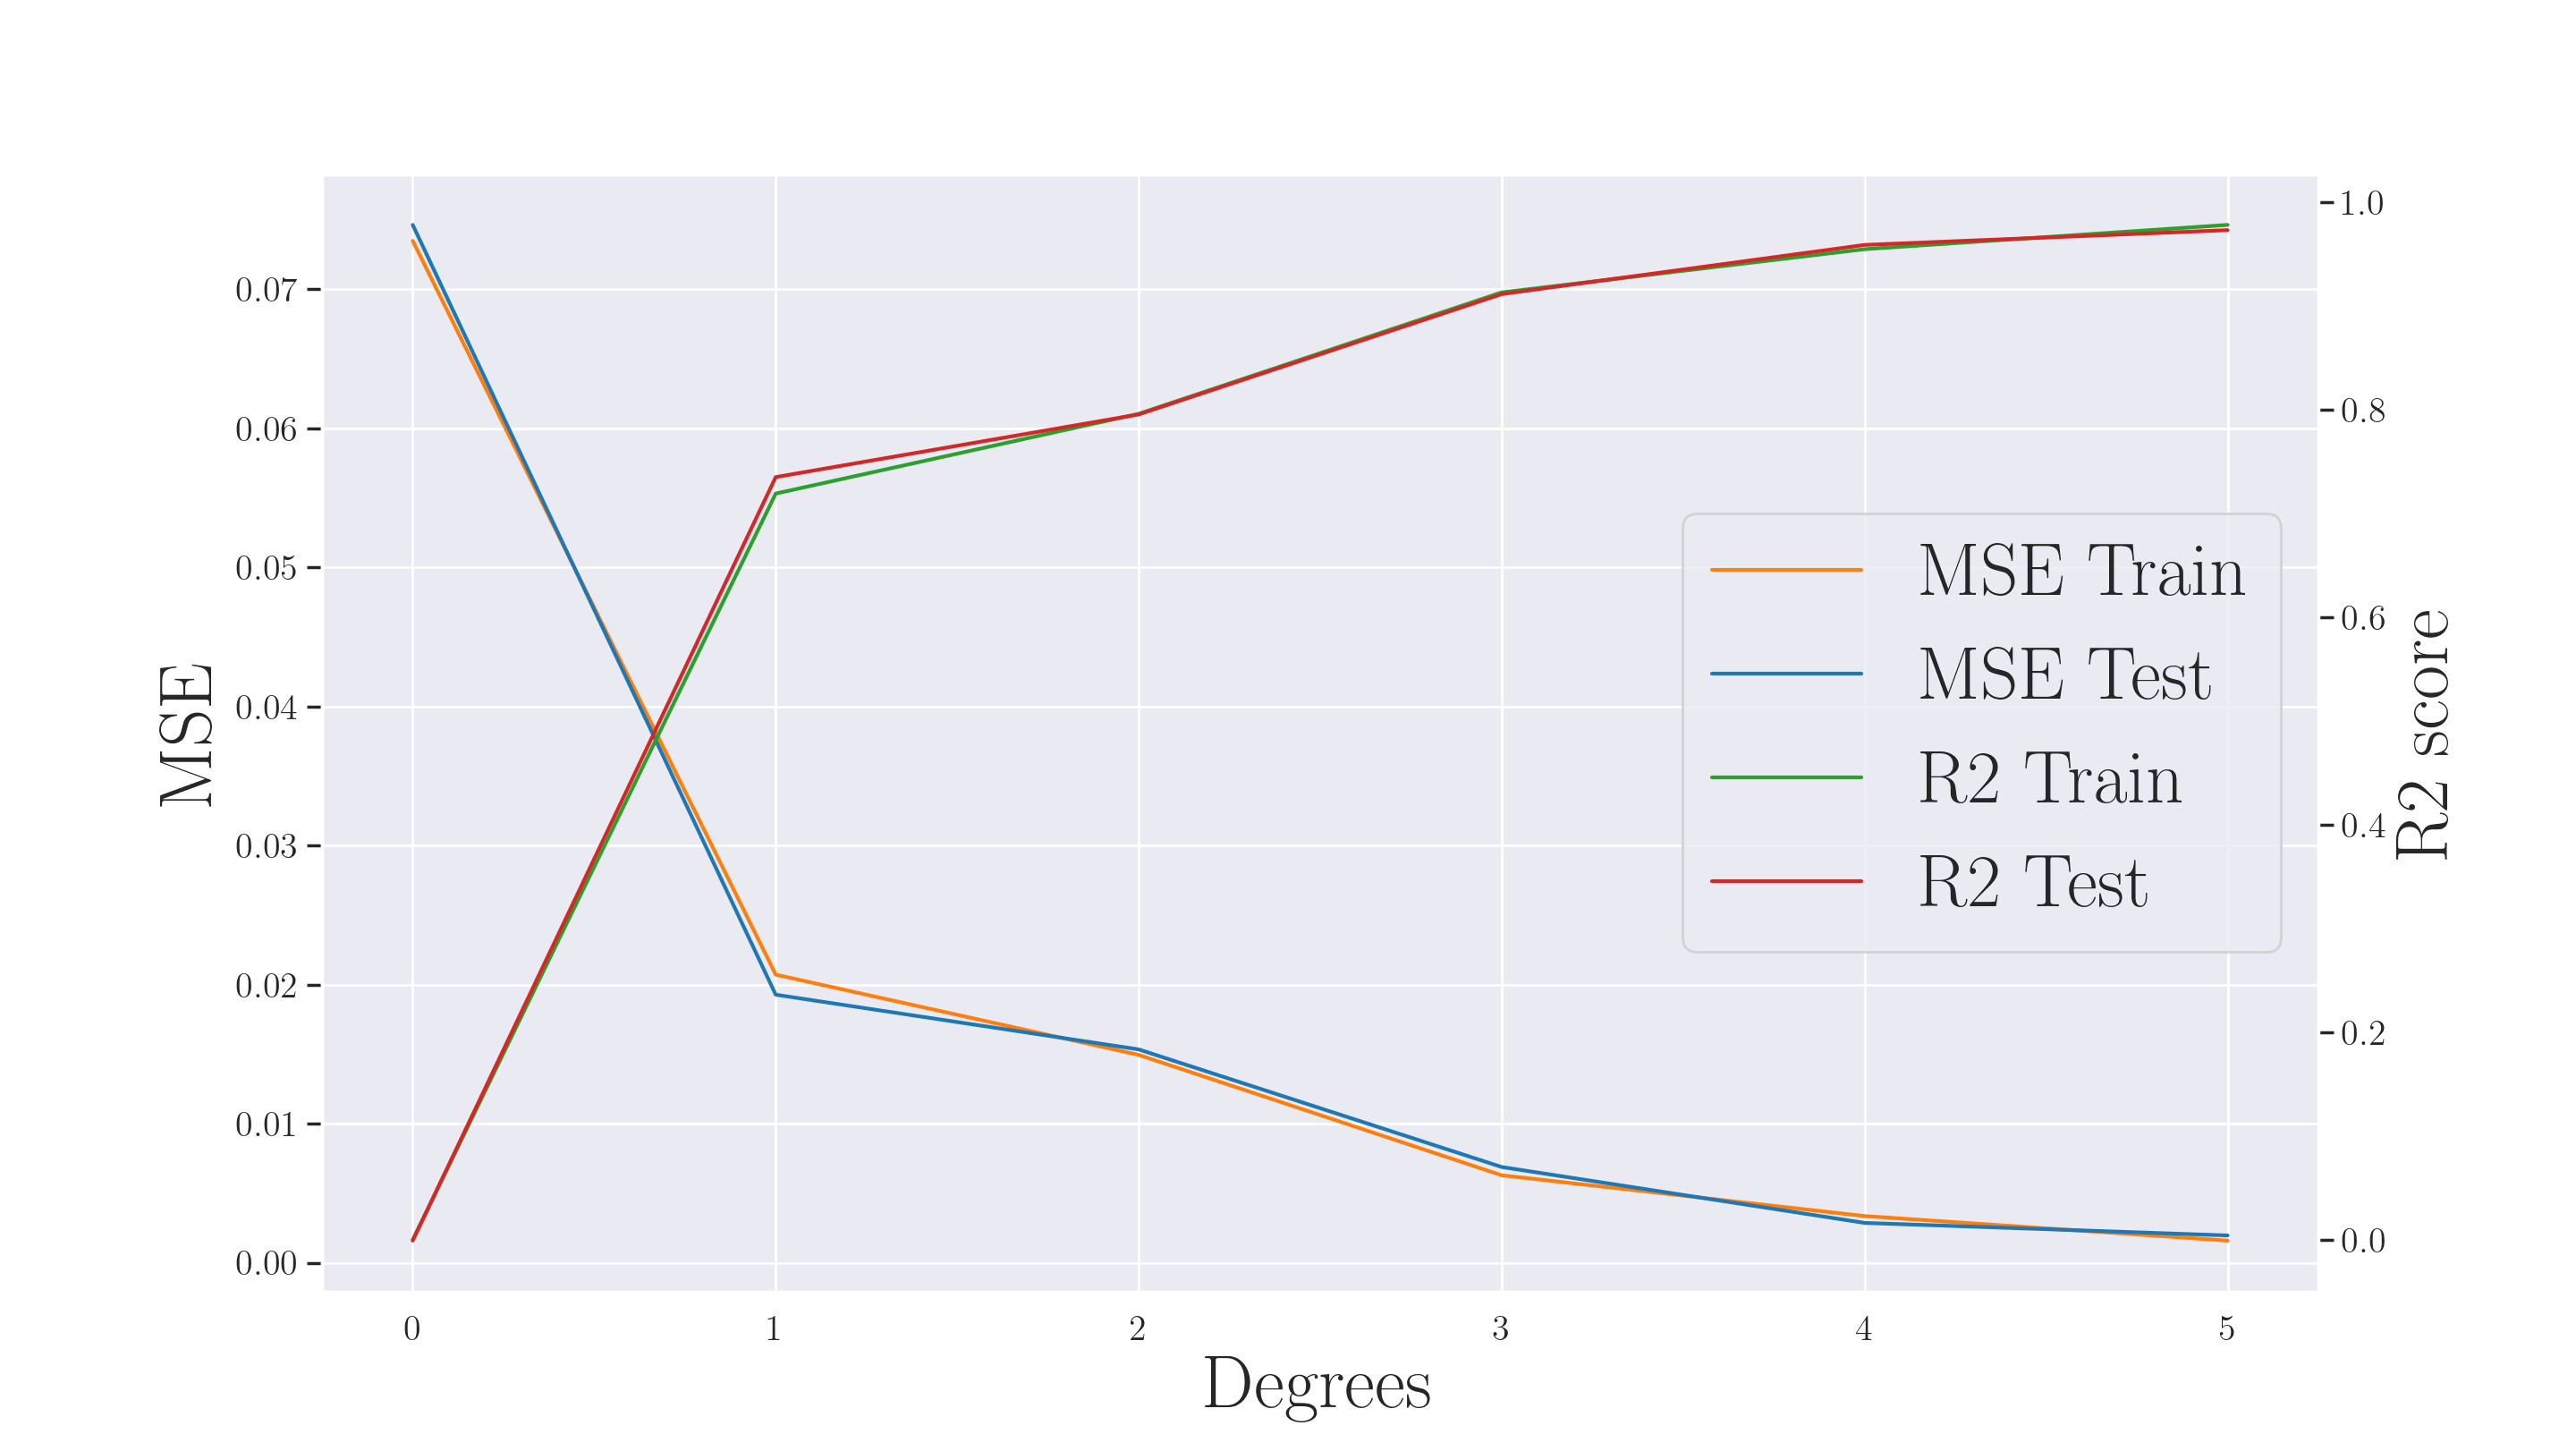
\includegraphics[width=\linewidth]{images/Figure_15.png}
	\caption{A plot of the MSE and R2 score as a function of degrees and a $\lambda$ value of $10^{-5}$ for Ridge regression on the Franke function with no noise present.}
	\label{MSE and R2 Ridge no noise}
\end{figure}
\begin{figure}[H]
	\centering
	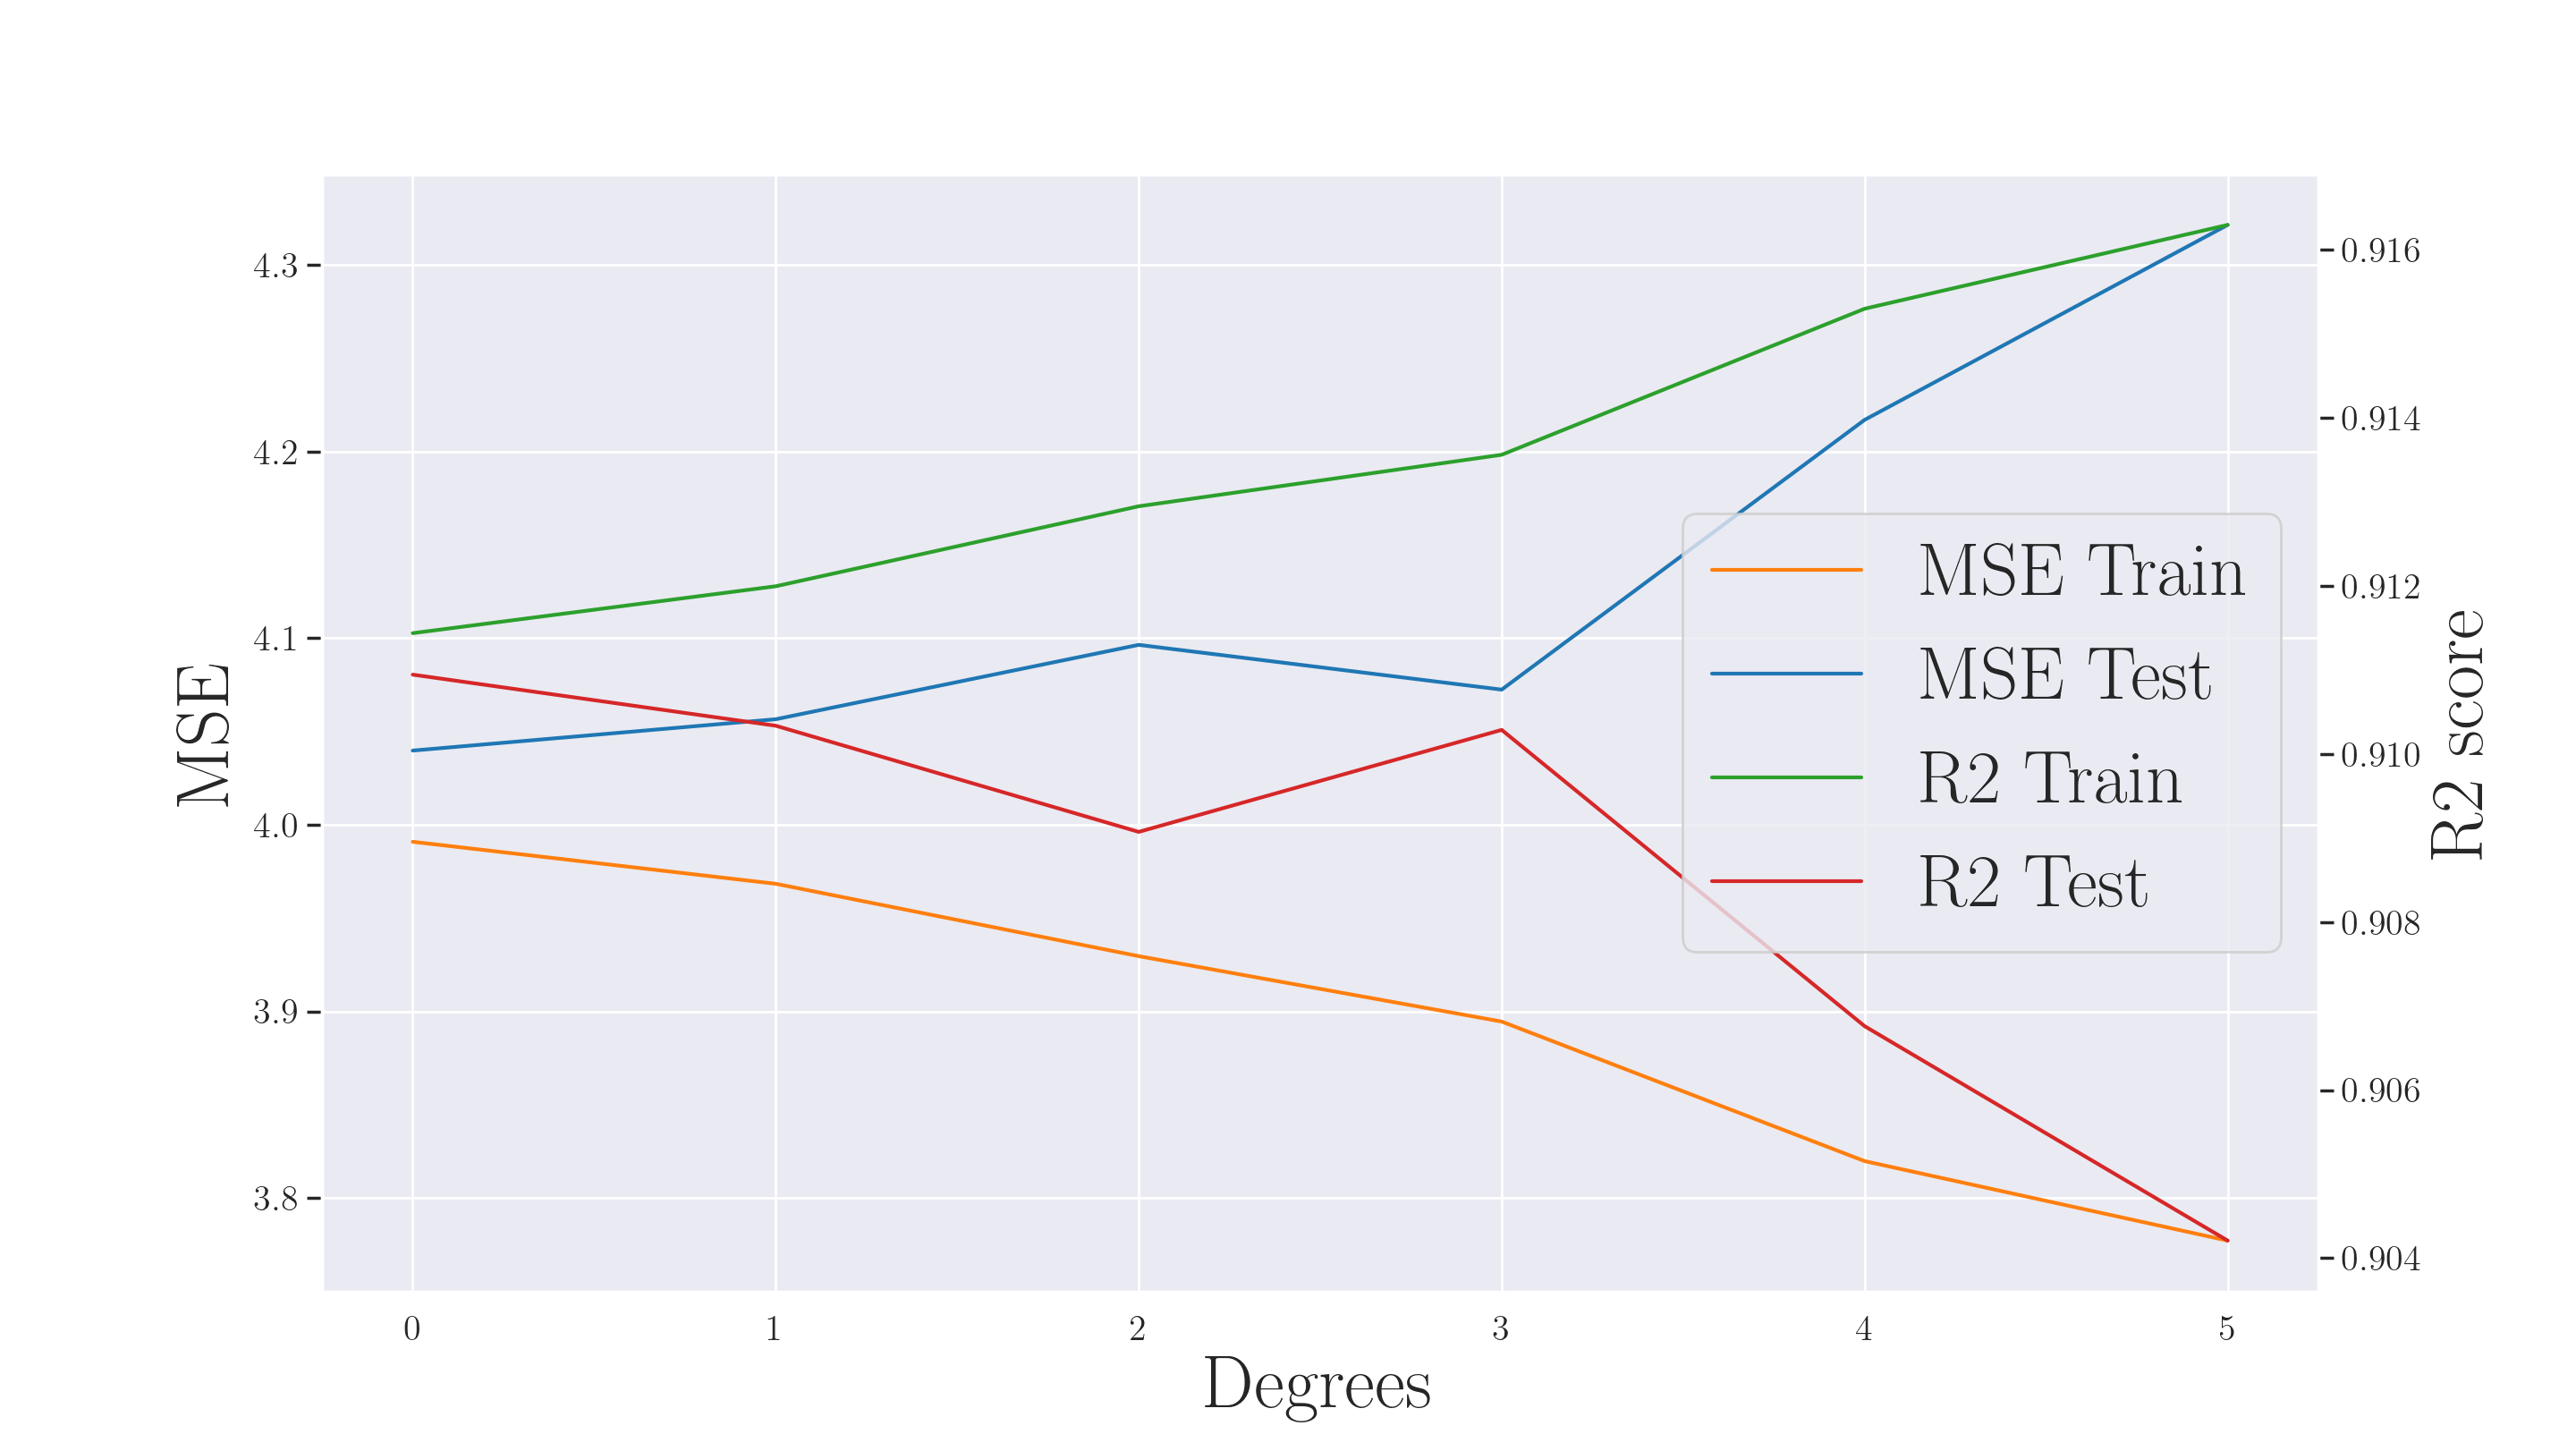
\includegraphics[width=\linewidth]{images/Figure_16.png}
	\caption{A plot of the MSE and R2 score as a function of degrees and a $\lambda$ value of $10^{-5}$ for Ridge regression on the Franke function with noise given by the normal distribution $\mathcal{N}(0,0.1)$.}
	\label{MSE and R2 Ridge noise}
\end{figure}
\noindent We can also see what happens for the ridge regression if $\lambda$ is put to zero. Figure \eqref{MSE and R2 Ridge noise lambda0} shows the MSE and R2 score if $\lambda = 0$, while figure \eqref{Ridge vs OLS} shows the MSE if $\lambda = 0$ and $\lambda = 10^{-5}$. 
\begin{figure}[H]
	\centering
	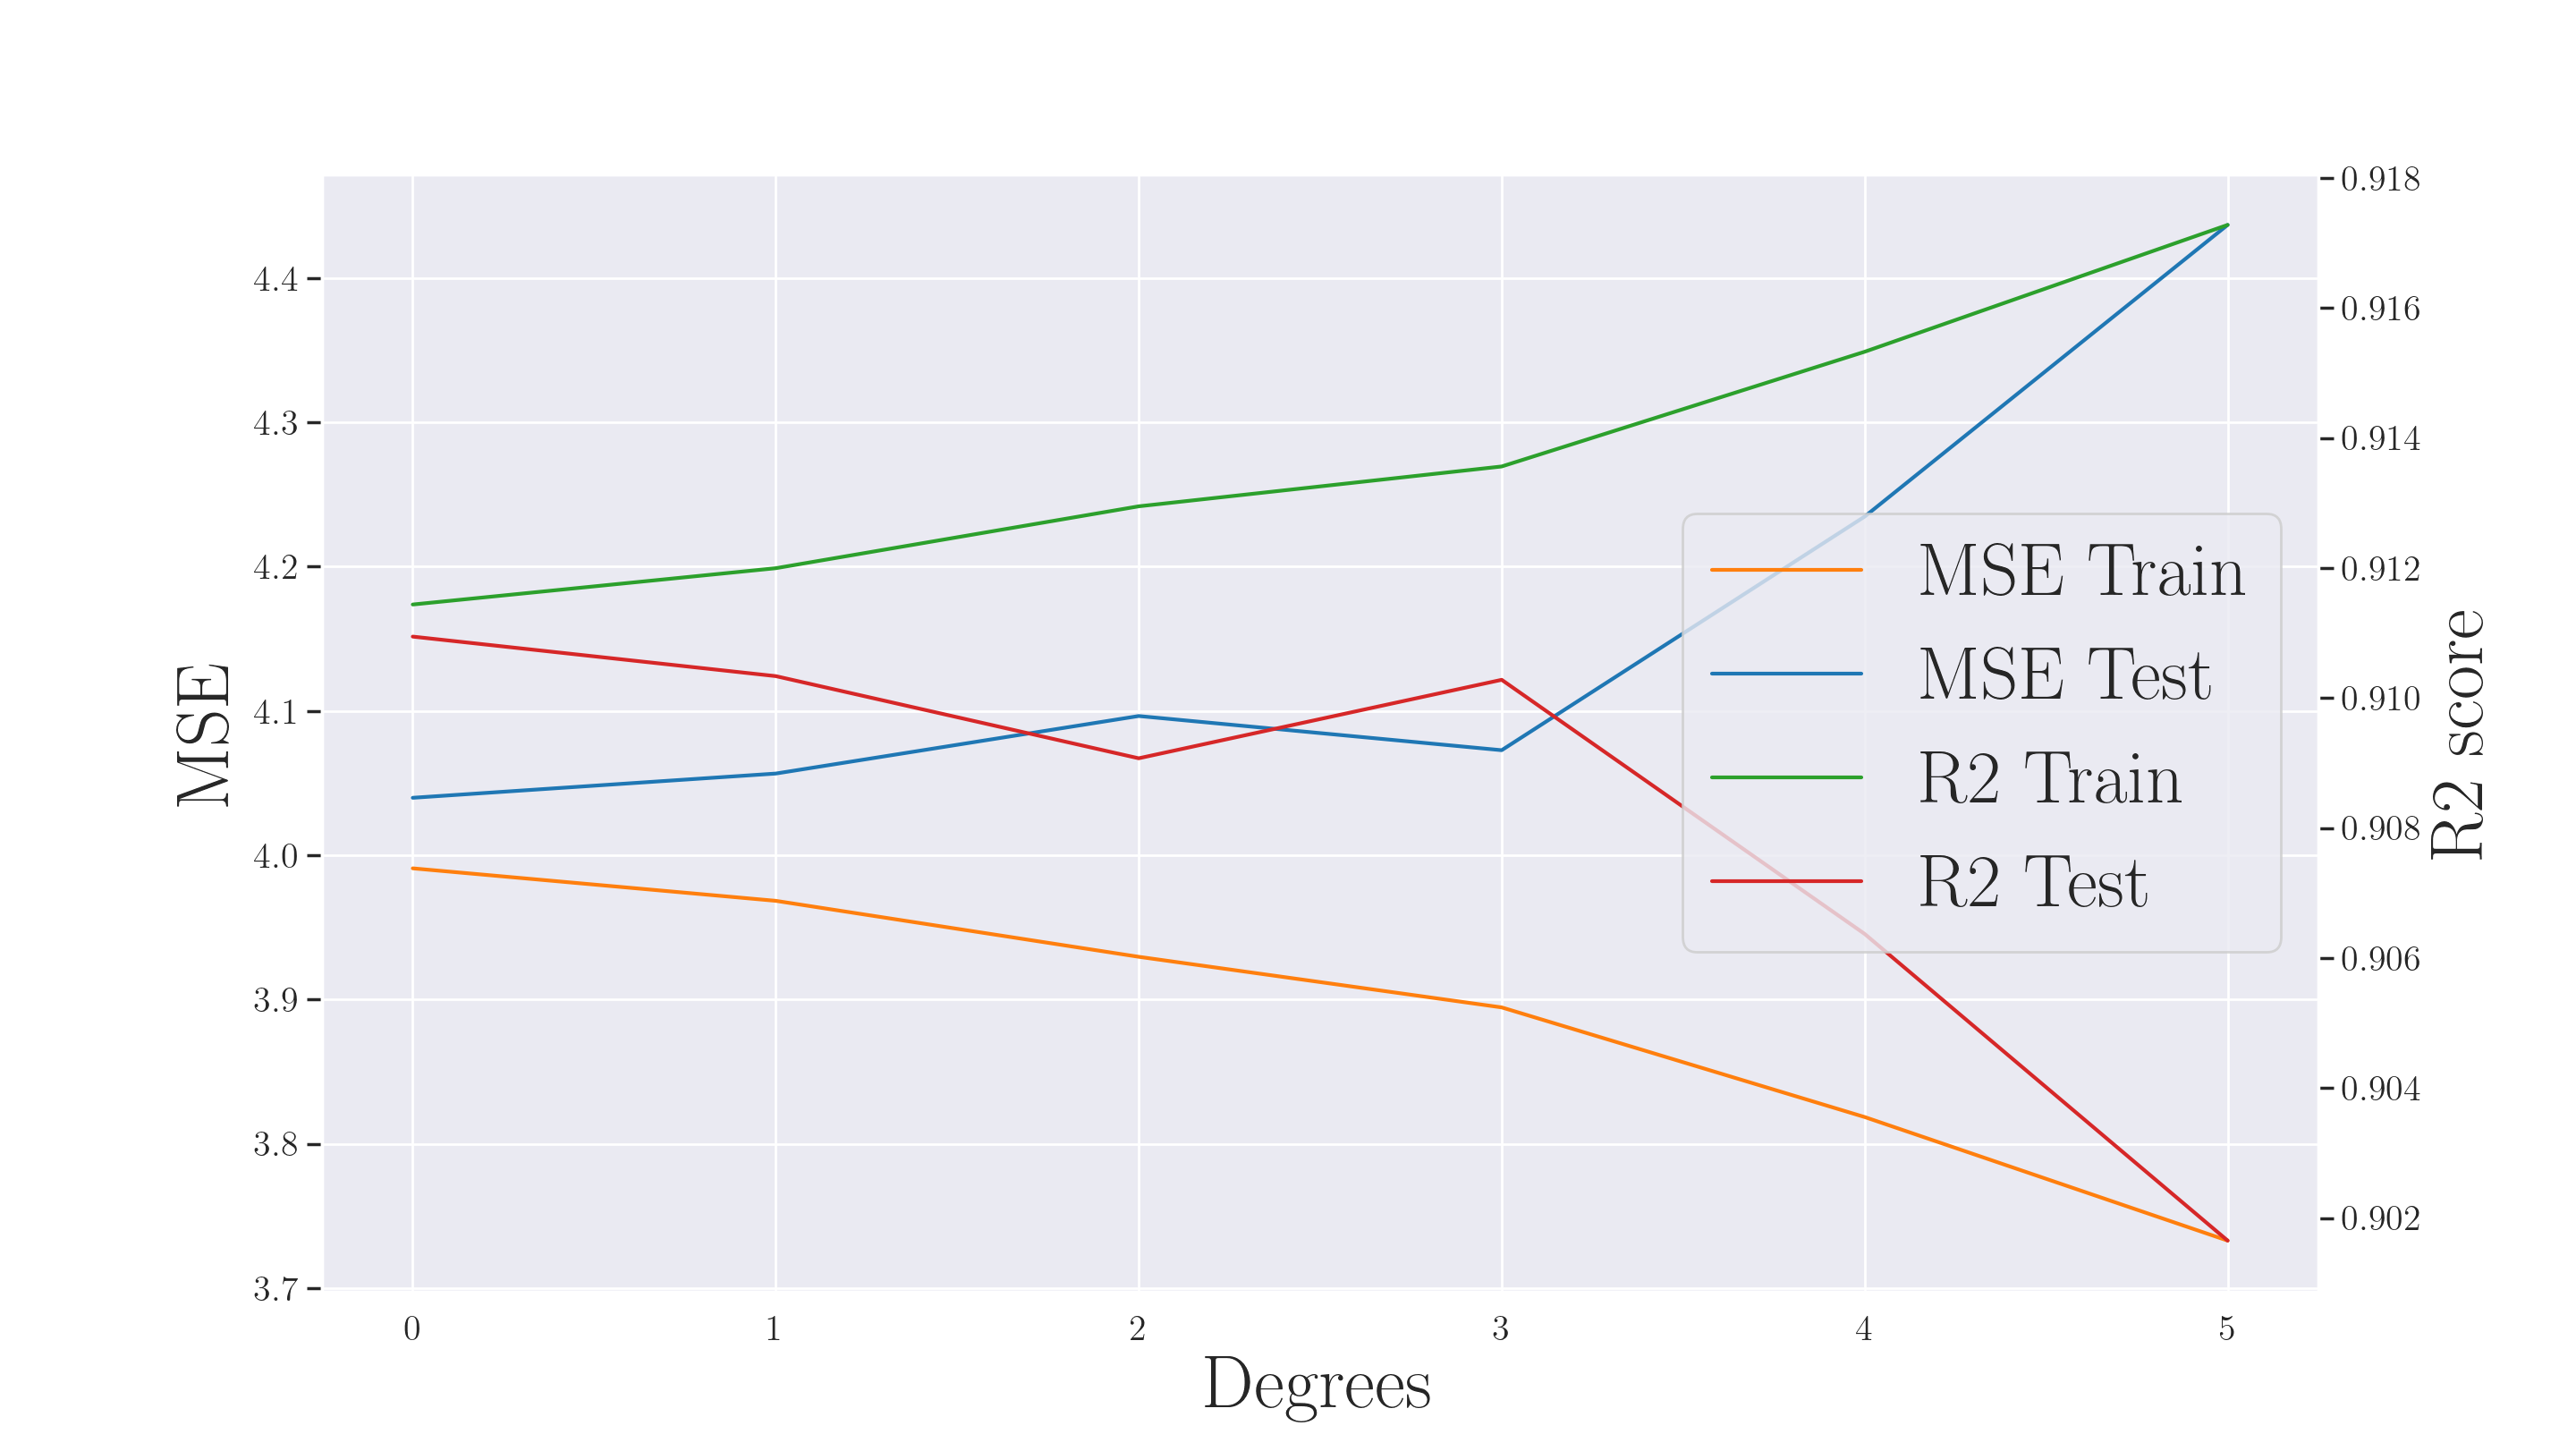
\includegraphics[width=\linewidth]{images/Figure_17.png}
	\caption{A plot of the MSE and R2 score as a function of degrees and a $\lambda$ value of $0$ for Ridge regression on the Franke function with noise given by the normal distribution $\mathcal{N}(0,0.1)$.}
	\label{MSE and R2 Ridge noise lambda0}
\end{figure}
\begin{figure}[H]
	\centering
	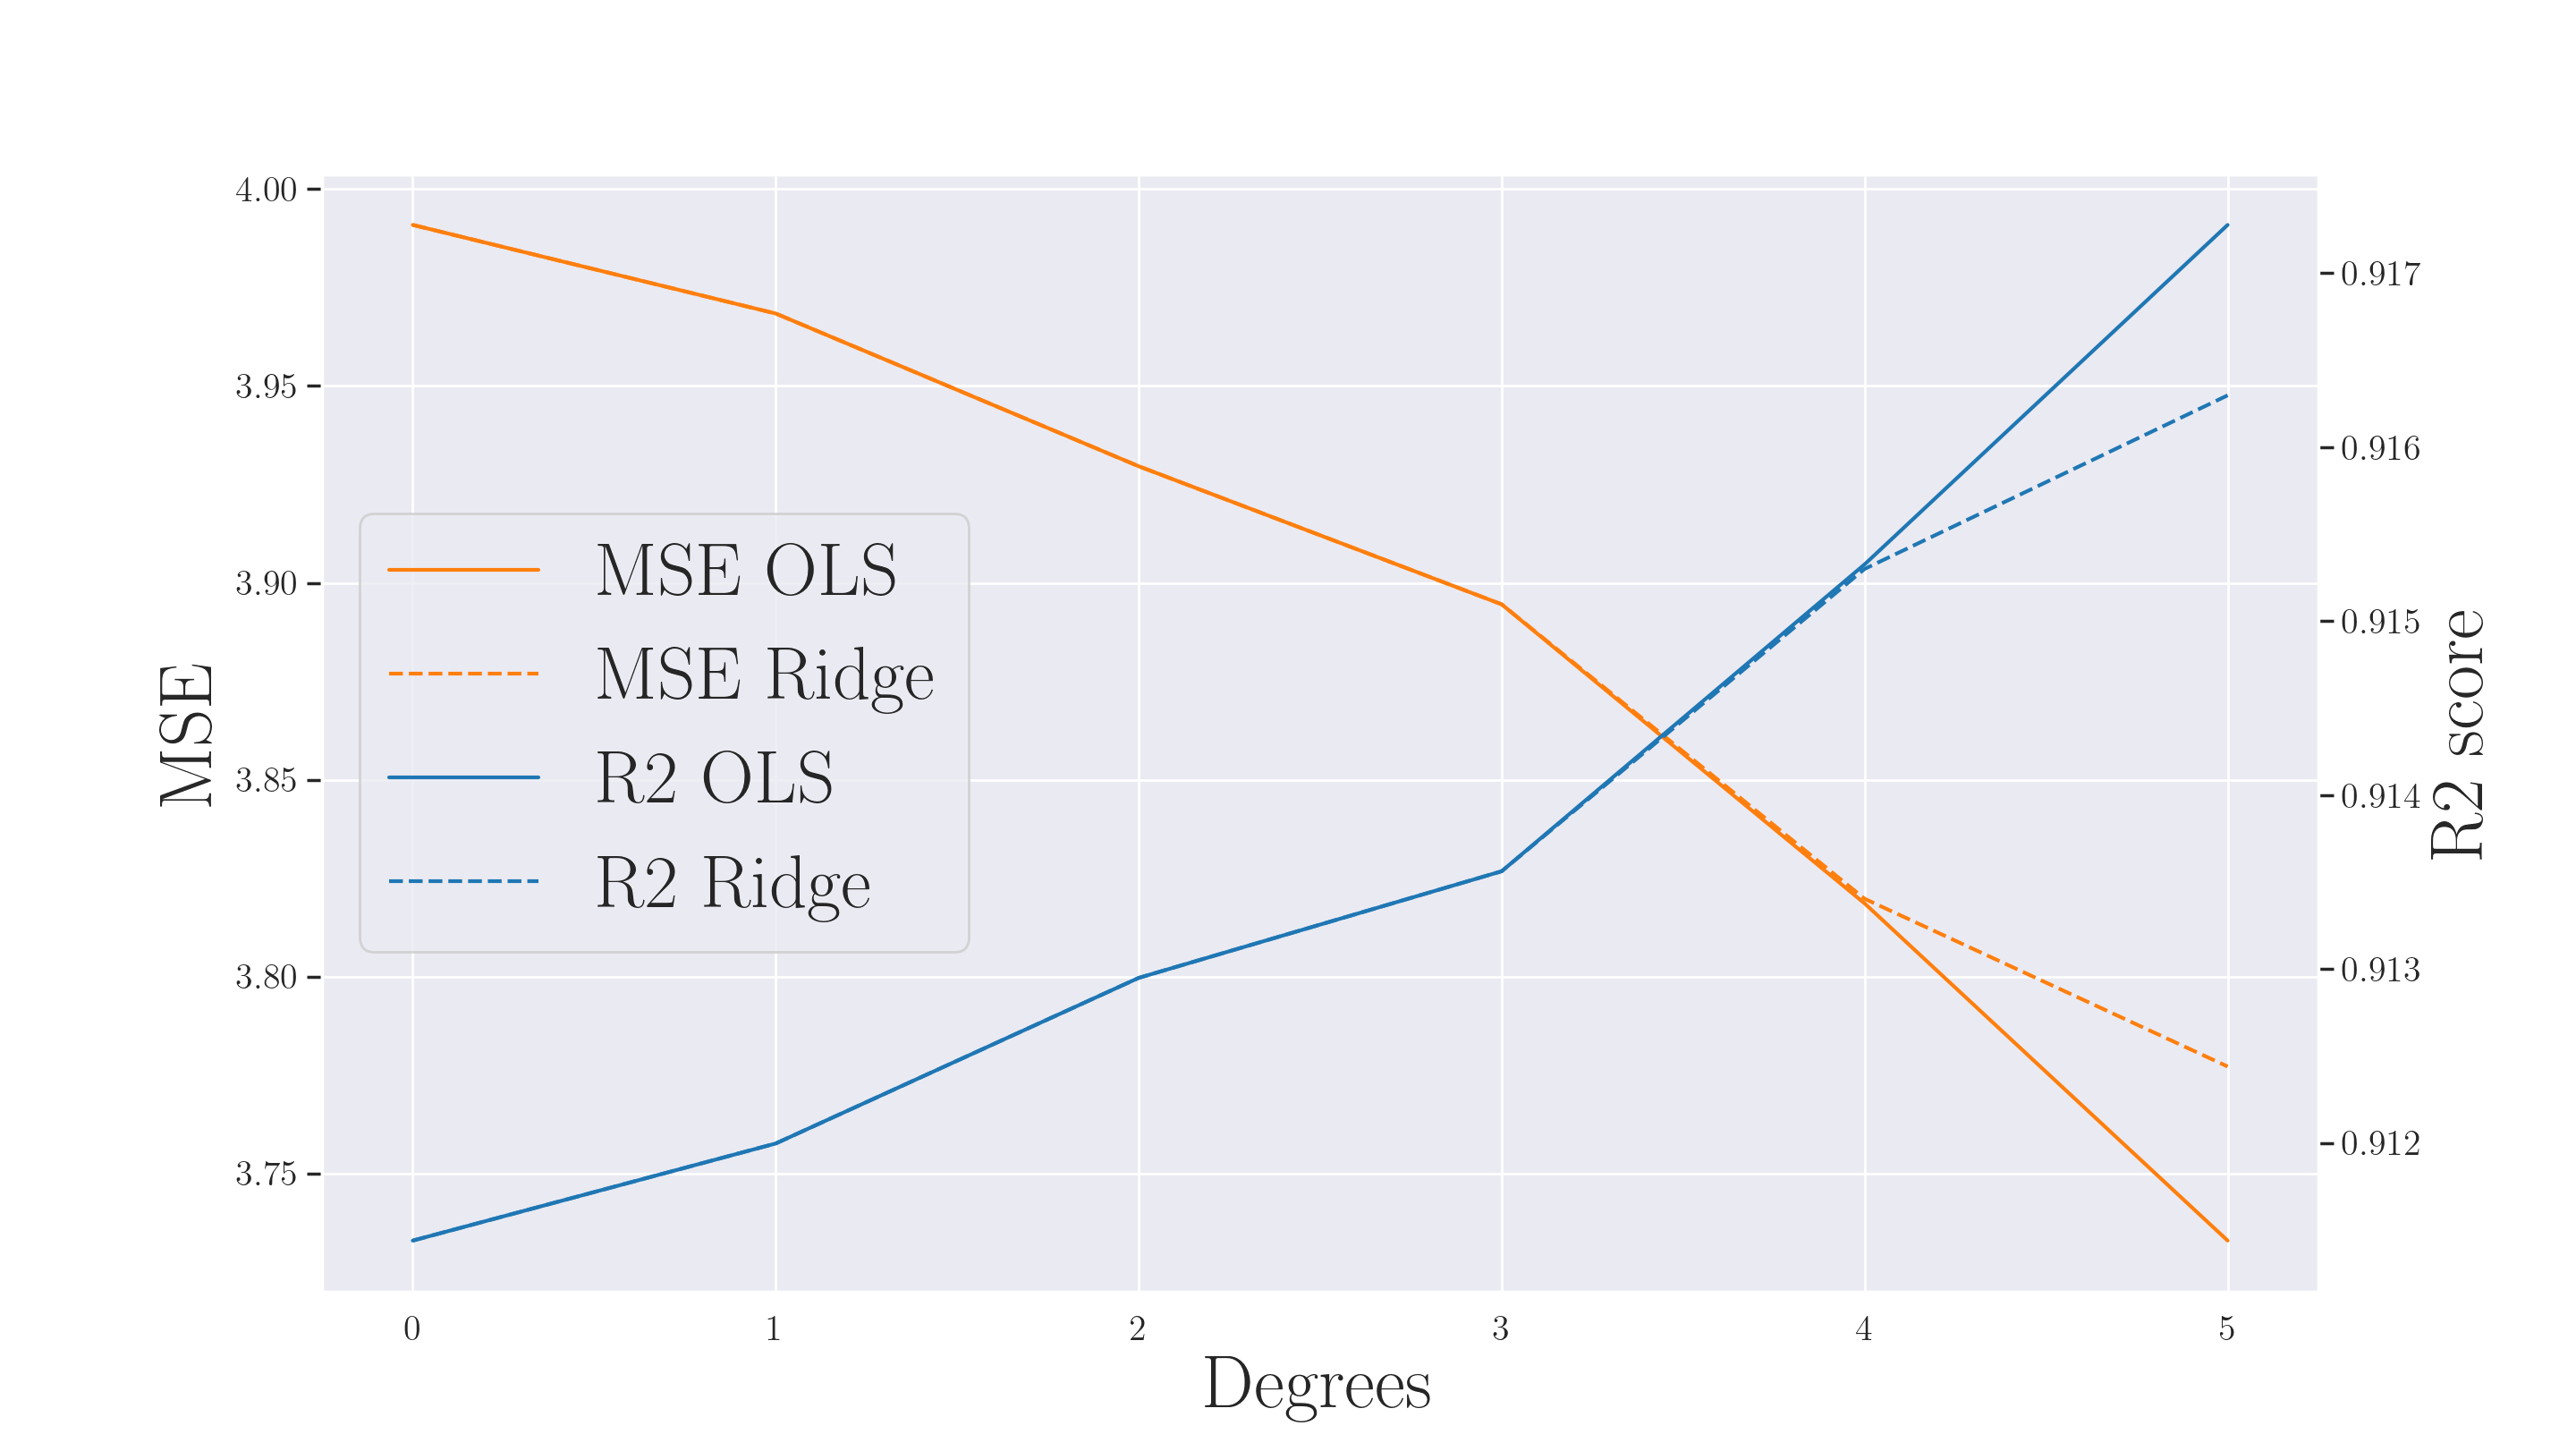
\includegraphics[width=\linewidth]{images/Figure_19.png}
	\caption{A plot of Ridge regression were solid lines shows when $\lambda = 0$, so the same as OLS and the one with doted lines is for $\lambda = 10^{-5}$.}
	\label{Ridge vs OLS}
\end{figure}

\noindent In Figure \eqref{Ridge_crossval_mse_deg} the Mean Squared Error (MSE) is depicted on the $y$-axis, with the logarithm to the base 10 of the hyper parameter $\lambda$ ($\log_{10}(\lambda)$). For the $x$-axis we set the polynomial degrees ranging from 0 - 15. Different lines in varying colors are plotted to showcase the MSE across different $\lambda$ values.
%
\begin{figure}[H]
	\centering
	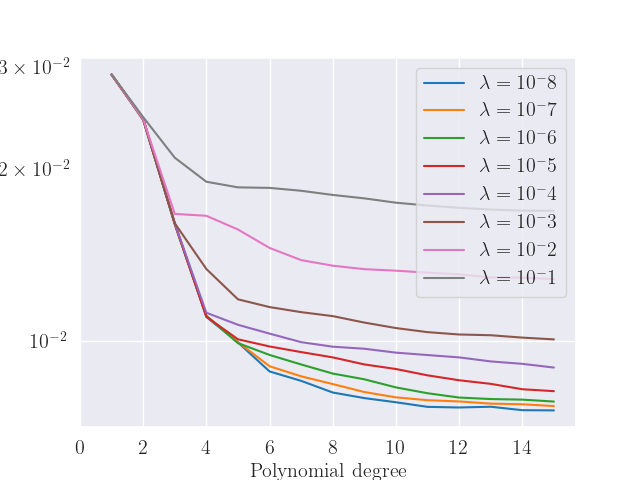
\includegraphics[width=\linewidth]{images/cv_ridge.png}
	\caption{MSE of ridge prediction error for polynomial degree $0-15$, using the Franke function, with cross validation $k=5$.}
 \label{Ridge_crossval_mse_deg}
\end{figure}
%
\noindent Lastly for Ridge regression we plot the $\beta$ values for different complexities in figure \eqref{beta Ridge}. 
\begin{figure}[H]
	\centering
	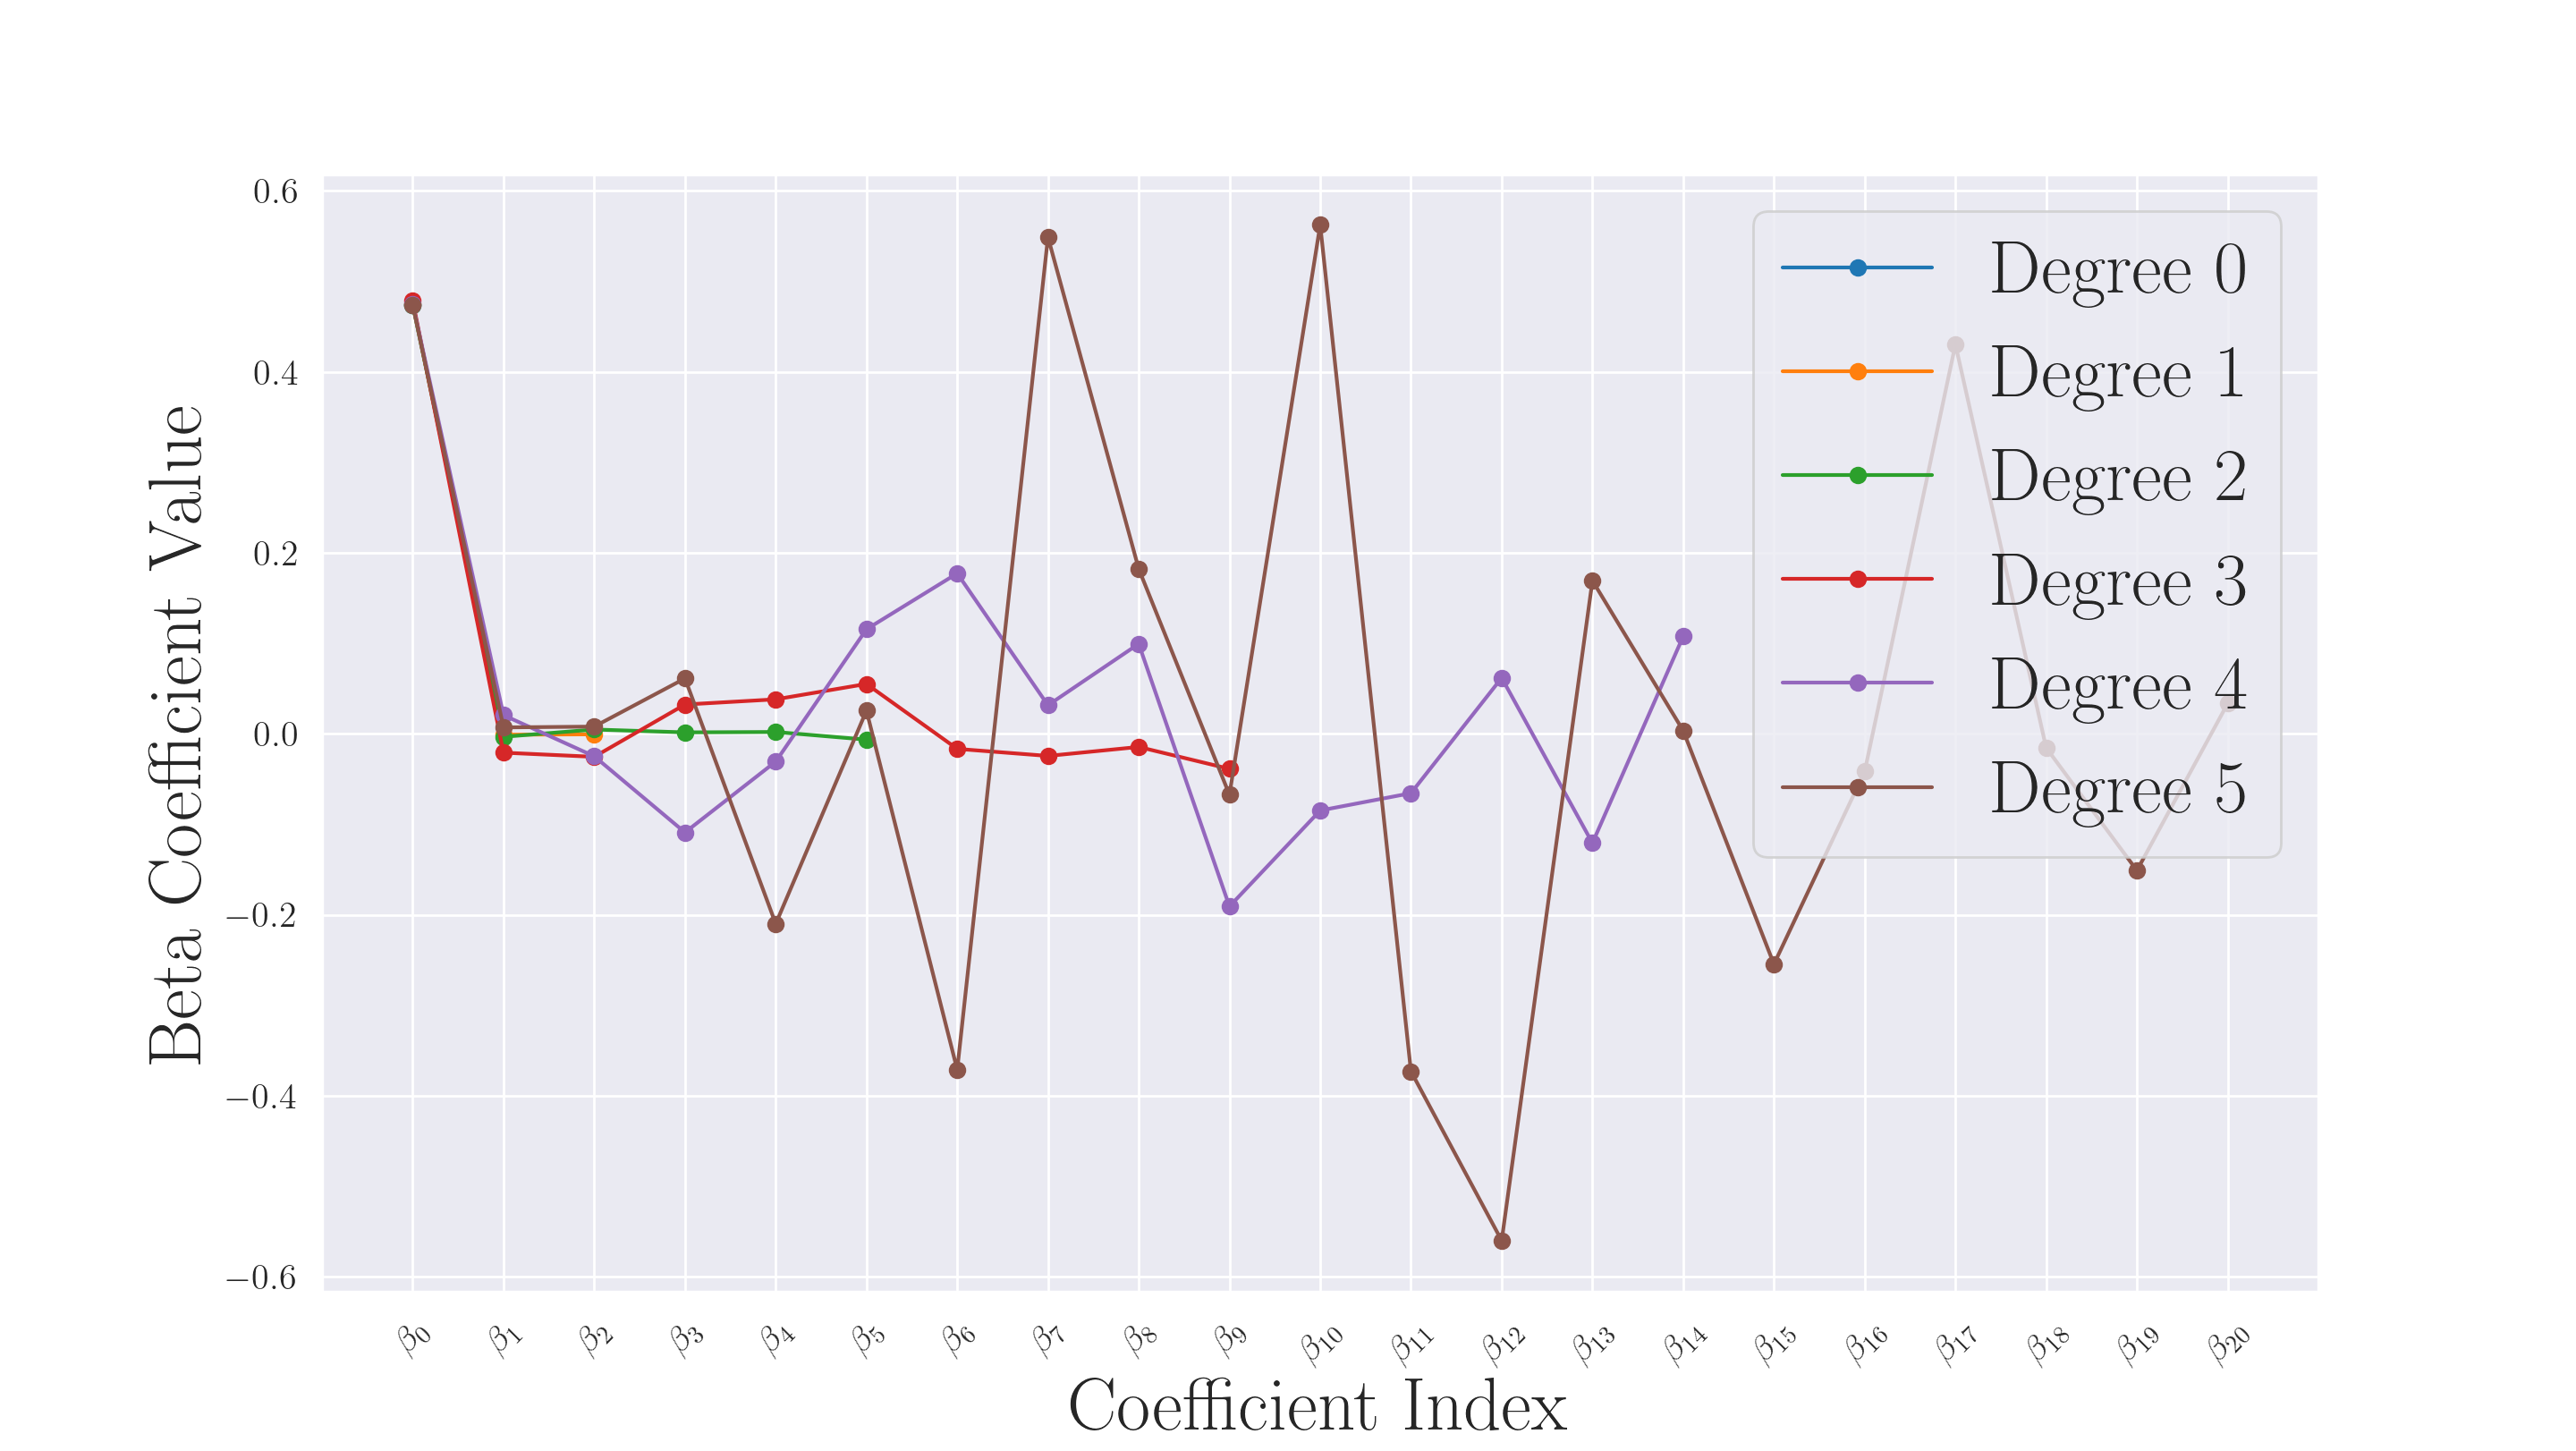
\includegraphics[width=\linewidth]{images/Figure_34.png}
	\caption{A plot showing the $\beta$ values for OLS for different orders of polynomials.}
	\label{beta Ridge}
\end{figure}

\subsubsection{LASSO}
\noindent For LASSO regression we started by making heat maps for both the training data (figure \eqref{heat map training LASSO}) and test data (figure \eqref{heat map test LASSO}) with the same $\lambda$ values ($10^{-8}$ to $10^{2}$) and polynomial degrees (1-5) like for Ridge regression .

\begin{figure}[H]
	\centering
	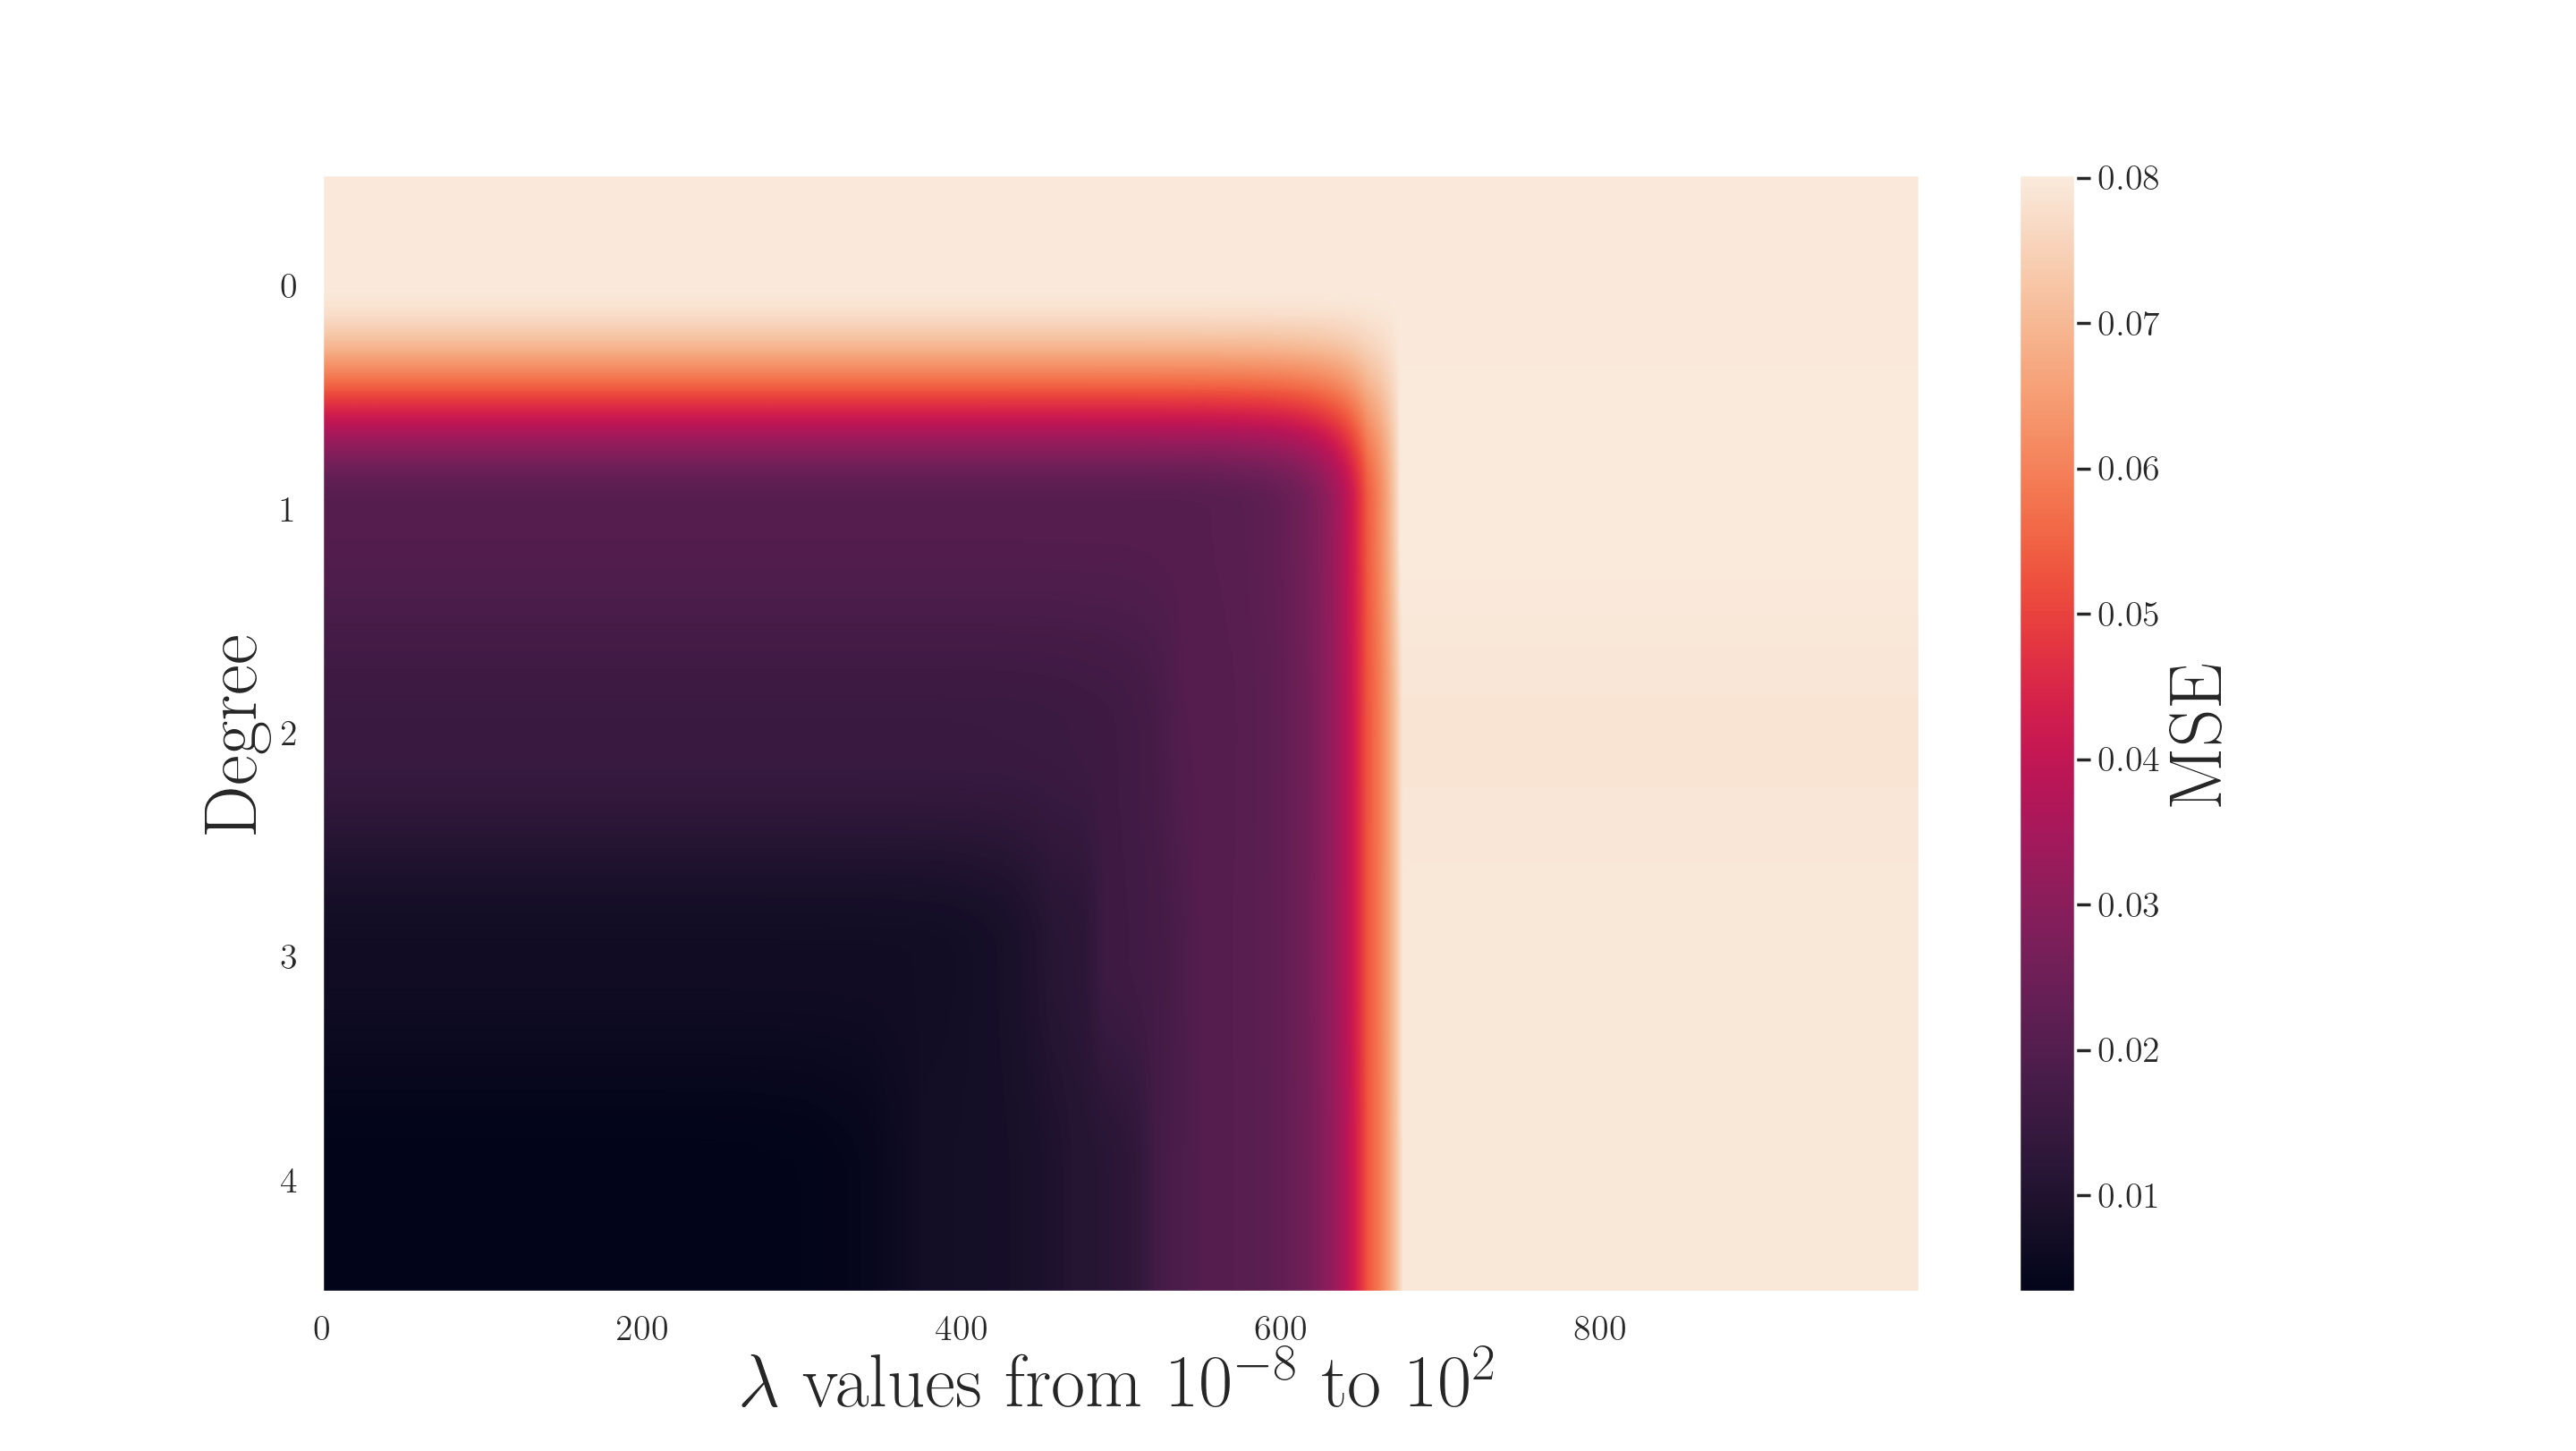
\includegraphics[width=\linewidth]{images/Figure_9.png}
	\caption{A heat map of the MSE for the training data, for different $\lambda$ values and complexities. The $\lambda$ values goes from $10^{-8}$ to $10^{2}$. }
	\label{heat map training LASSO}
\end{figure}
%
\begin{figure}[H]
	\centering
	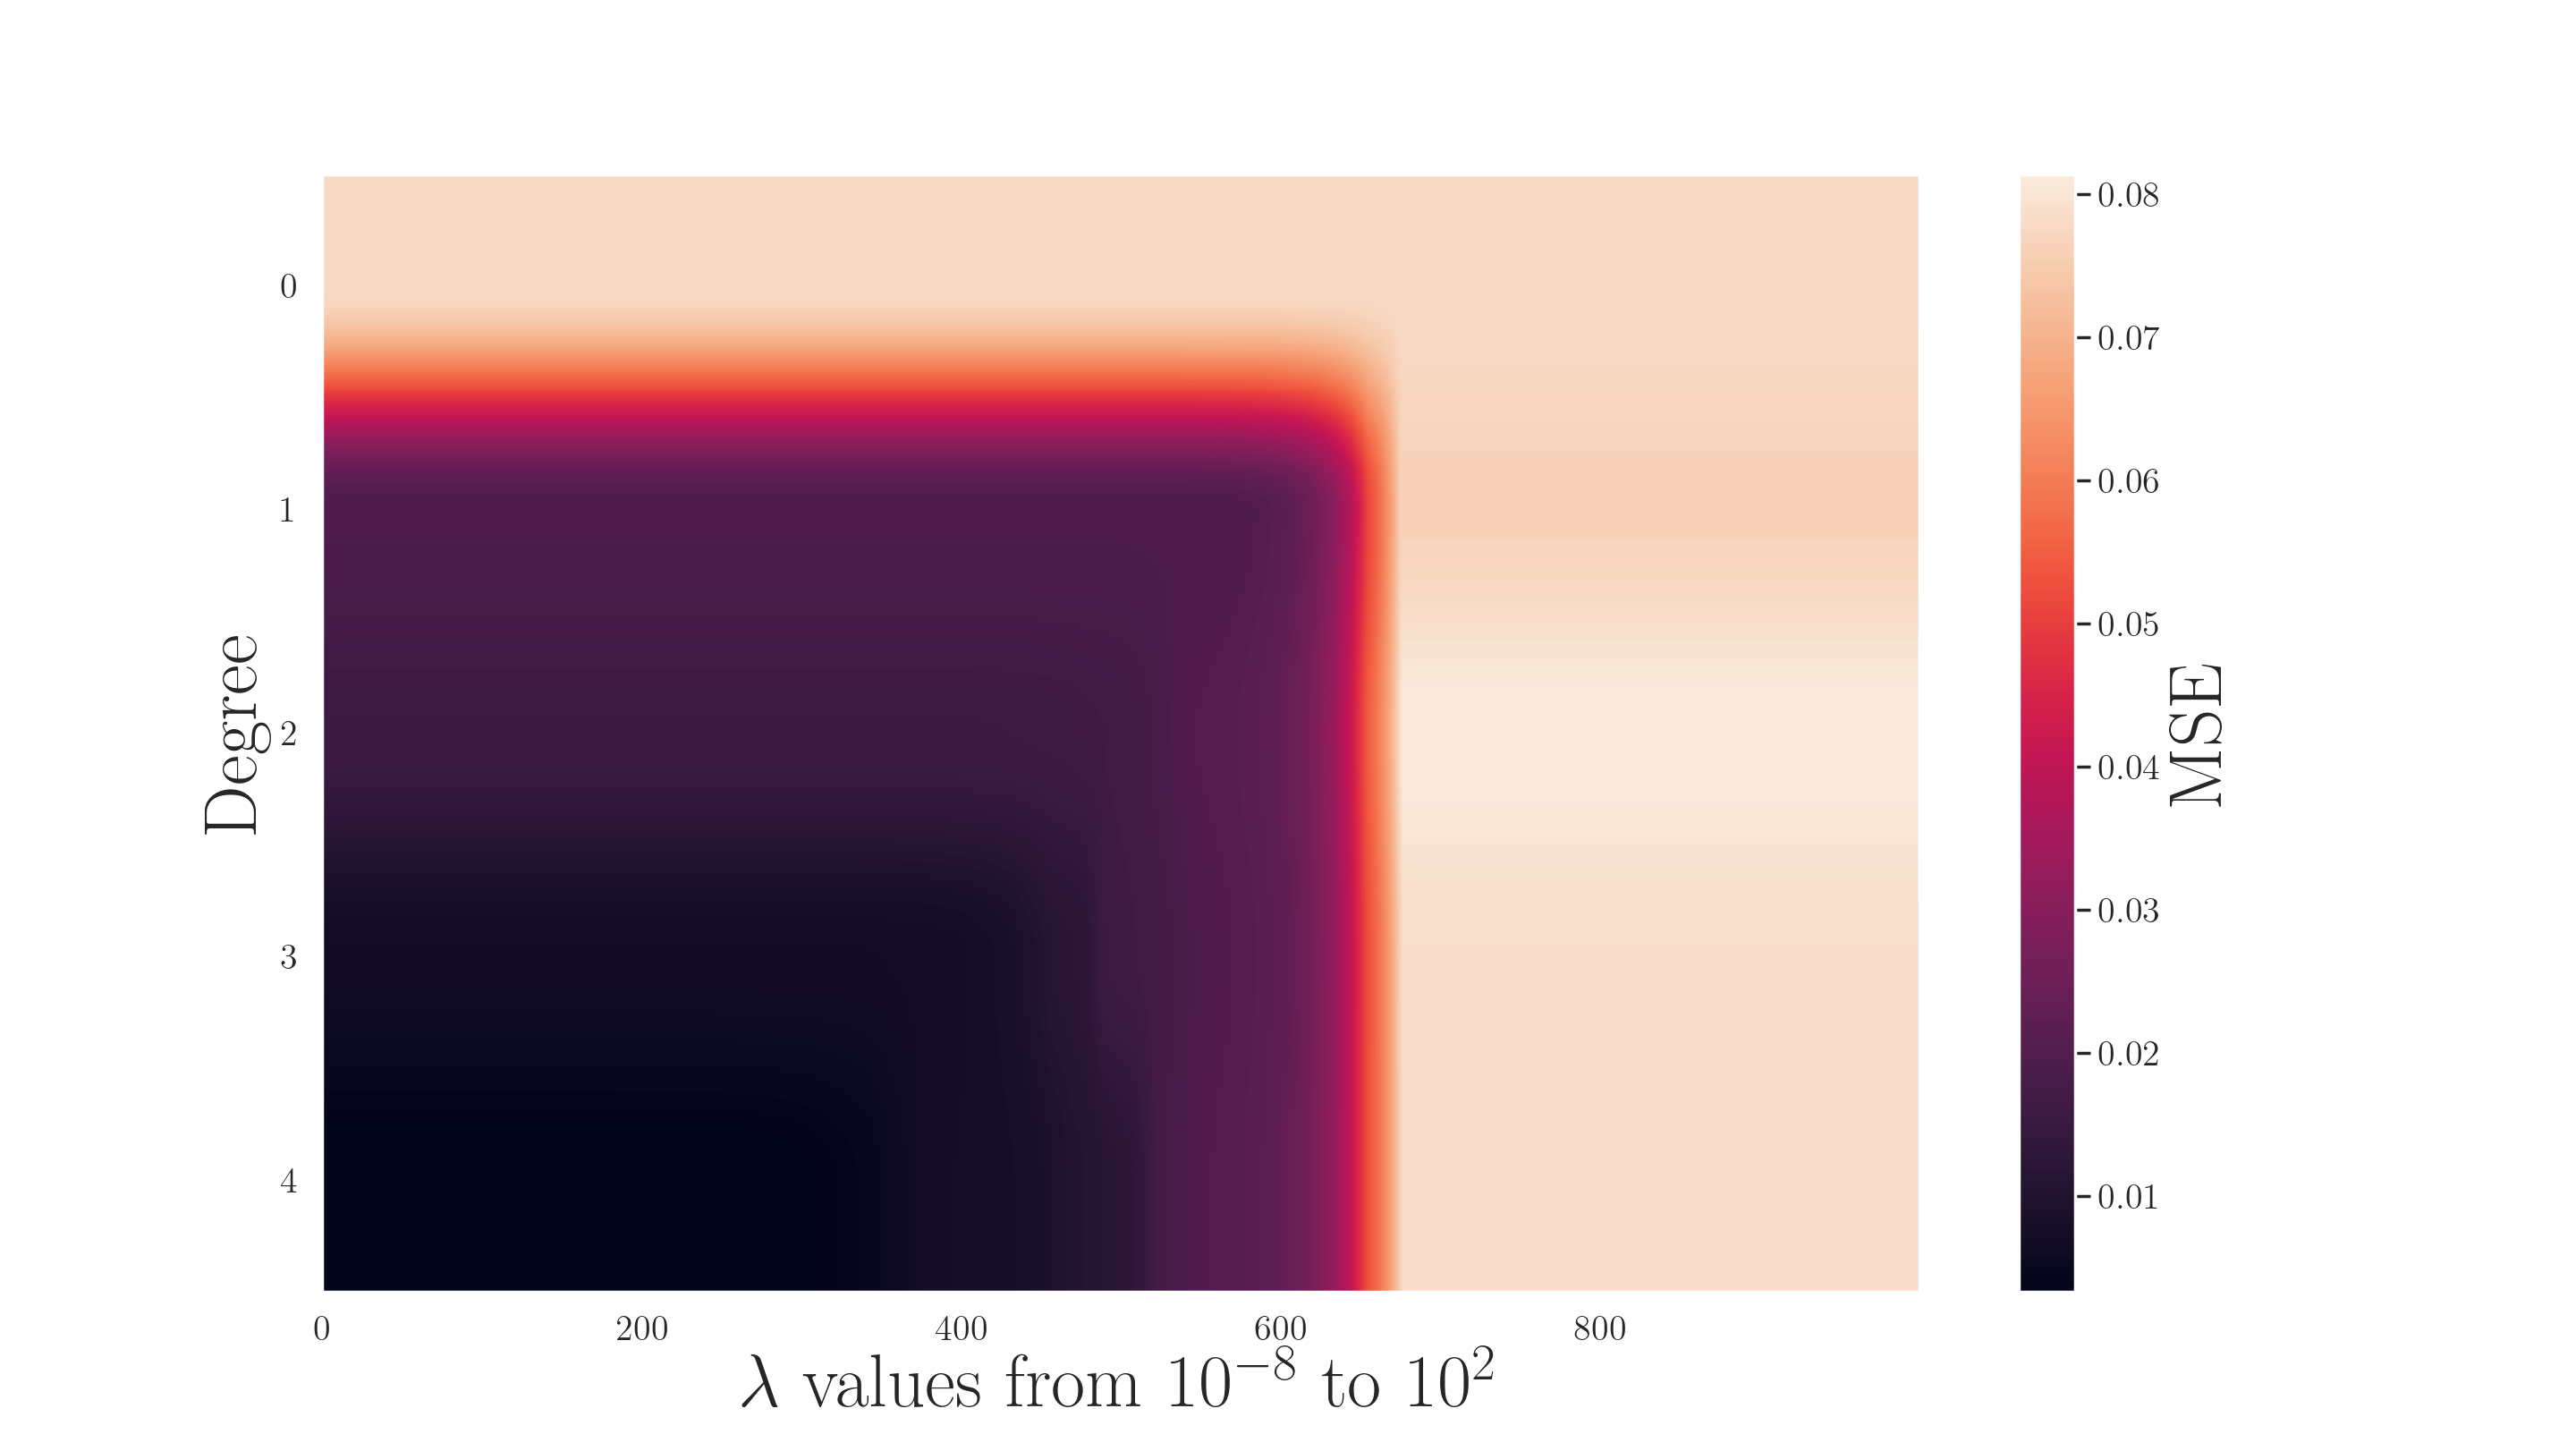
\includegraphics[width=\linewidth]{images/Figure_10.png}
	\caption{A heat map of the MSE for the testing data, for different $\lambda$ values and complexities. The $\lambda$ values goes from $10^{-8}$ to $10^{2}$.}
	\label{heat map test LASSO}
\end{figure}
%
\noindent We then plotted the MSE and R2 score as a function of complexity both without noise (figure \eqref{MSE_and_R2_Lasso_no_noise}) and with noise given by the normal distribution $\mathcal{N}(0,0.1)$ (figure \eqref{MSE_and_R2_Lasso_noise}) for $\lambda = 10^{-5}$.
%
\begin{figure}[H]
    \centering
    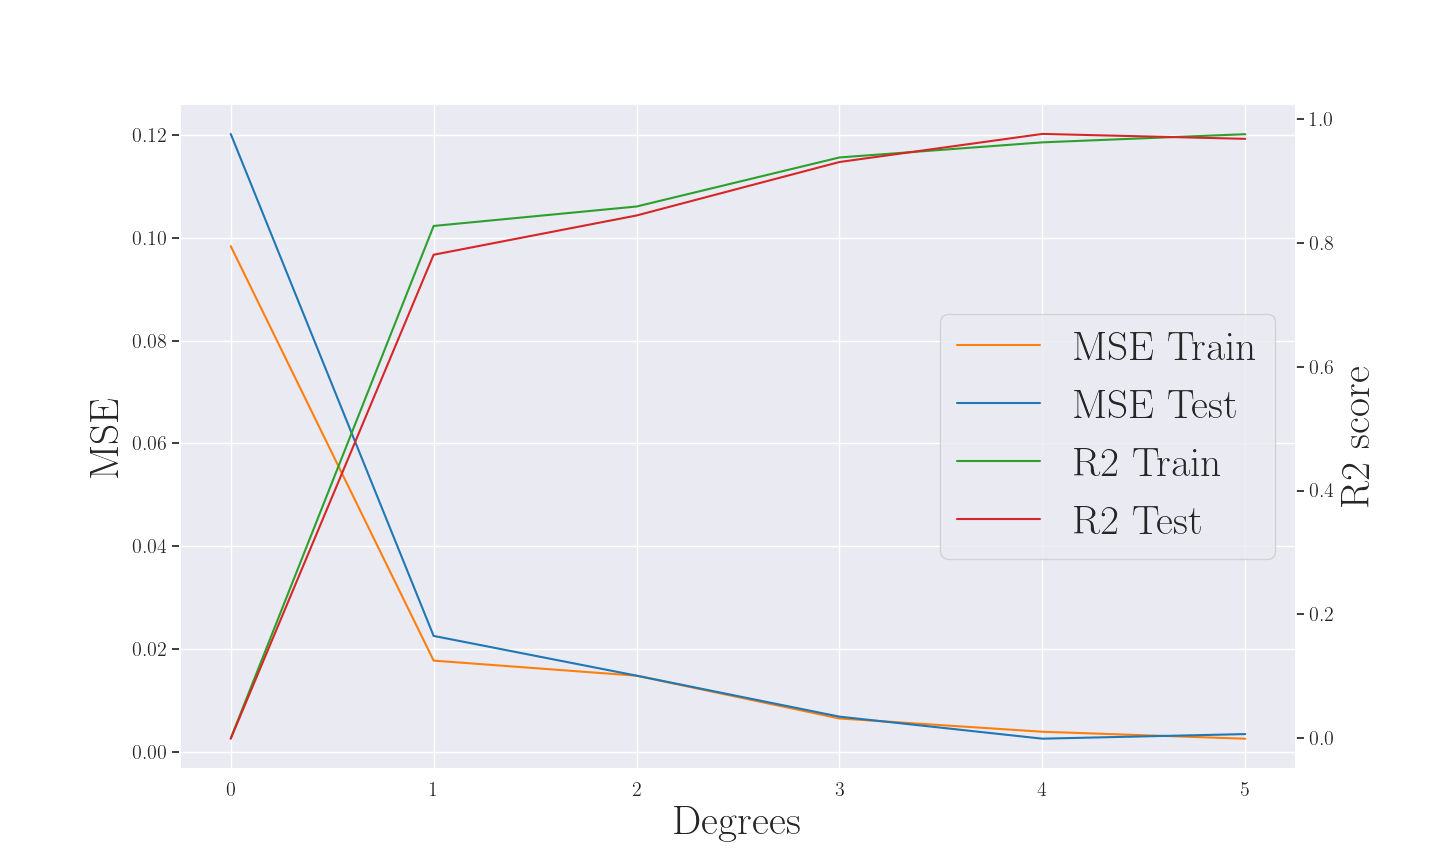
\includegraphics[width=\linewidth]
    {images/MSE_and_R2_Lasso.png}
    \caption{A plot of the MSE and R2 score as a function of degrees and a $\lambda$ value of $10^{-5}$ for LASSO regression on the Franke function with no noise present.} \label{MSE_and_R2_Lasso_no_noise}
\end{figure}
%
\begin{figure}[H]
    \centering
    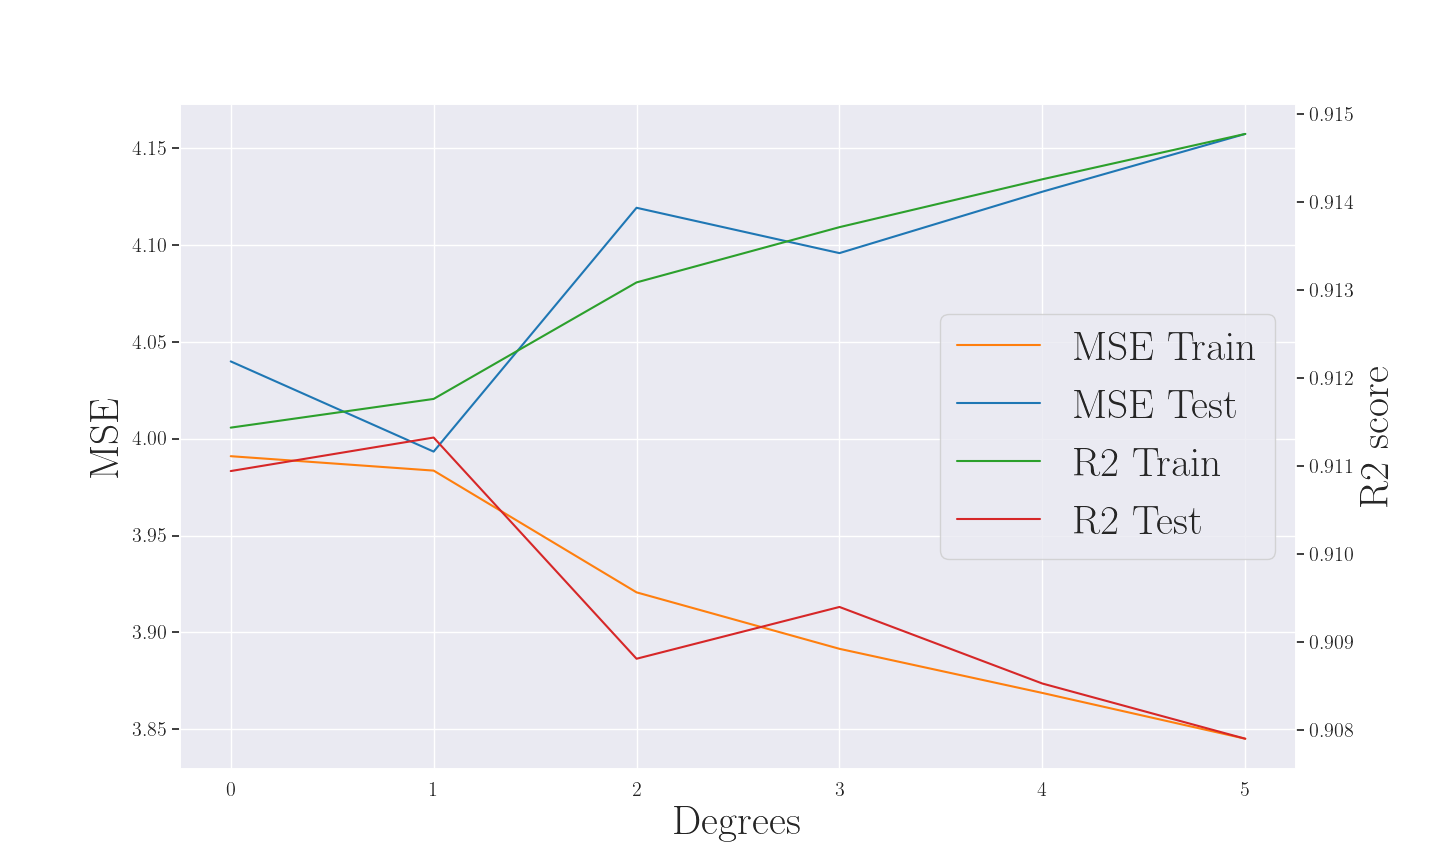
\includegraphics[width=\linewidth]{images/MSE_and_R2_Lasso_noise.png}
    \caption{A plot of the MSE and R2 score as a function of degrees and a $\lambda$ value of $10^{-5}$ for LASSO regression on the Franke function with noise given by the normal distribution $\mathcal{N}(0,0.1)$.} \label{MSE_and_R2_Lasso_noise}
\end{figure}
%
\noindent We then plotted the MSE for OLS, Ridge ($\lambda = 10^{-5}$) and LASSO ($\lambda = 10^{-5}$) given in figure \eqref{OLS_Ridge_and_Lasso} . 
%
\begin{figure}[H]
	\centering
	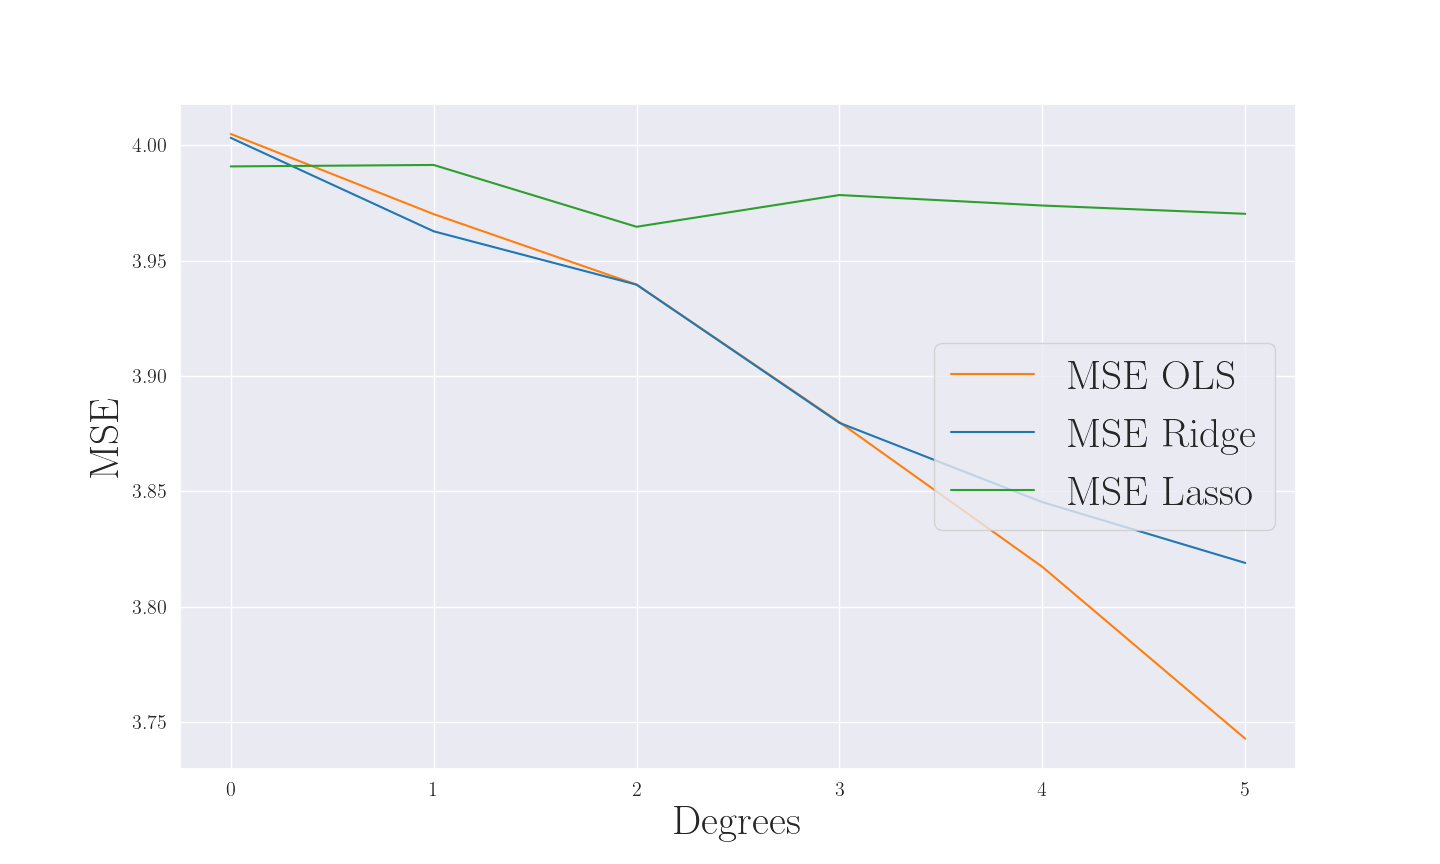
\includegraphics[width=\linewidth]{images/MSE_for_OLS_Ridge_Lasso.png}
	\caption{A plot of OLS, Ridge regression with $\lambda = 10^{-5}$ and LASSO regression with $\lambda = 10^{-5}$ on the Franke function with noise given by the normal distribution $\mathcal{N}(0,0.1)$. }
	\label{OLS_Ridge_and_Lasso}
\end{figure}
%
\noindent In Figure \eqref{Lasso_crossval_mse_deg}, the Mean Squared Error (MSE) is plotted on the $y$-axis in a logarithmic scale. The $x$-axis represents the polynomial degrees, which range from 0 to 14. Multiple colored lines are shown, each representing a specific value of the regularization parameter $\lambda$. These lines provide a visual representation of the MSE across different $\lambda$ values for varying polynomial degrees, assisting in the determination of an optimal polynomial degree and regularization parameter for LASSO regression.
%
\begin{figure}[H]
	\centering
	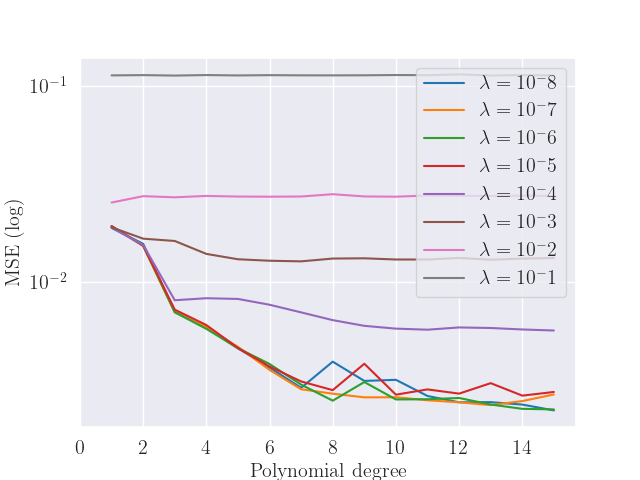
\includegraphics[width=\linewidth]{images/cv_lasso.png}
	\caption{MSE of LASSO prediction error for polynomial degree $0-15$, using the Franke function, with cross validation $k=5$.}
 \label{Lasso_crossval_mse_deg}
\end{figure}

\subsection{Real terrain data}
\subsubsection{OLS}
\noindent Now we look at the analysis of the real terrain data. First we performed a OLS regression on the data set, where we varied the complexity between 0 and 10 degrees. The MSE and R2 score is shown in figure \eqref{OLS terrain data}. 
\begin{figure}[H]
	\centering
	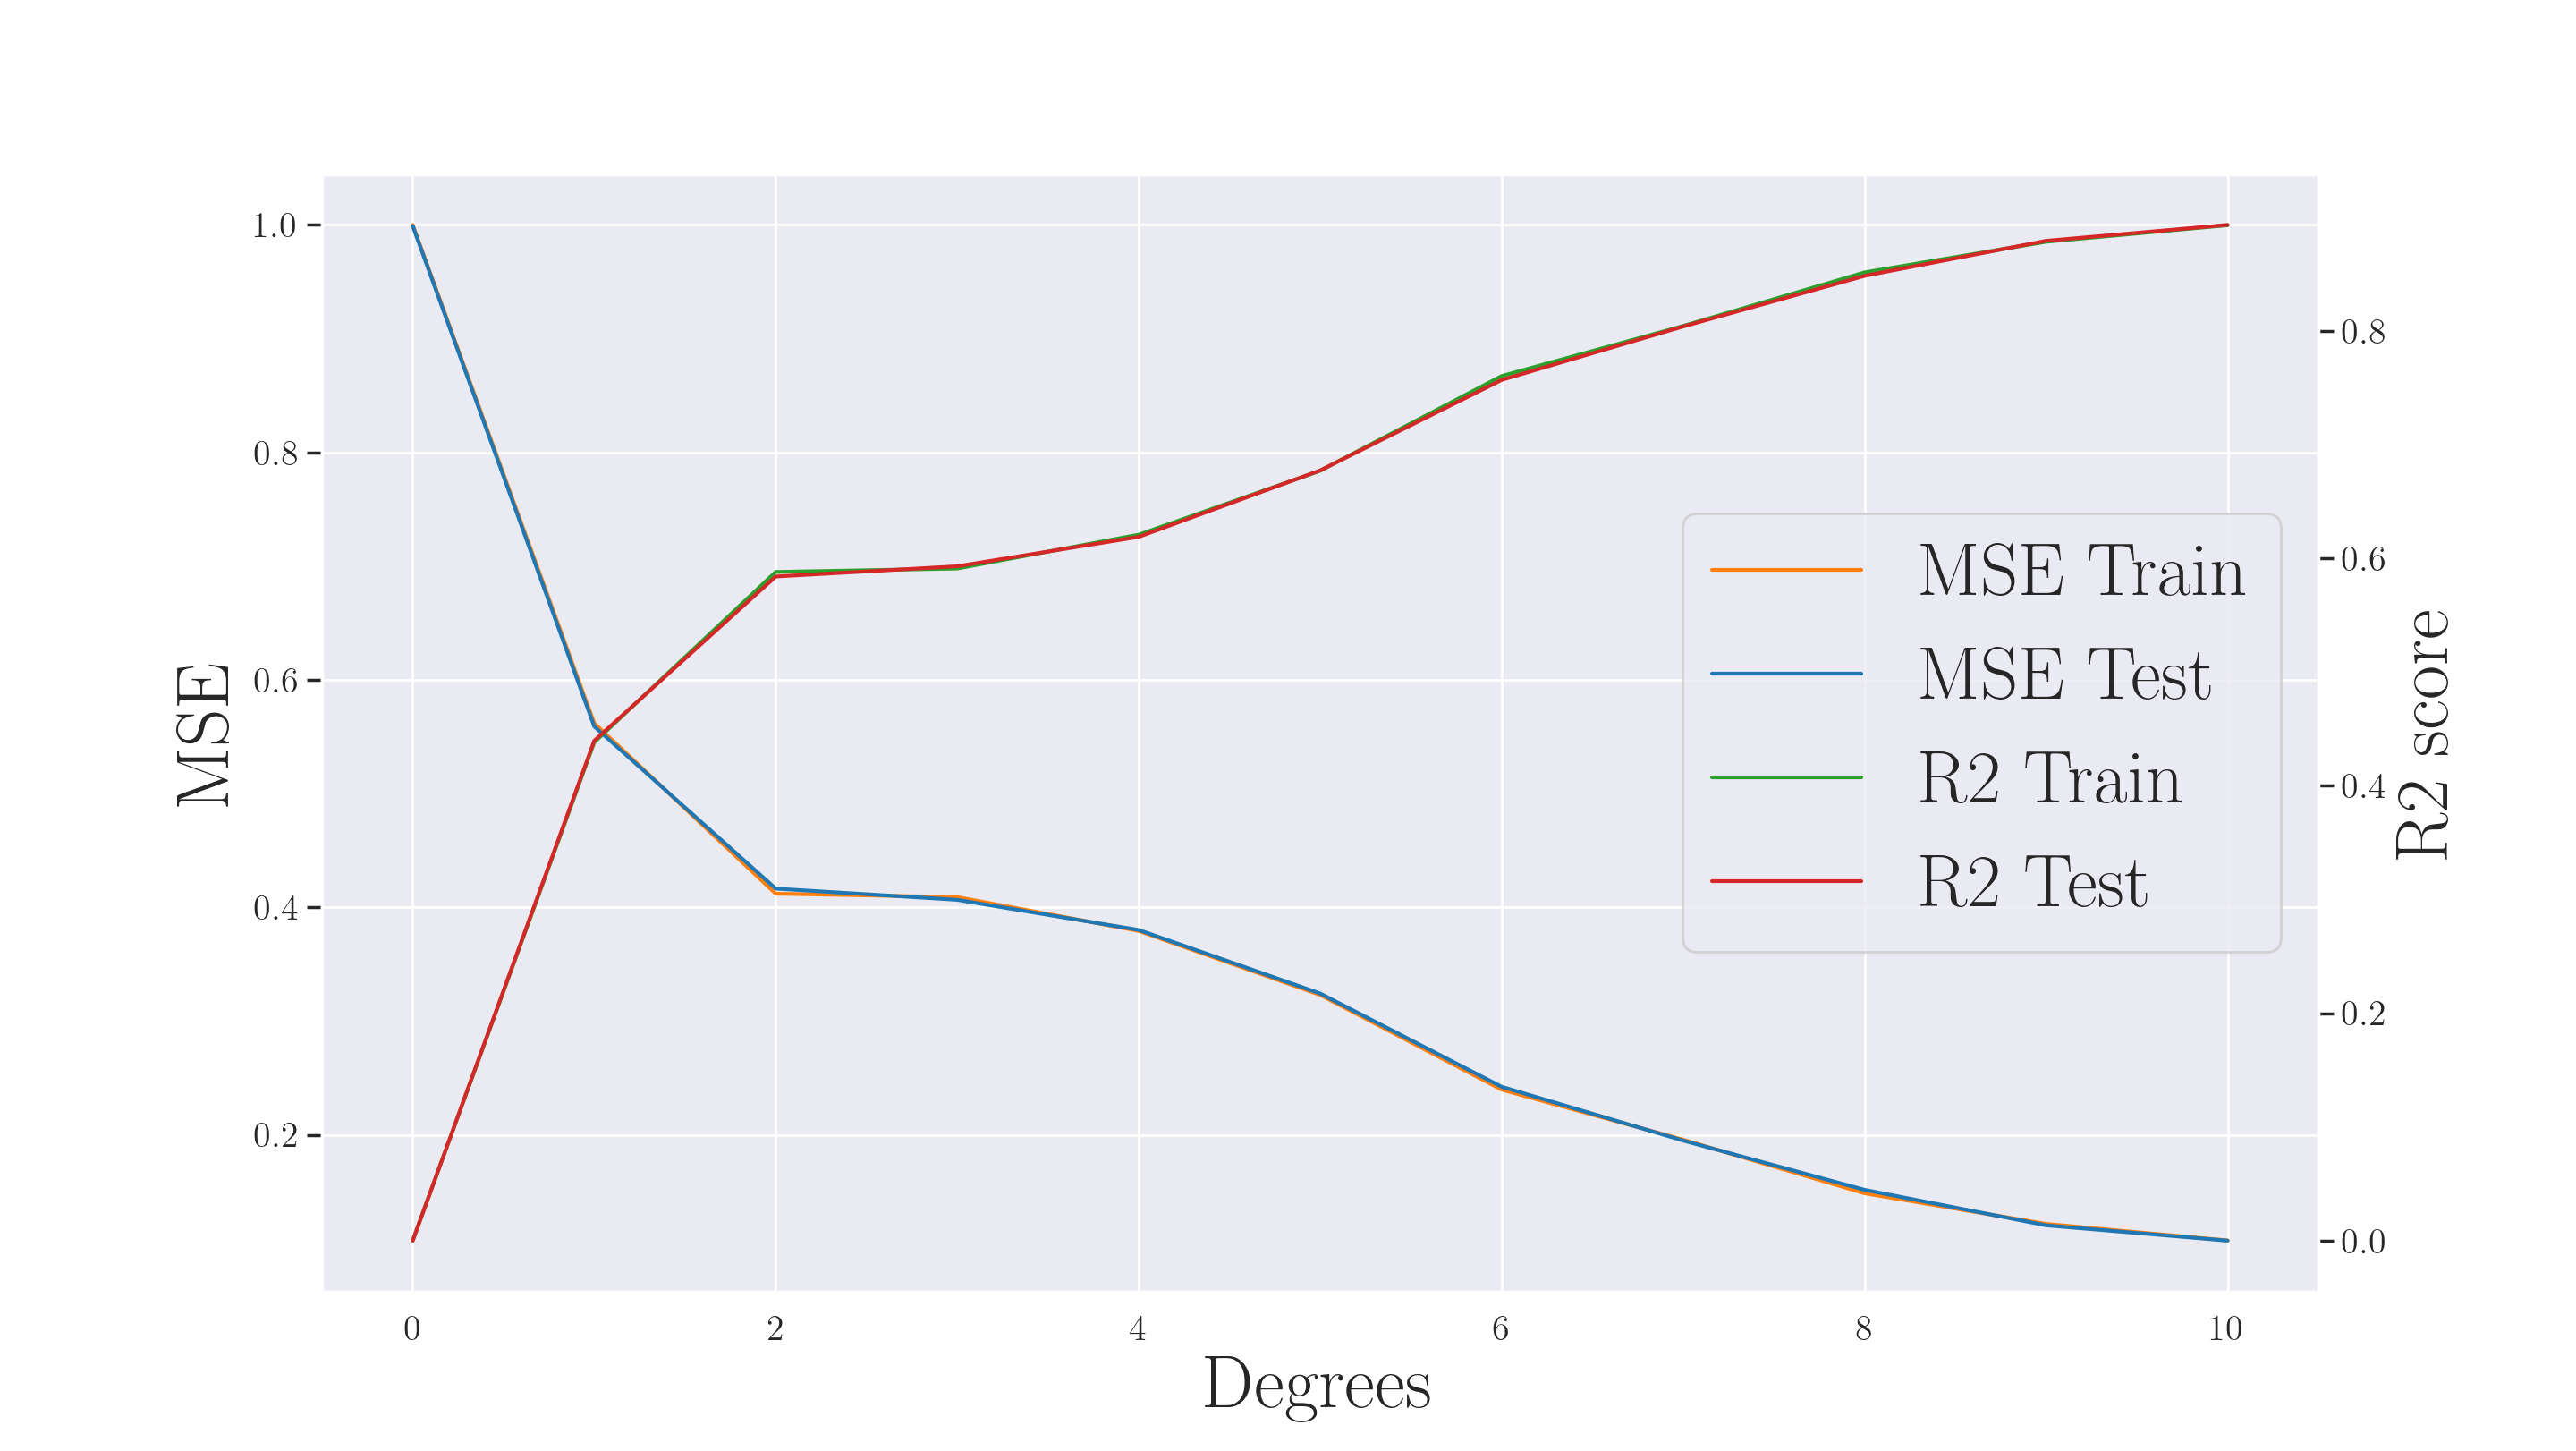
\includegraphics[width=\linewidth]{images/Figure_21.png}
	\caption{A plot showing the MSE and R2 score for the OLS regression on the terrain data.}
	\label{OLS terrain data}
\end{figure}
% Do not think this figura is necerrary since we are comparing Bootstrap and CV in the next figure
% \begin{figure}[H]
%     \centering
%     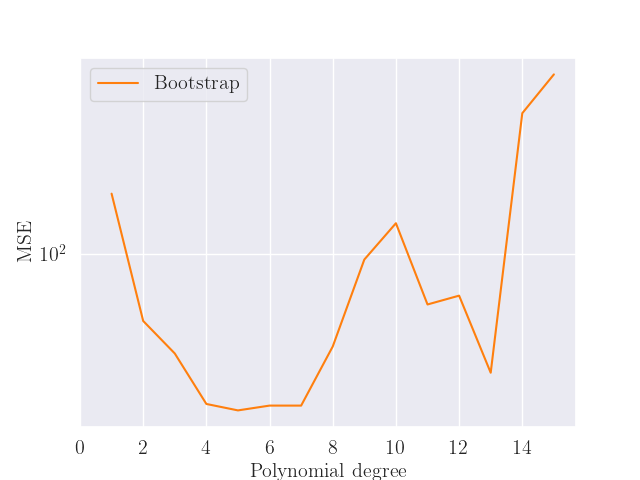
\includegraphics[width=\linewidth]{images/bootstrap_terrain.png}
%     \caption{MSE as a function of complexity for OLS with terrain data, using bootstrap with 100 samples.}
%     \label{fig:bootstrap_terrain}
% \end{figure}
\noindent We compared re-sampling techniques for the terrain data, using OLS as regression method. MSE for both are shown in figure \ref{fig:bootstrap_cv_terrain}. 
\begin{figure}[H]
    \centering
    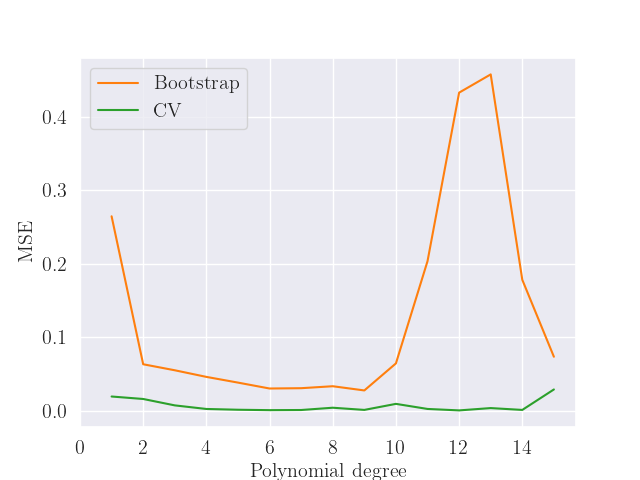
\includegraphics[width=\linewidth]{images/bootstrap_cv_terrain.png}
    \caption{MSE as a function of complexity for OLS with terrain data, using both bootstrap with 100 samples, and cross validation with $k=5$.}
    \label{fig:bootstrap_cv_terrain}
\end{figure}

\subsubsection{Ridge}
\noindent Next we implemented Ridge regression on the terrain data. We made a heat map of the MSE values as a function of $\lambda$ values and complexity. The complexity varied from 1 to 10 and the $\lambda$ values varied from $10^{-8}$ to $10^{2}$. The result is shown in figure \eqref{heat map Ridge Terrain data} and \eqref{heat map Ridge Terrain data test}.
\begin{figure}[H]
	\centering
	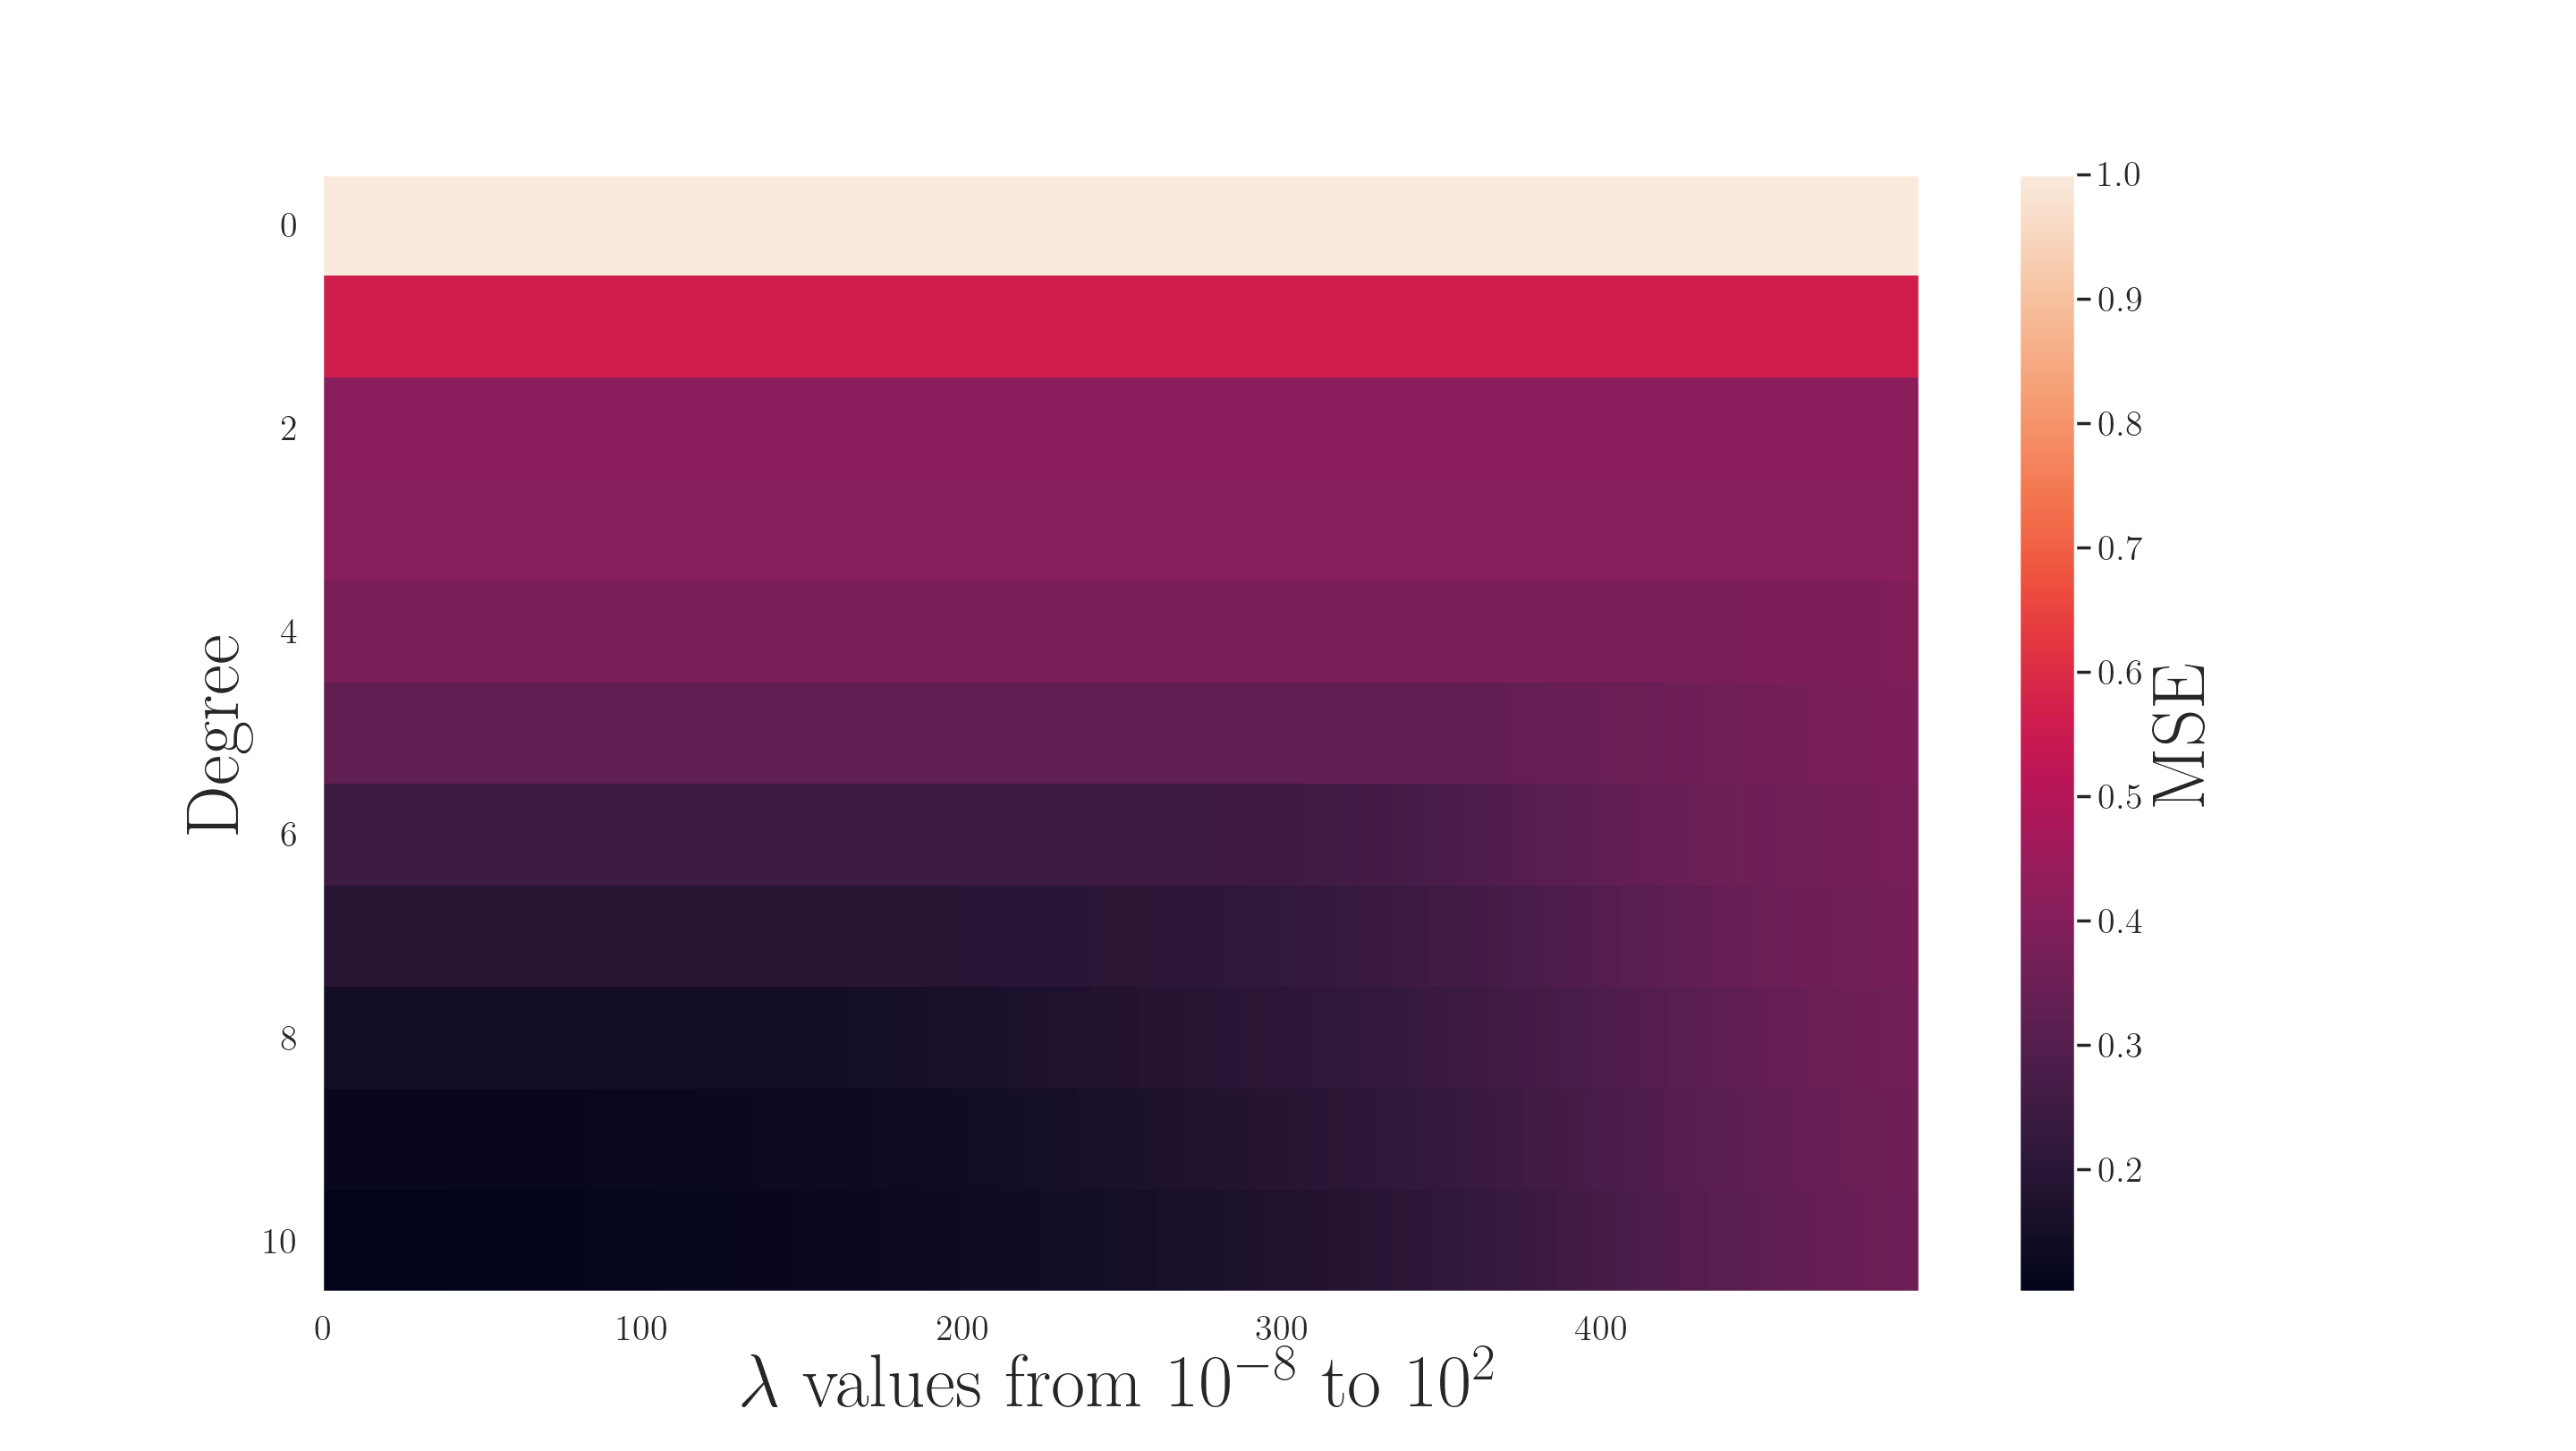
\includegraphics[width=\linewidth]{images/Figure_22.png}
	\caption{Heat map of the MSE for the training data, as a function of complexity and $lambda$ values.}
	\label{heat map Ridge Terrain data}
\end{figure}
%
\begin{figure}[H]
	\centering
	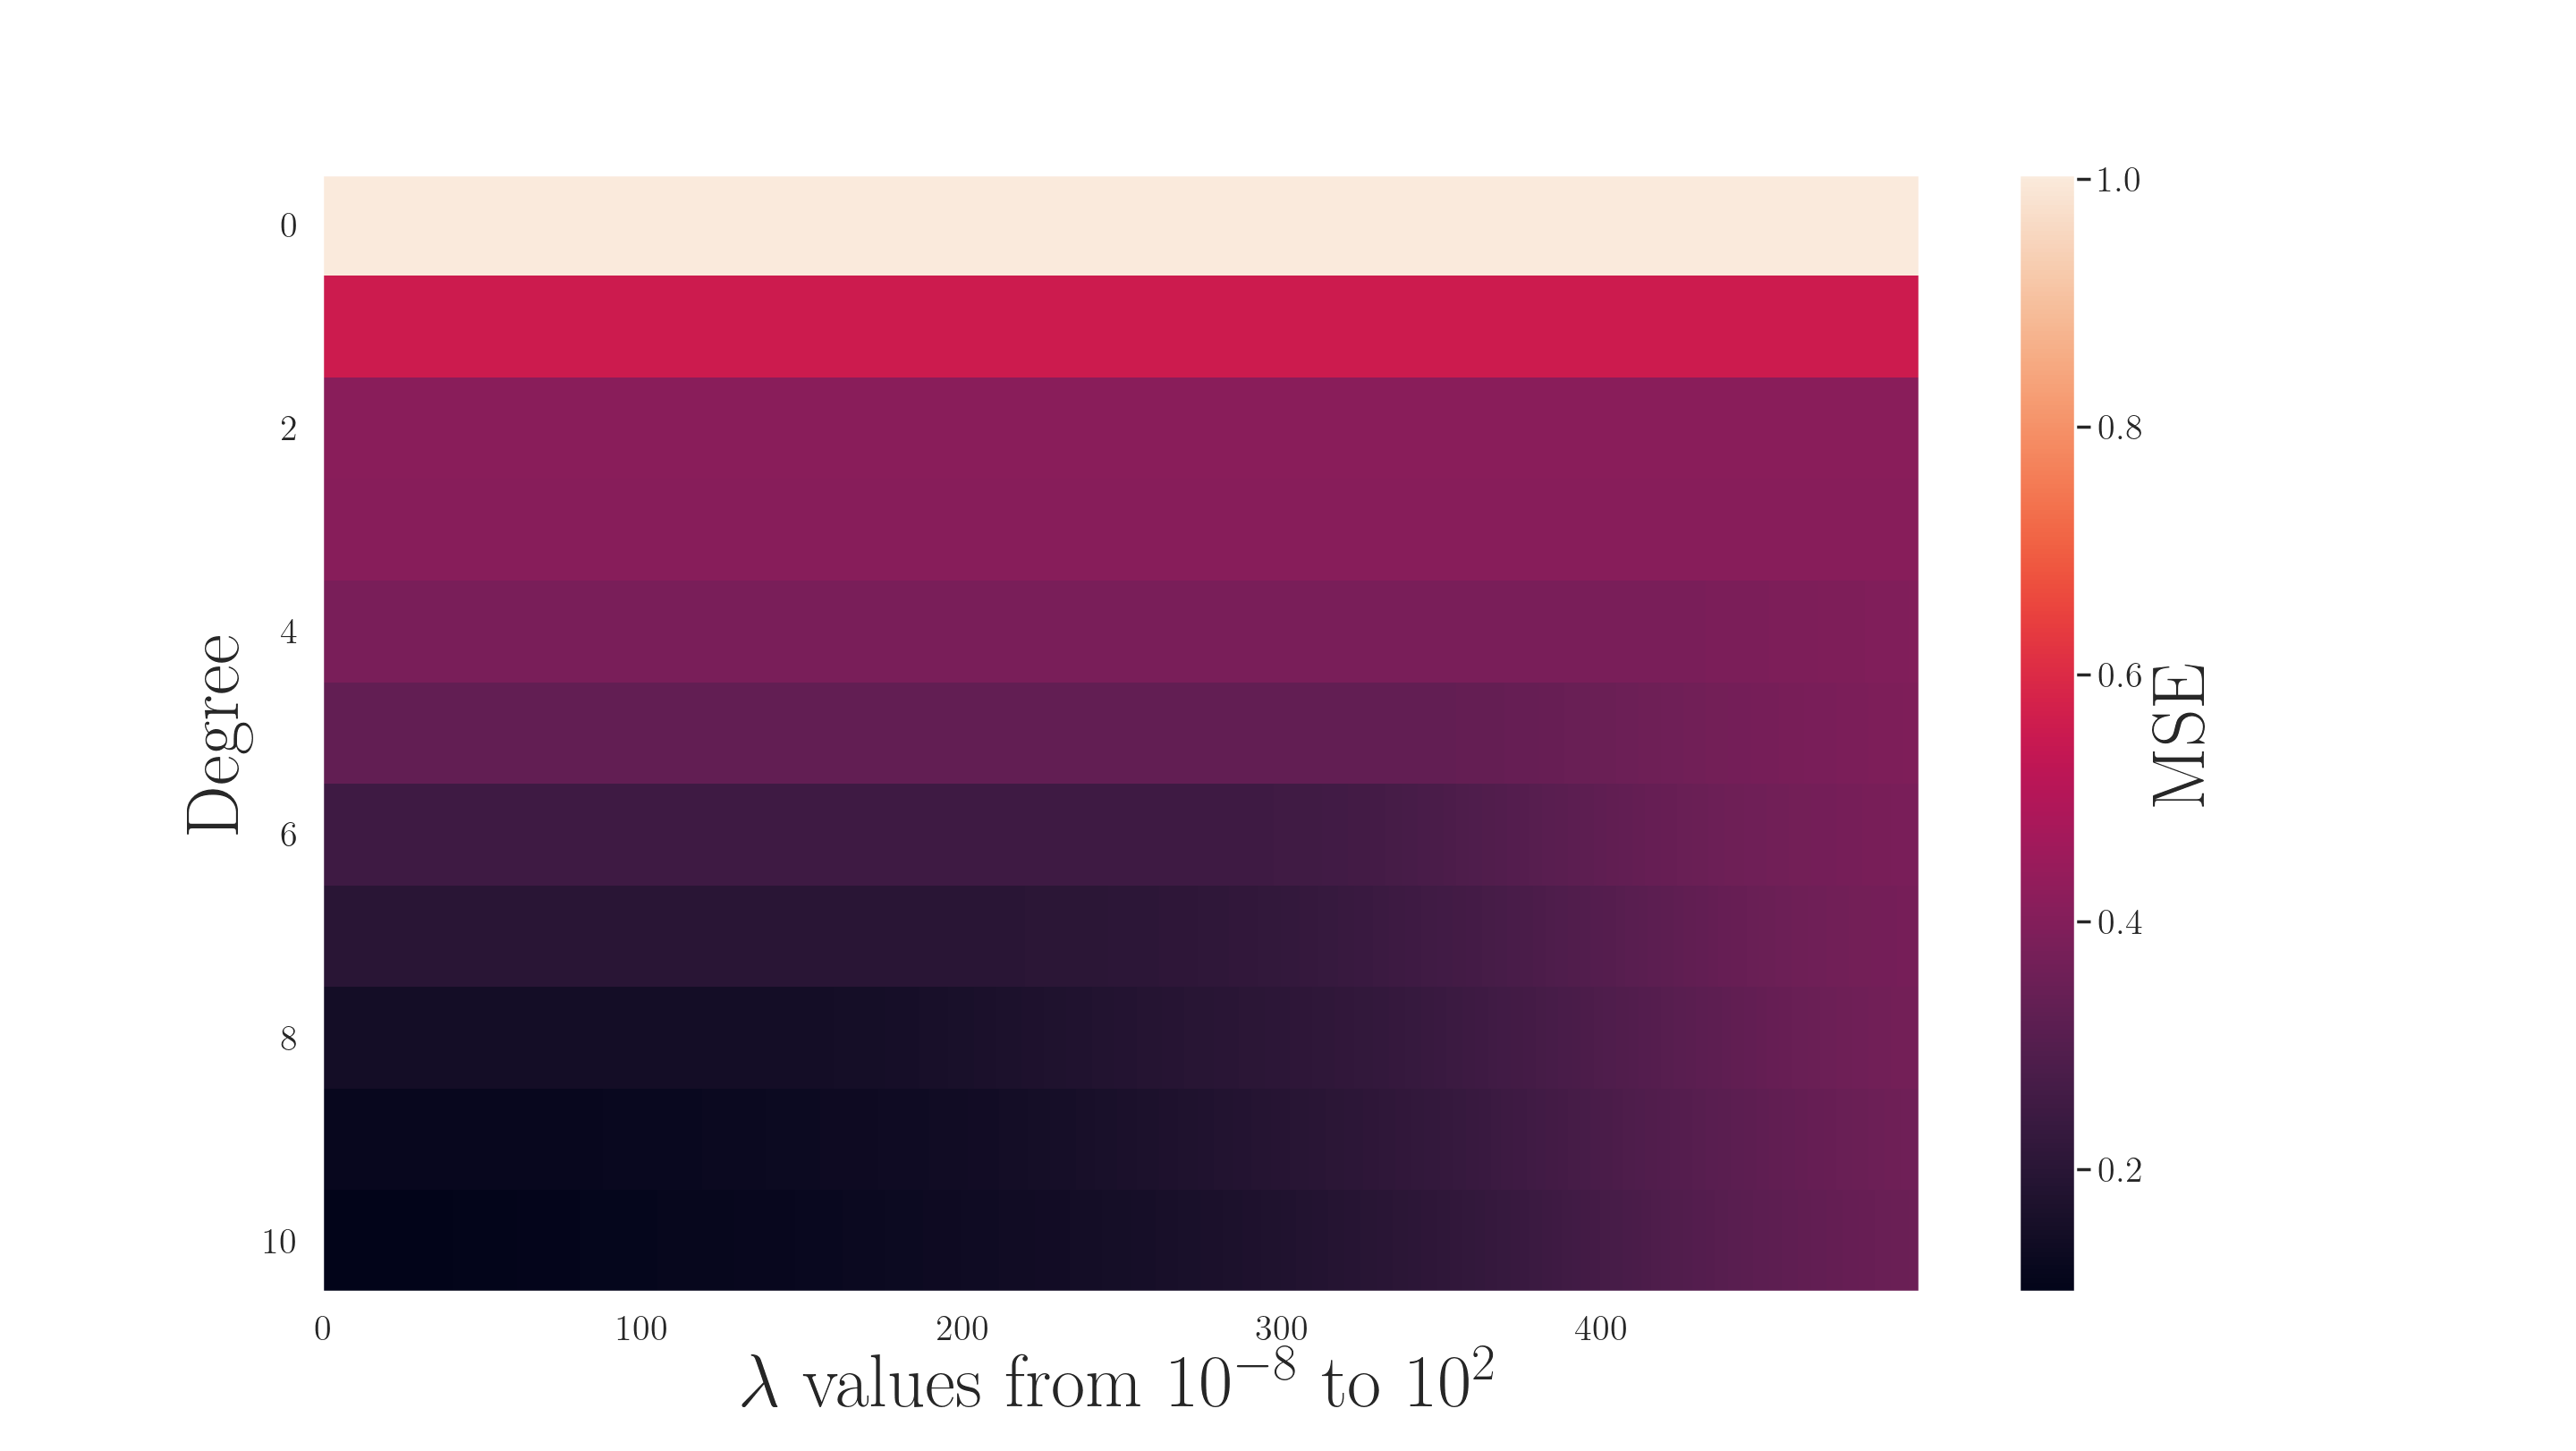
\includegraphics[width=\linewidth]{images/Figure_23.png}
	\caption{Heat map of the MSE for the test data, as a function of complexity and $lambda$ values.}
	\label{heat map Ridge Terrain data test}
\end{figure}
\noindent We also plotted the MSE and R2 score as a function of only complexity, where $\lambda$ was put to $\lambda = 10^{-5}$. The result are shown in figure \eqref{MSE Ridge terrain data}.
\begin{figure}[H]
	\centering
	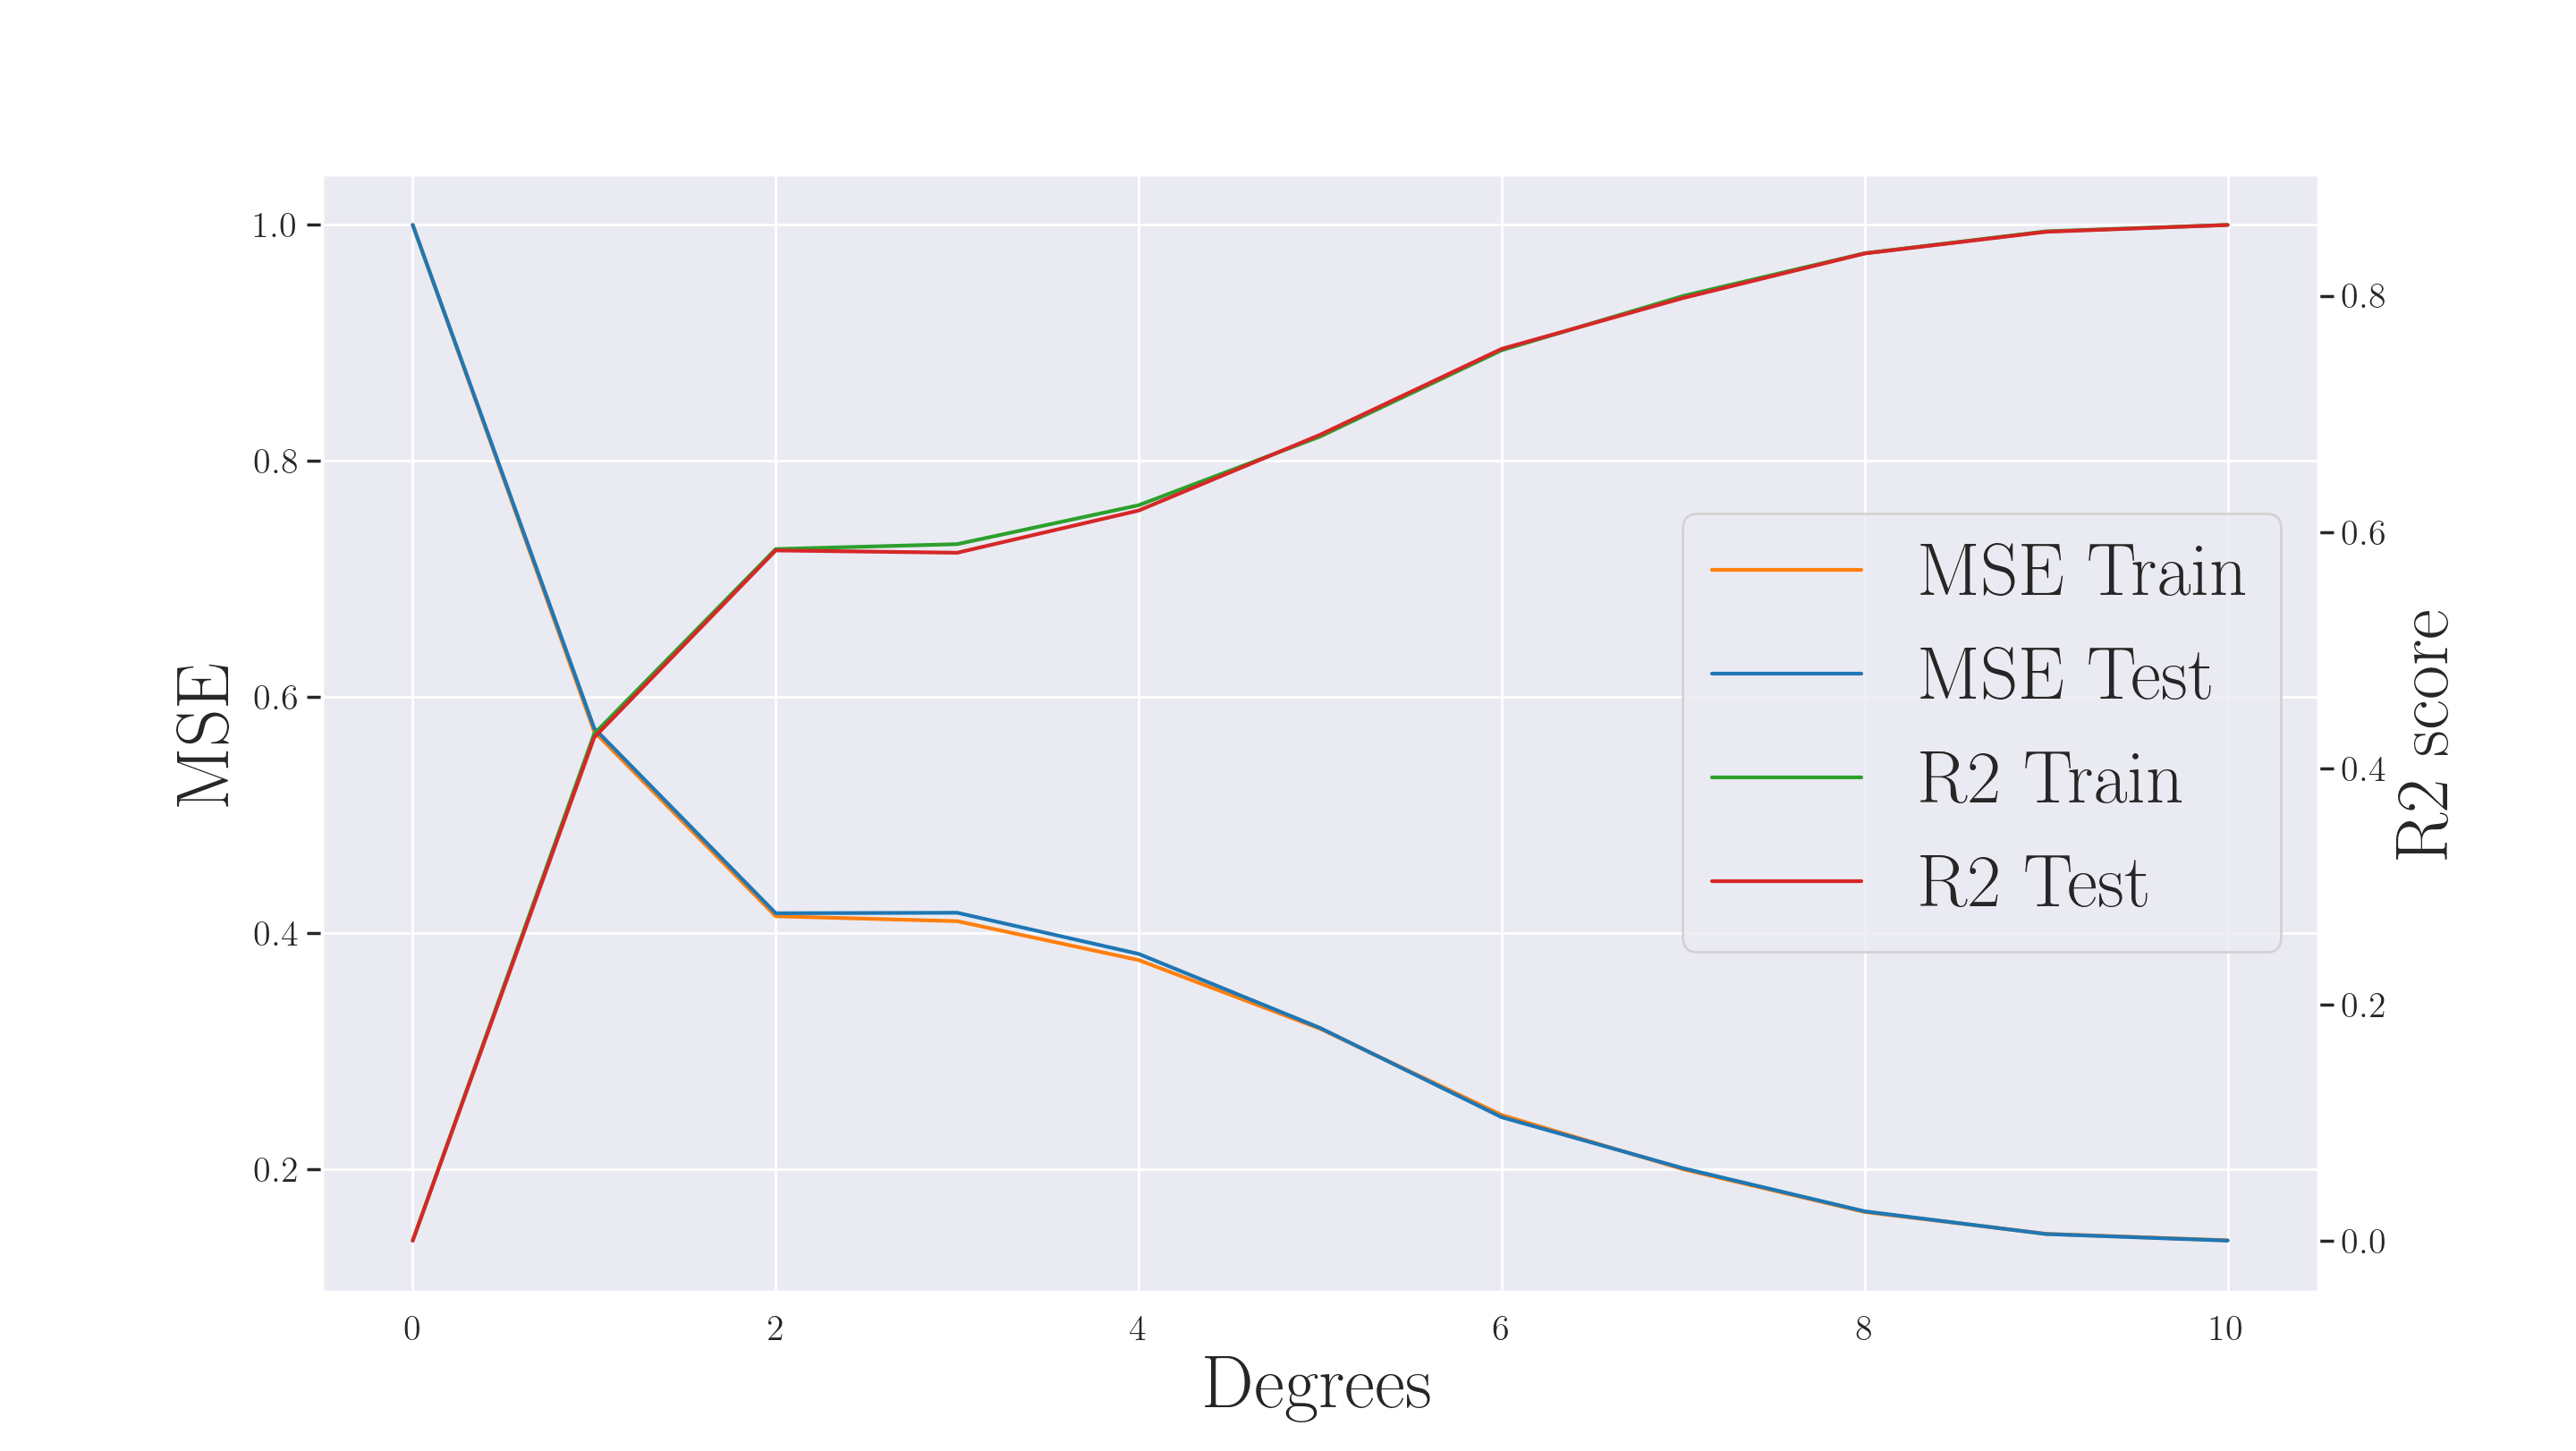
\includegraphics[width=\linewidth]{images/Figure_26.png}
	\caption{MSE and R2 score as a function of complexity with $\lambda = 10^{-5}$ for the terrain data modelled with Ridge regression. }
	\label{MSE Ridge terrain data}
\end{figure}
\noindent We then plotted the MSE for both OLS and Ridge with a lambda value of $10^{-5}$ in the same plot to see how these compered to each other. The plot is shown in figure \eqref{MSE OLS and Ridge}
\begin{figure}[H]
	\centering
	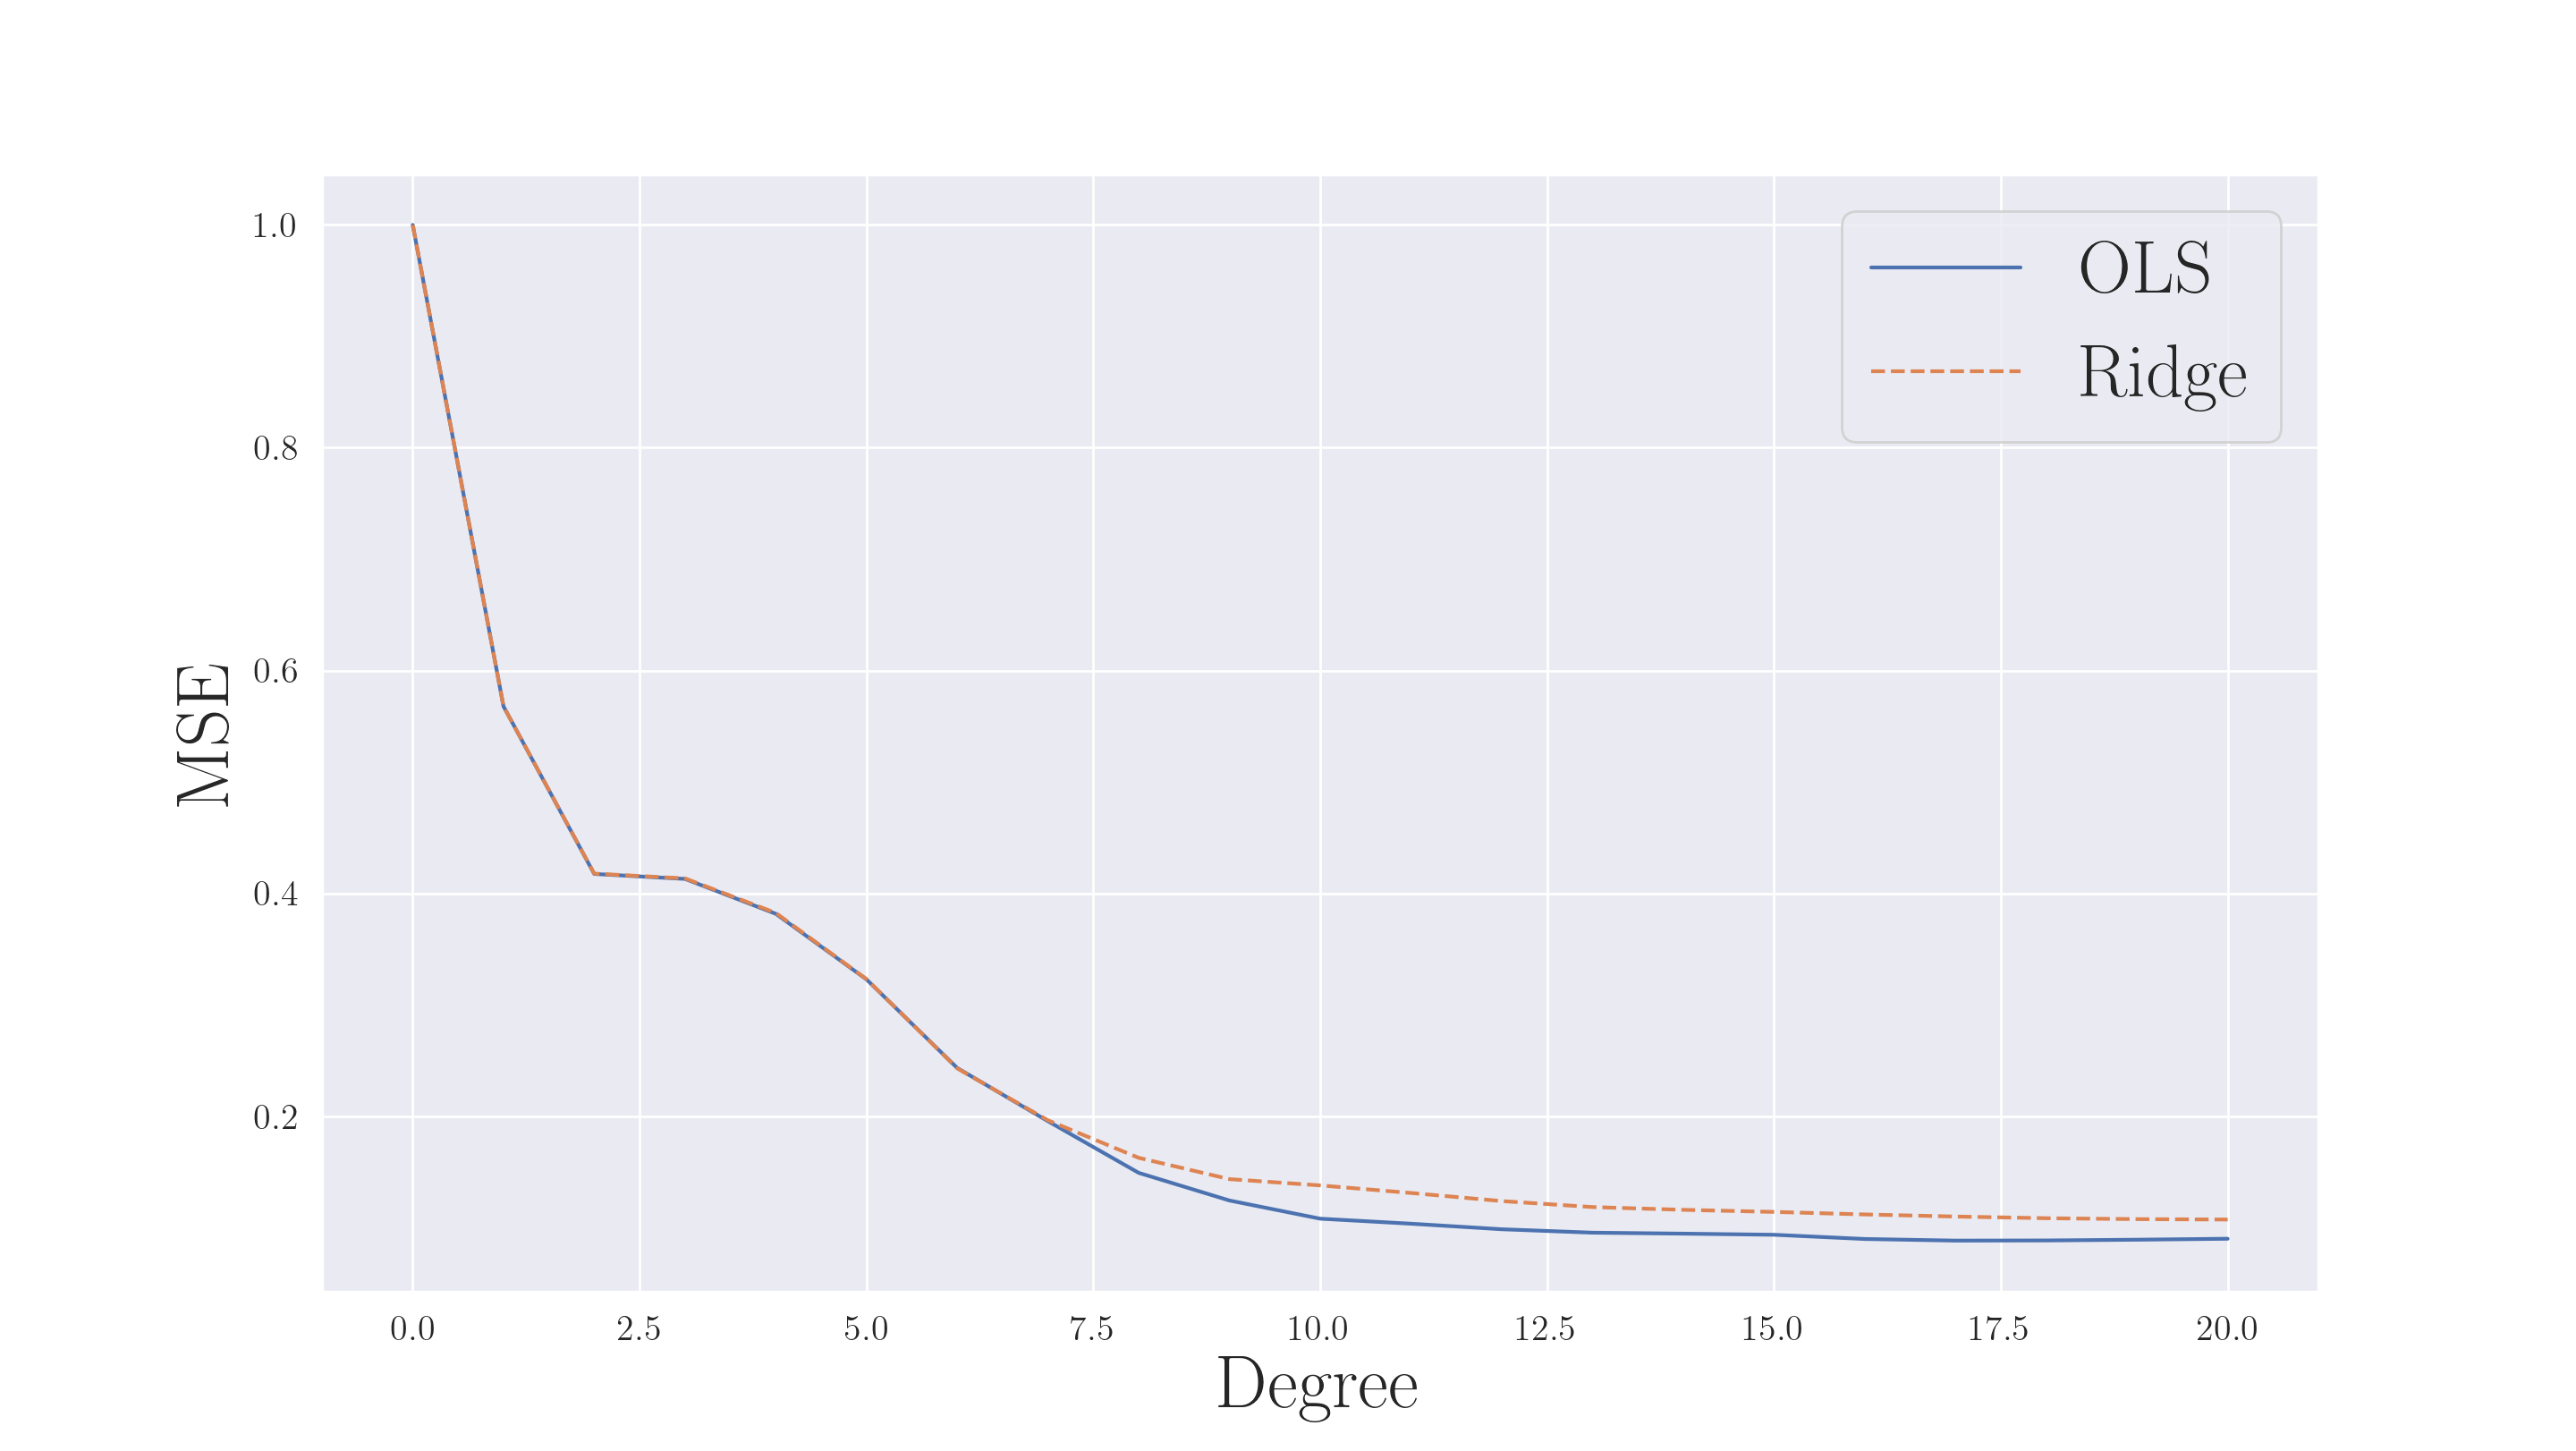
\includegraphics[width=\linewidth]{images/Figure_27.png}
	\caption{MSE as a function of complexity for both OLS and Ridge were Ridge is implemented with a $\lambda$ value of $10^{-5}$. }
	\label{MSE OLS and Ridge}
\end{figure}
%
\noindent The plot provided in figure \eqref{fig:cv_ridge_terrain} showcases the performance of Ridge Regression applied to real terrain data across various polynomial degrees and regularization strengths (denoted by $\lambda$).
%
\begin{figure}[H]
    \centering
    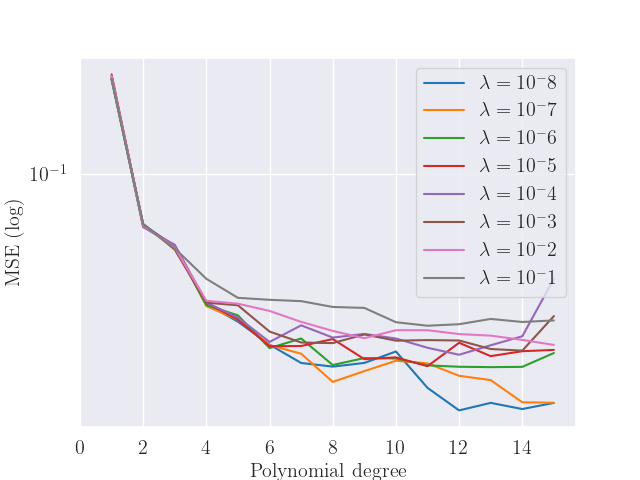
\includegraphics[width=\linewidth]{images/cv_ridge_terrain.png}
    \caption{MSE as a function of complexity for Ridge with terrain data, using cross validation with $k=5$.}
    \label{fig:cv_ridge_terrain}
\end{figure}

\subsubsection{LASSO}
\noindent Last we applied LASSO regression on the terrain data. Due to the time used to run this code the heat map is made out of 10 $\lambda$ values instead of 1000 as for Ridge. The heat map for both the training data and for test data is shown in figure \eqref{Heat map LASSO terrain training} and \eqref{Heat map LASSO terrain testing}. 
\begin{figure}[H]
	\centering
	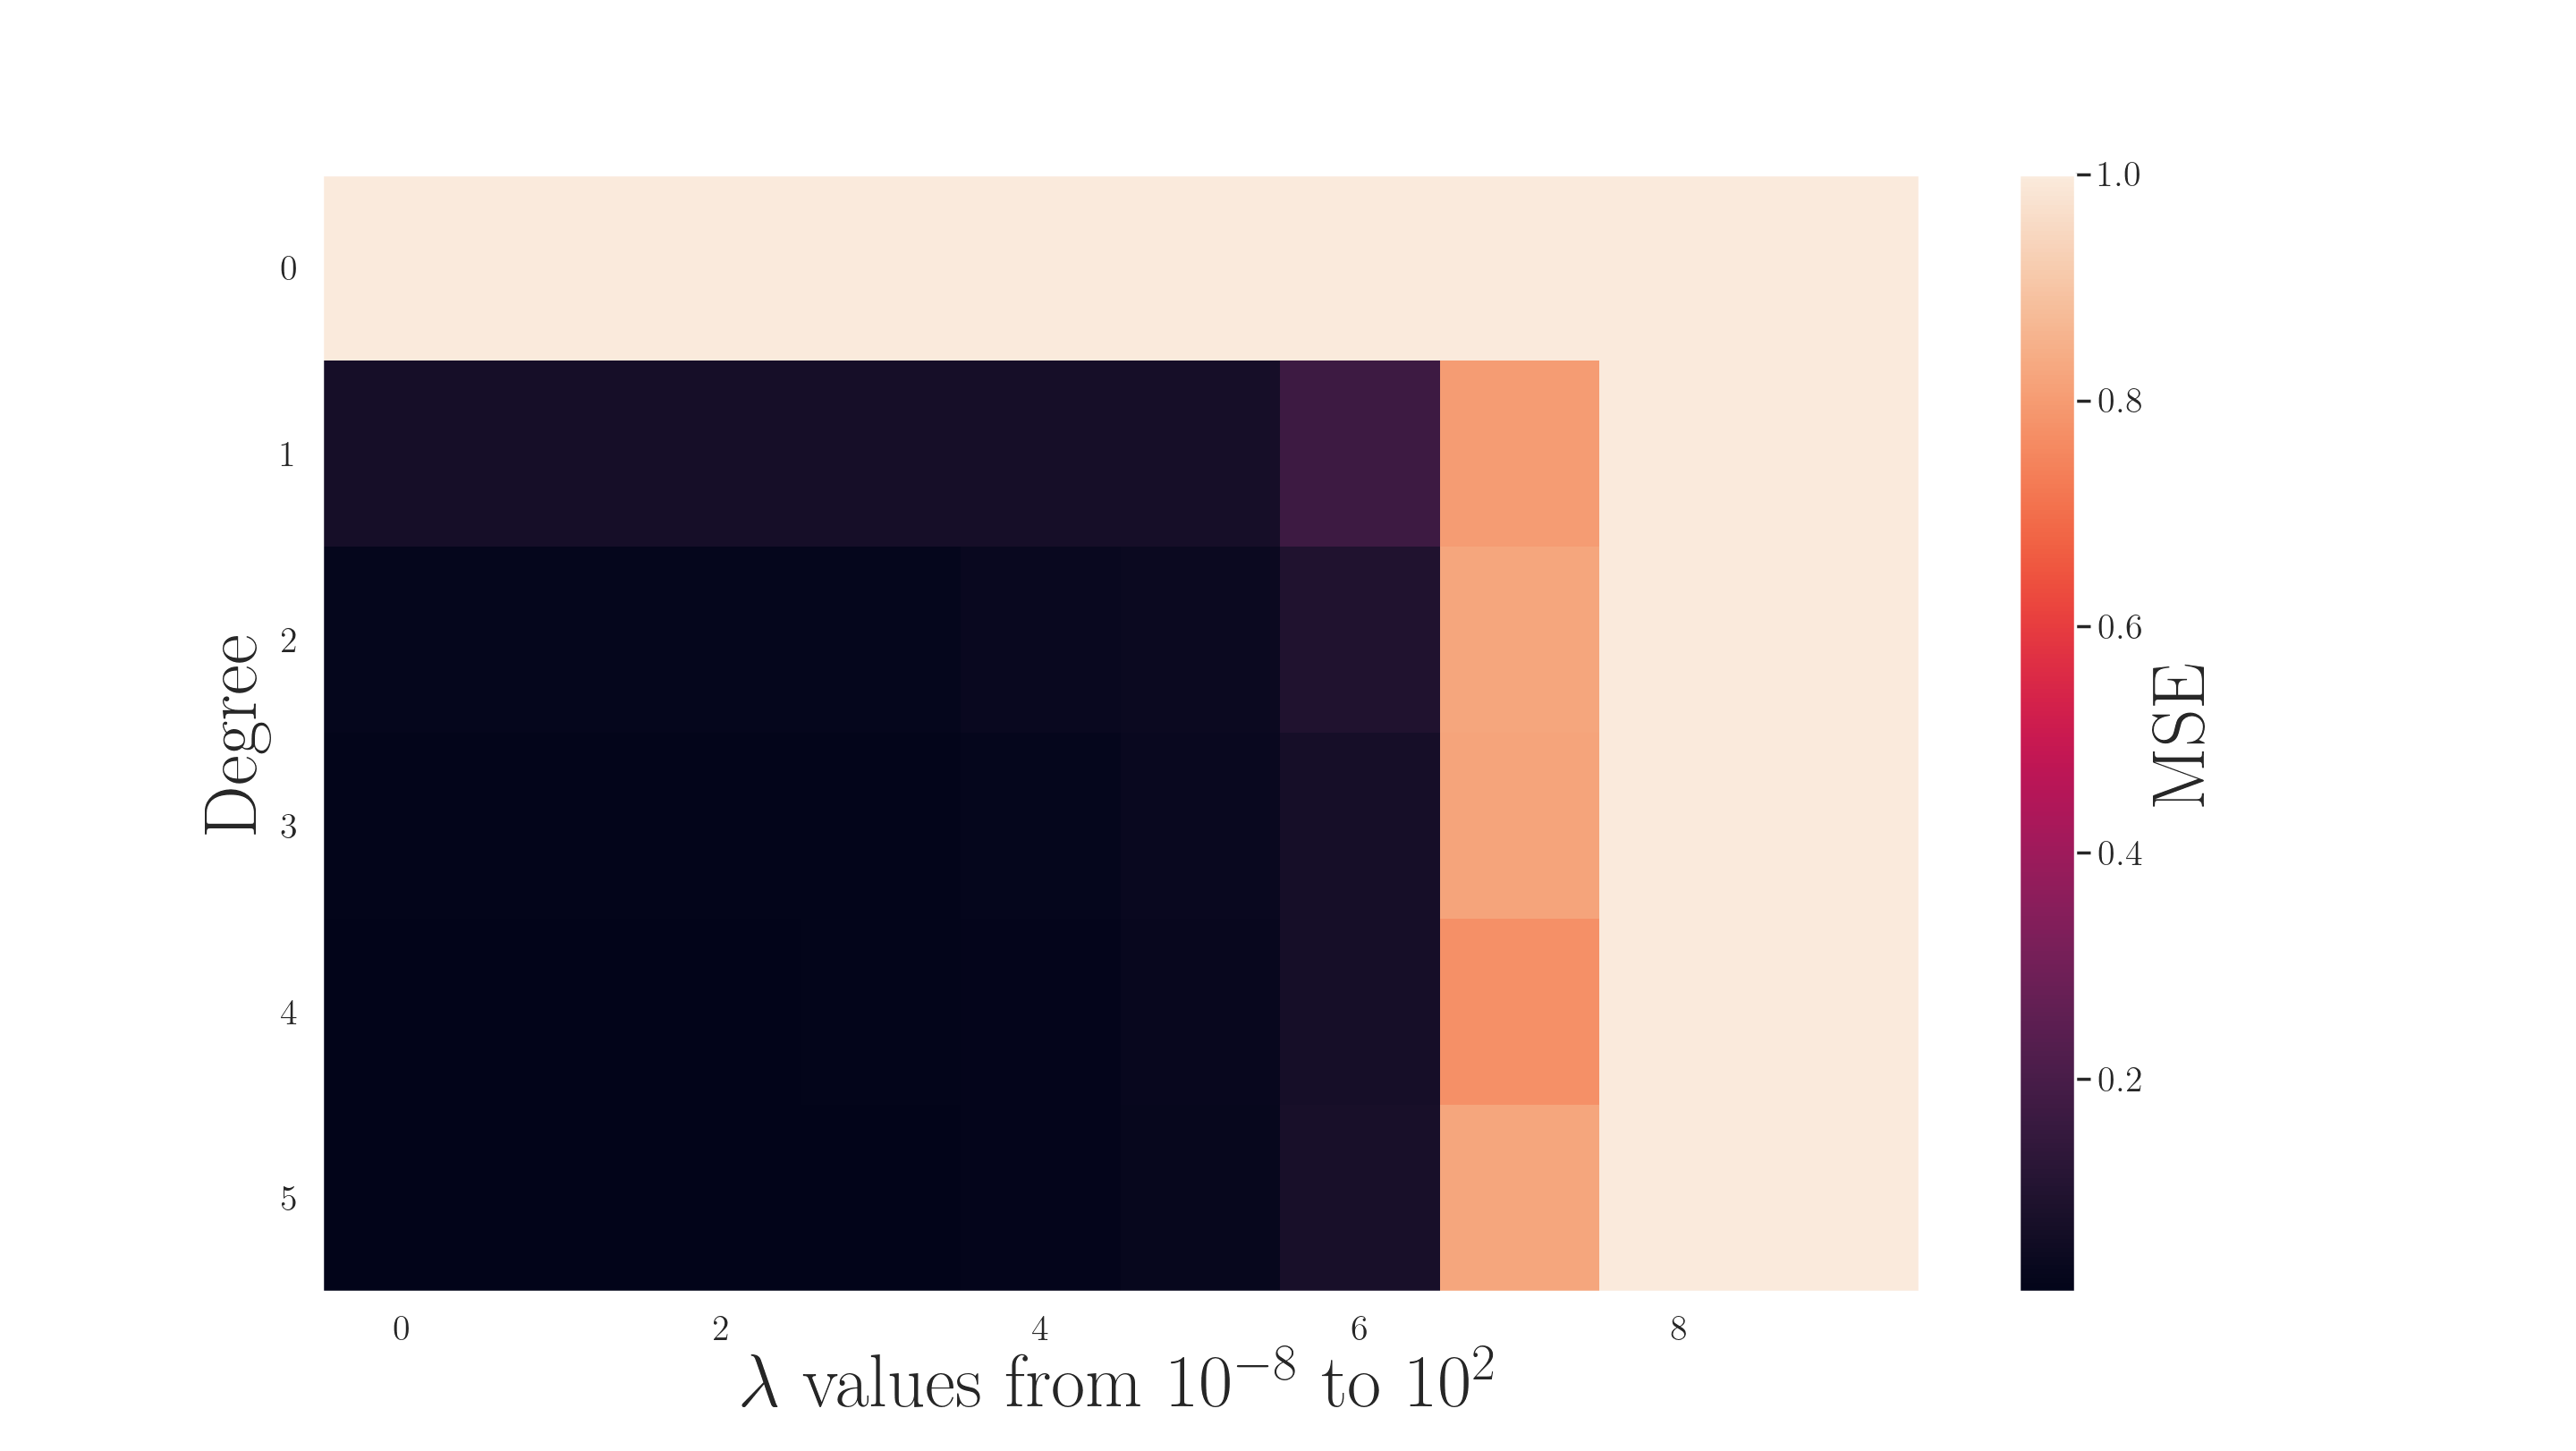
\includegraphics[width=\linewidth]{images/Figure_24.png}
	\caption{Heat map of the MSE for the training data, as a function of complexity and $lambda$ values for LASSO regression.}
	\label{Heat map LASSO terrain training}
\end{figure}
\begin{figure}[H]
	\centering
	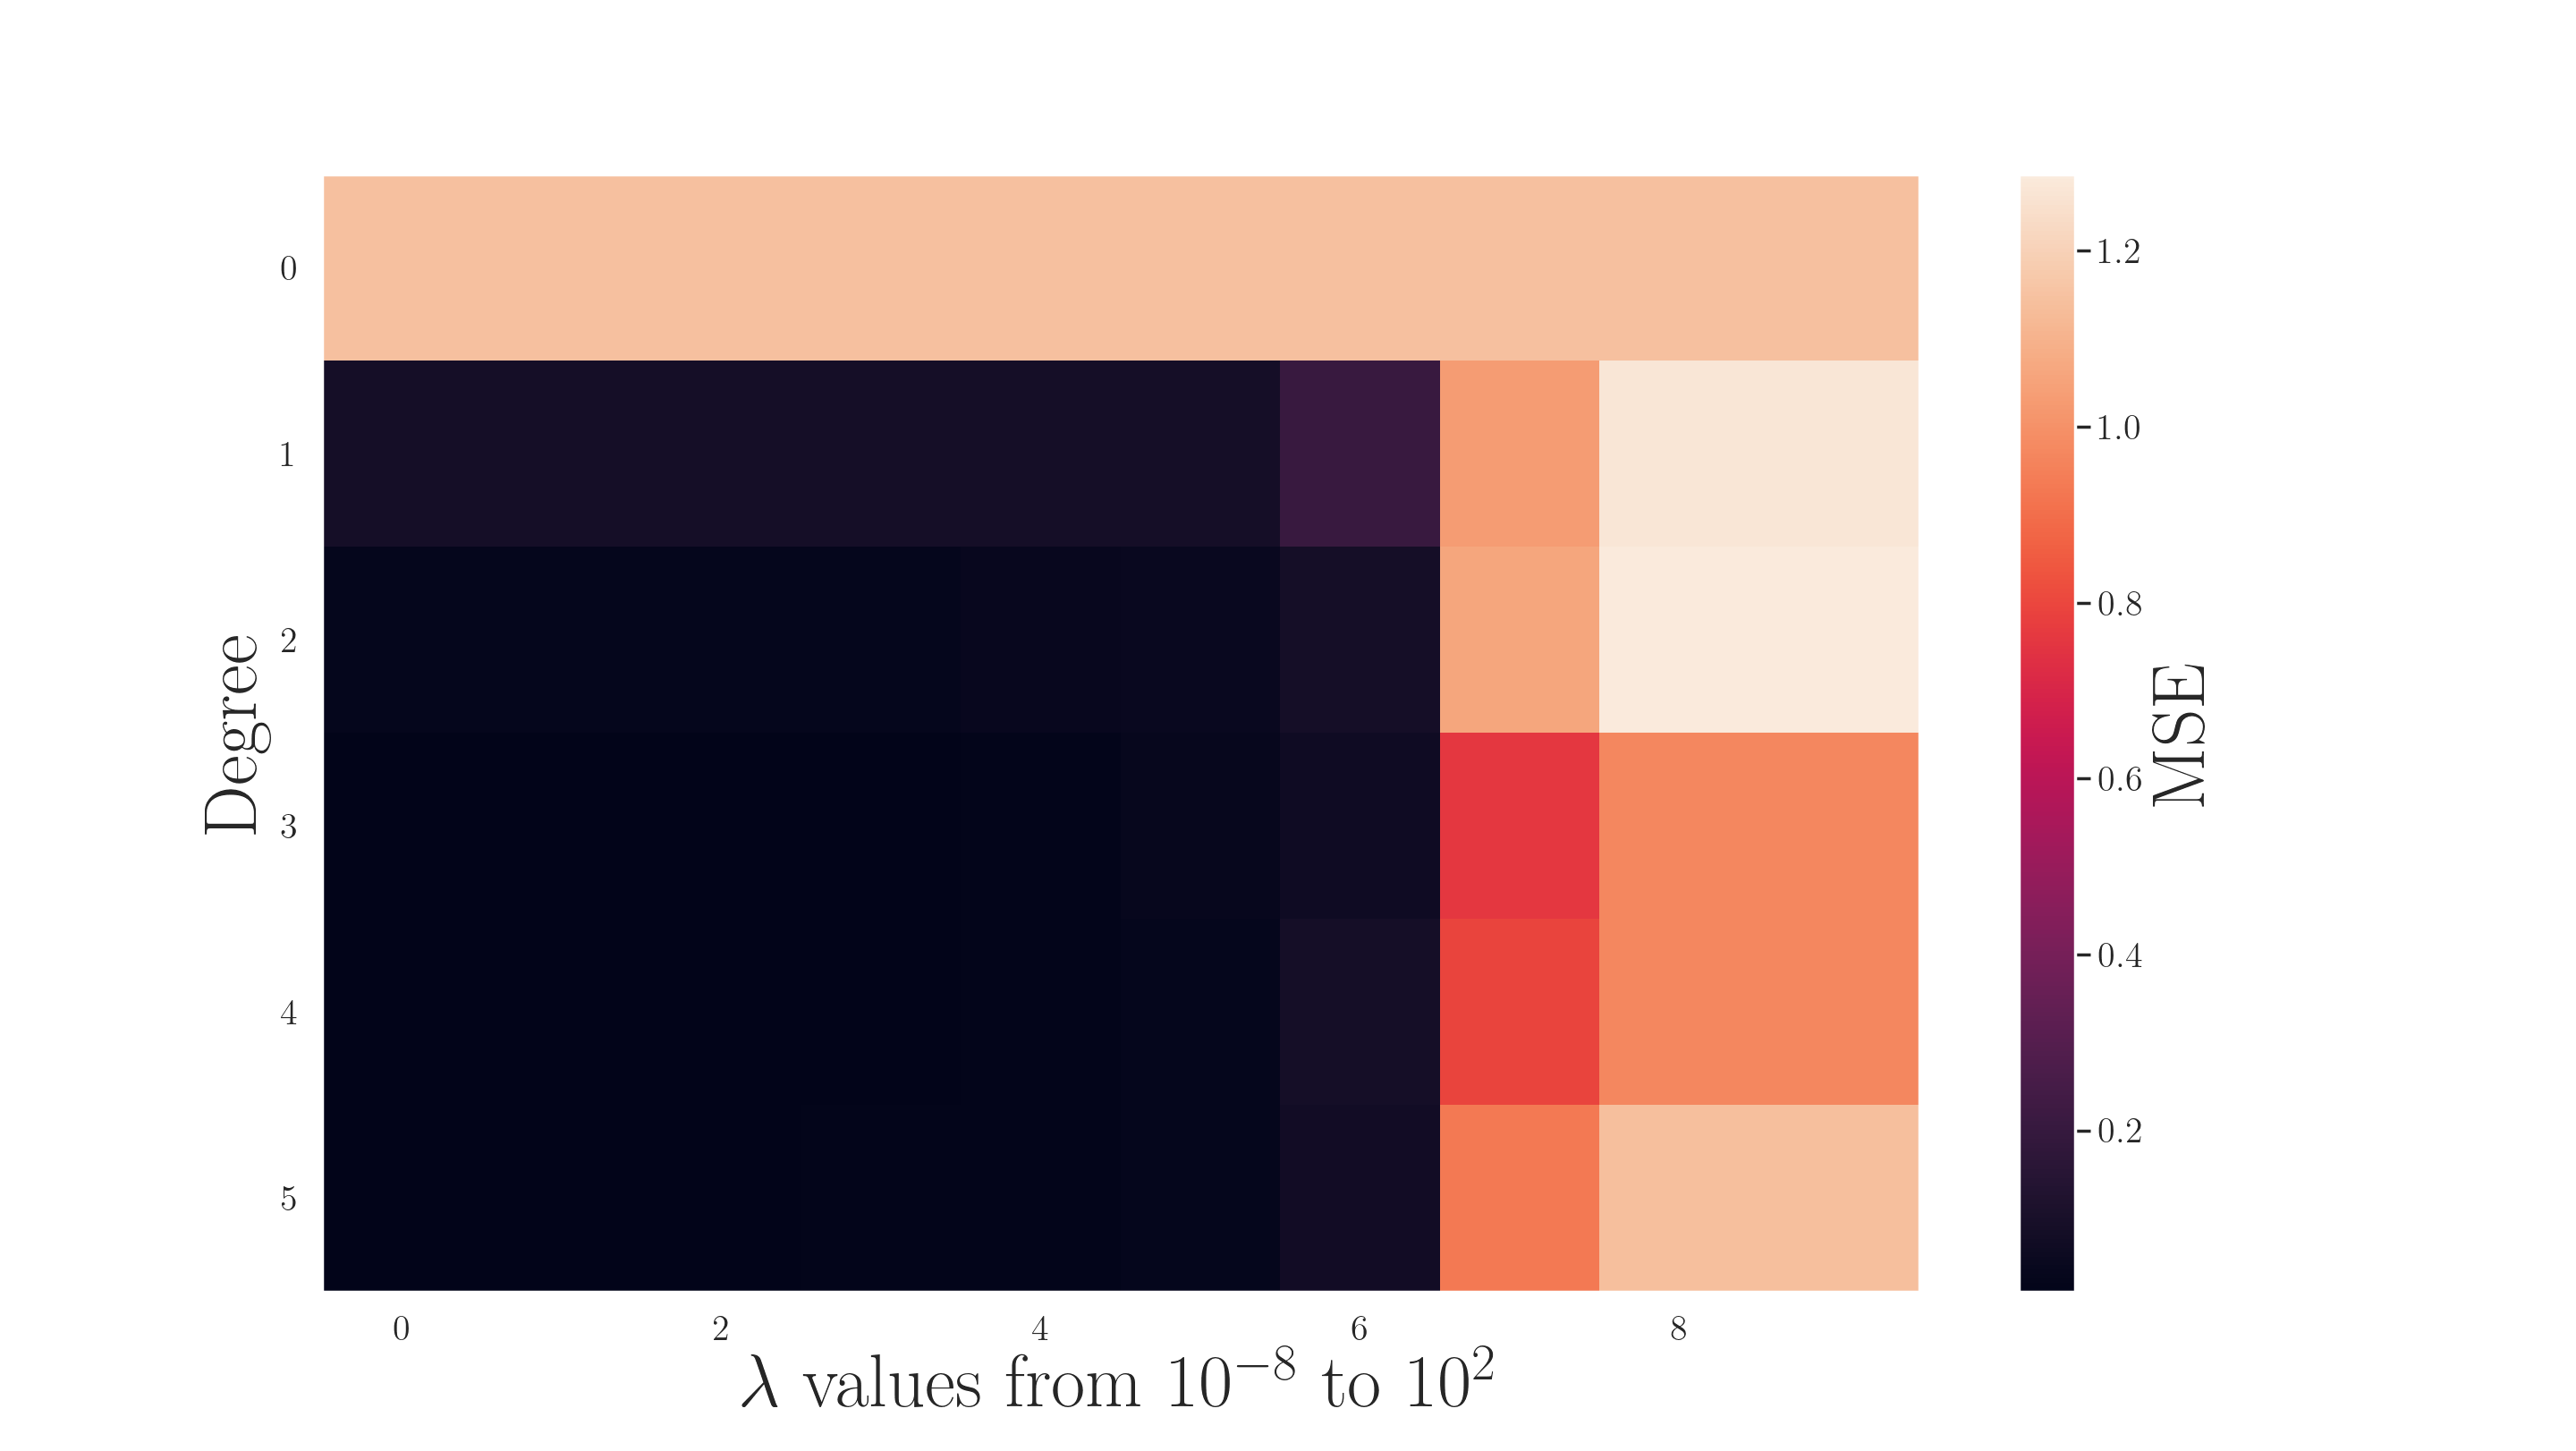
\includegraphics[width=\linewidth]{images/Figure_25.png}
	\caption{Heat map of the MSE for the test data, as a function of complexity and $lambda$ values for LASSO regression.}
	\label{Heat map LASSO terrain testing}
\end{figure}
%
\noindent We then also plotted the MSE and R2 score as a function of only complexity, where $\lambda$ was put to $\lambda = 10^{-5}$. The result are shown in figure \eqref{MSE LASSO terrain data}.
\begin{figure}[H]
	\centering
	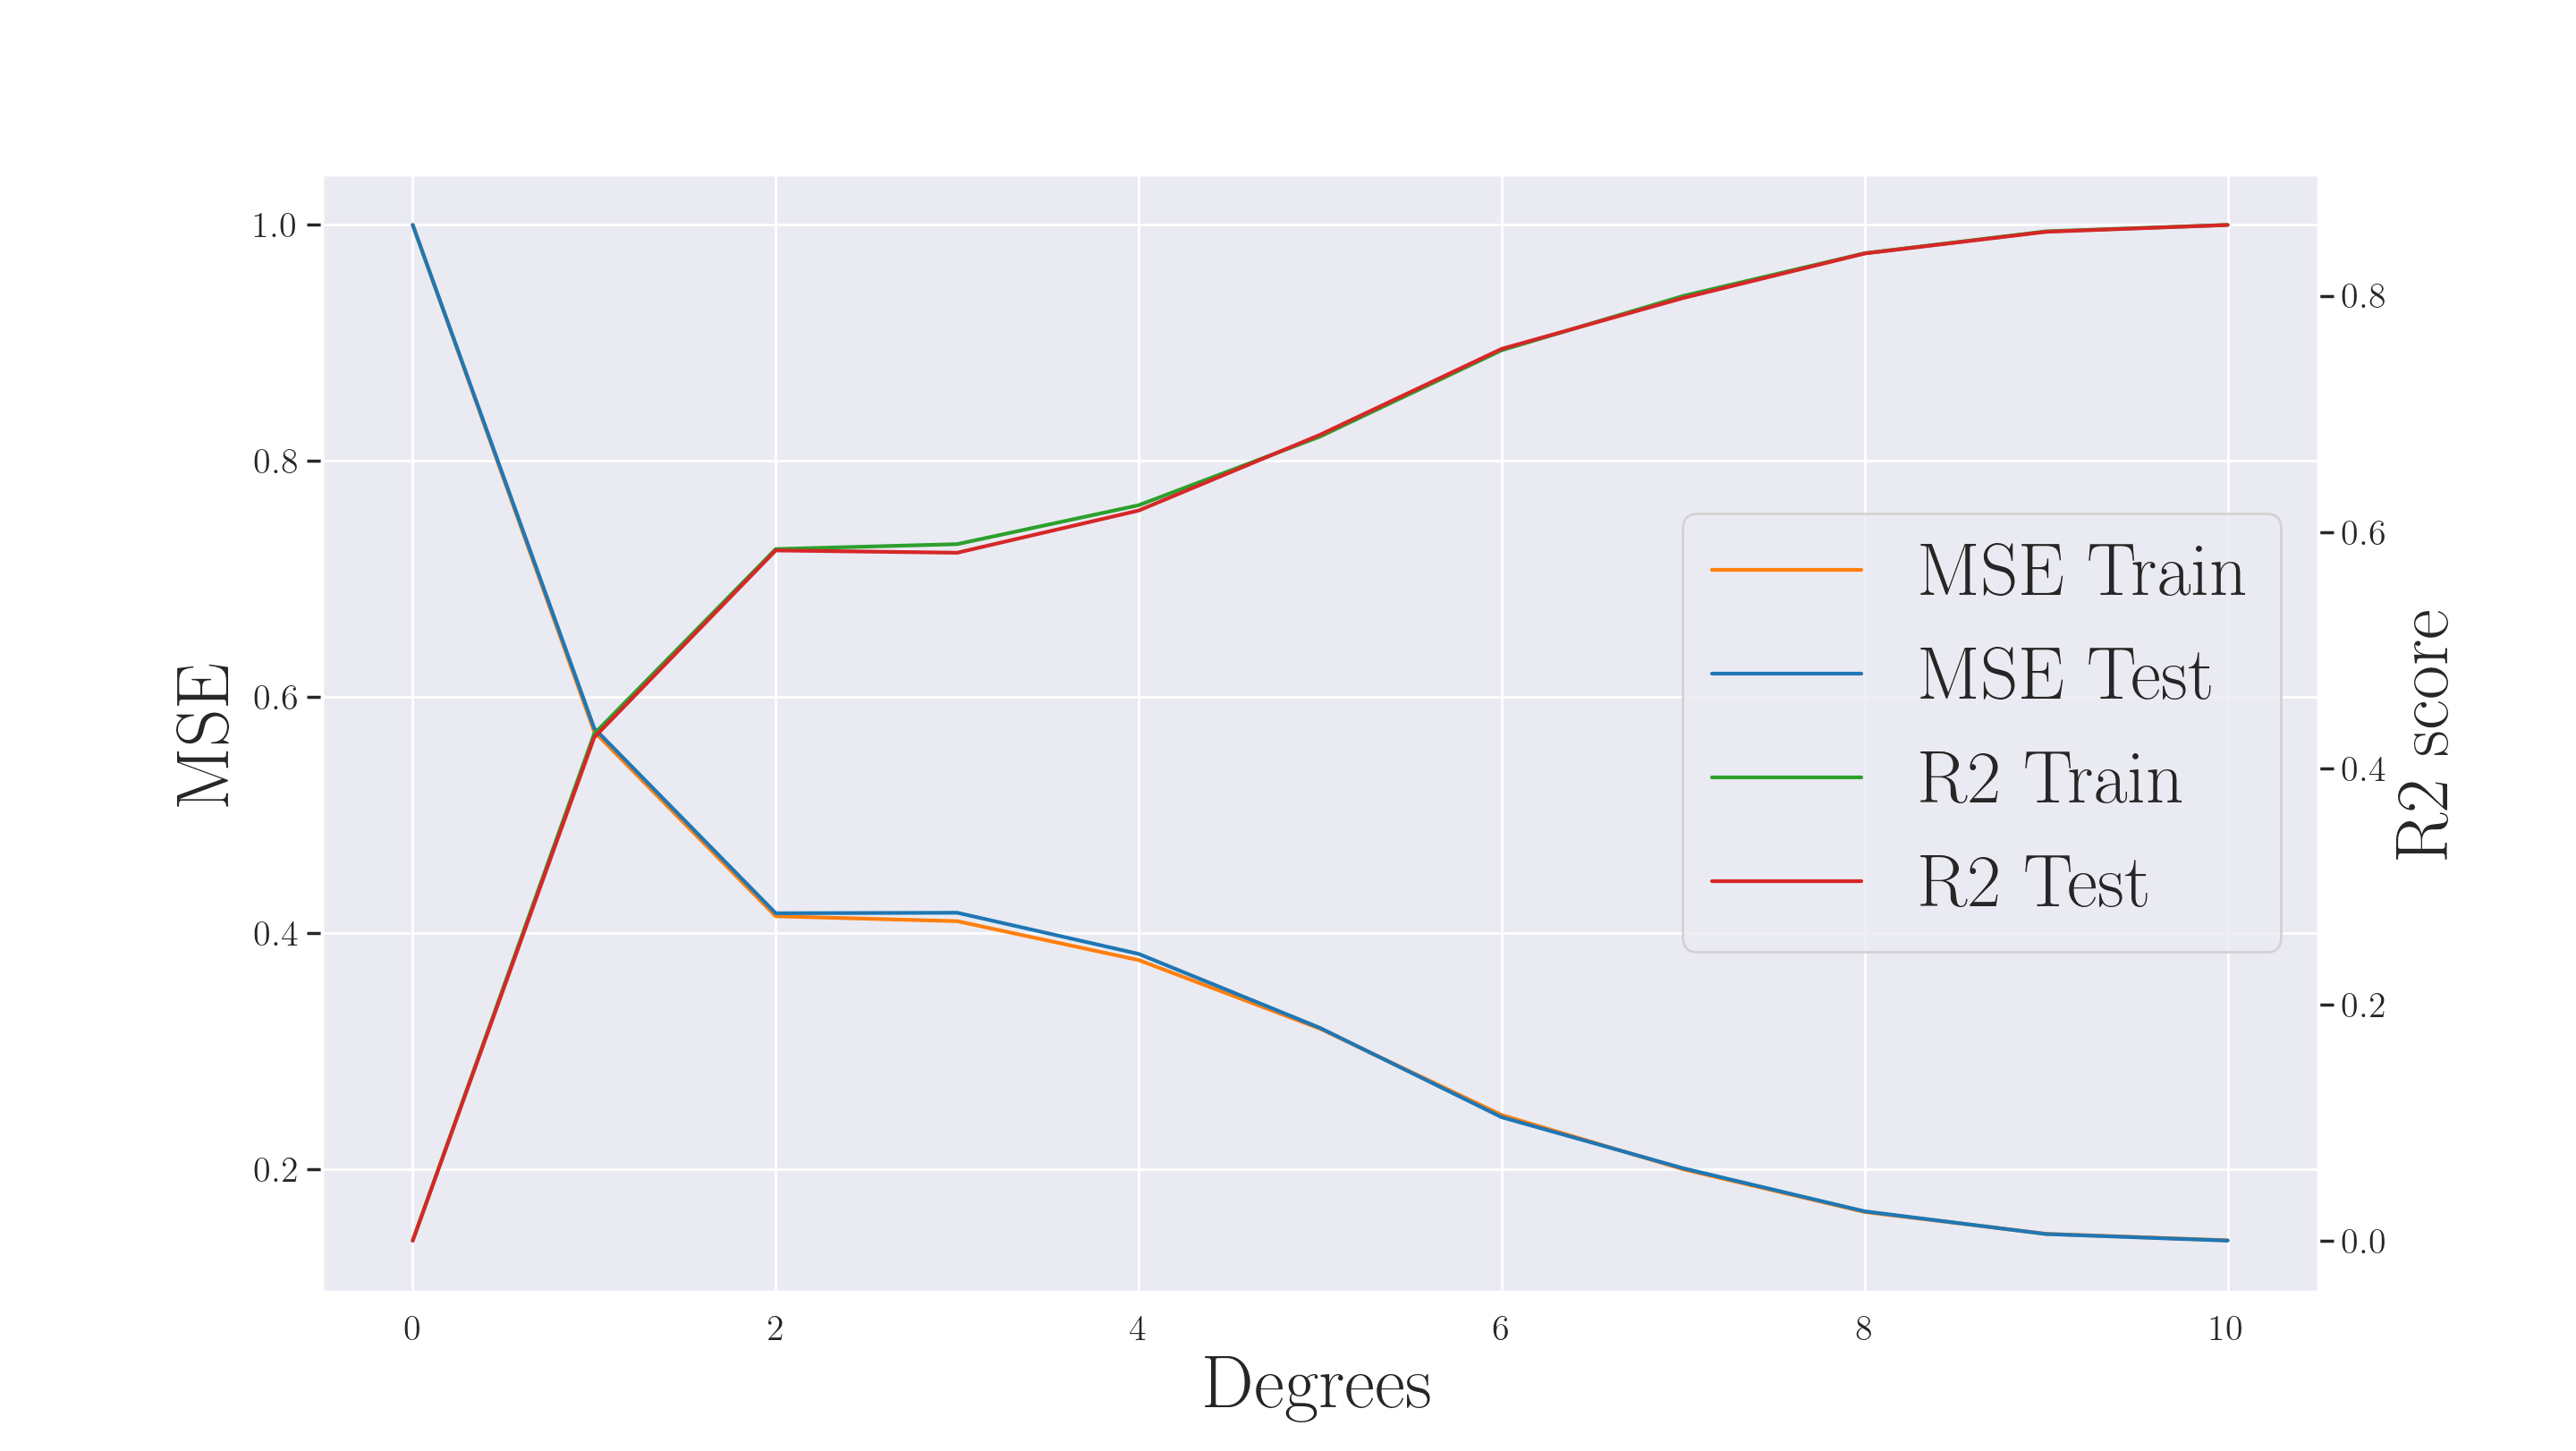
\includegraphics[width=\linewidth]{images/Figure_26.png}
	\caption{MSE and R2 score as a function of complexity with $\lambda = 10^{-5}$ for the terrain data modelled with LASSO regression. }
	\label{MSE LASSO terrain data}
\end{figure}
%
\noindent We then plotted the MSE as a function of complexity for both OLS, Ridge and LASSO to compere the three regression methods for the terrain data. The plot is shown in figure \eqref{MSE for OLS, Ridge and LASSO}.
\begin{figure}[H]
	\centering
	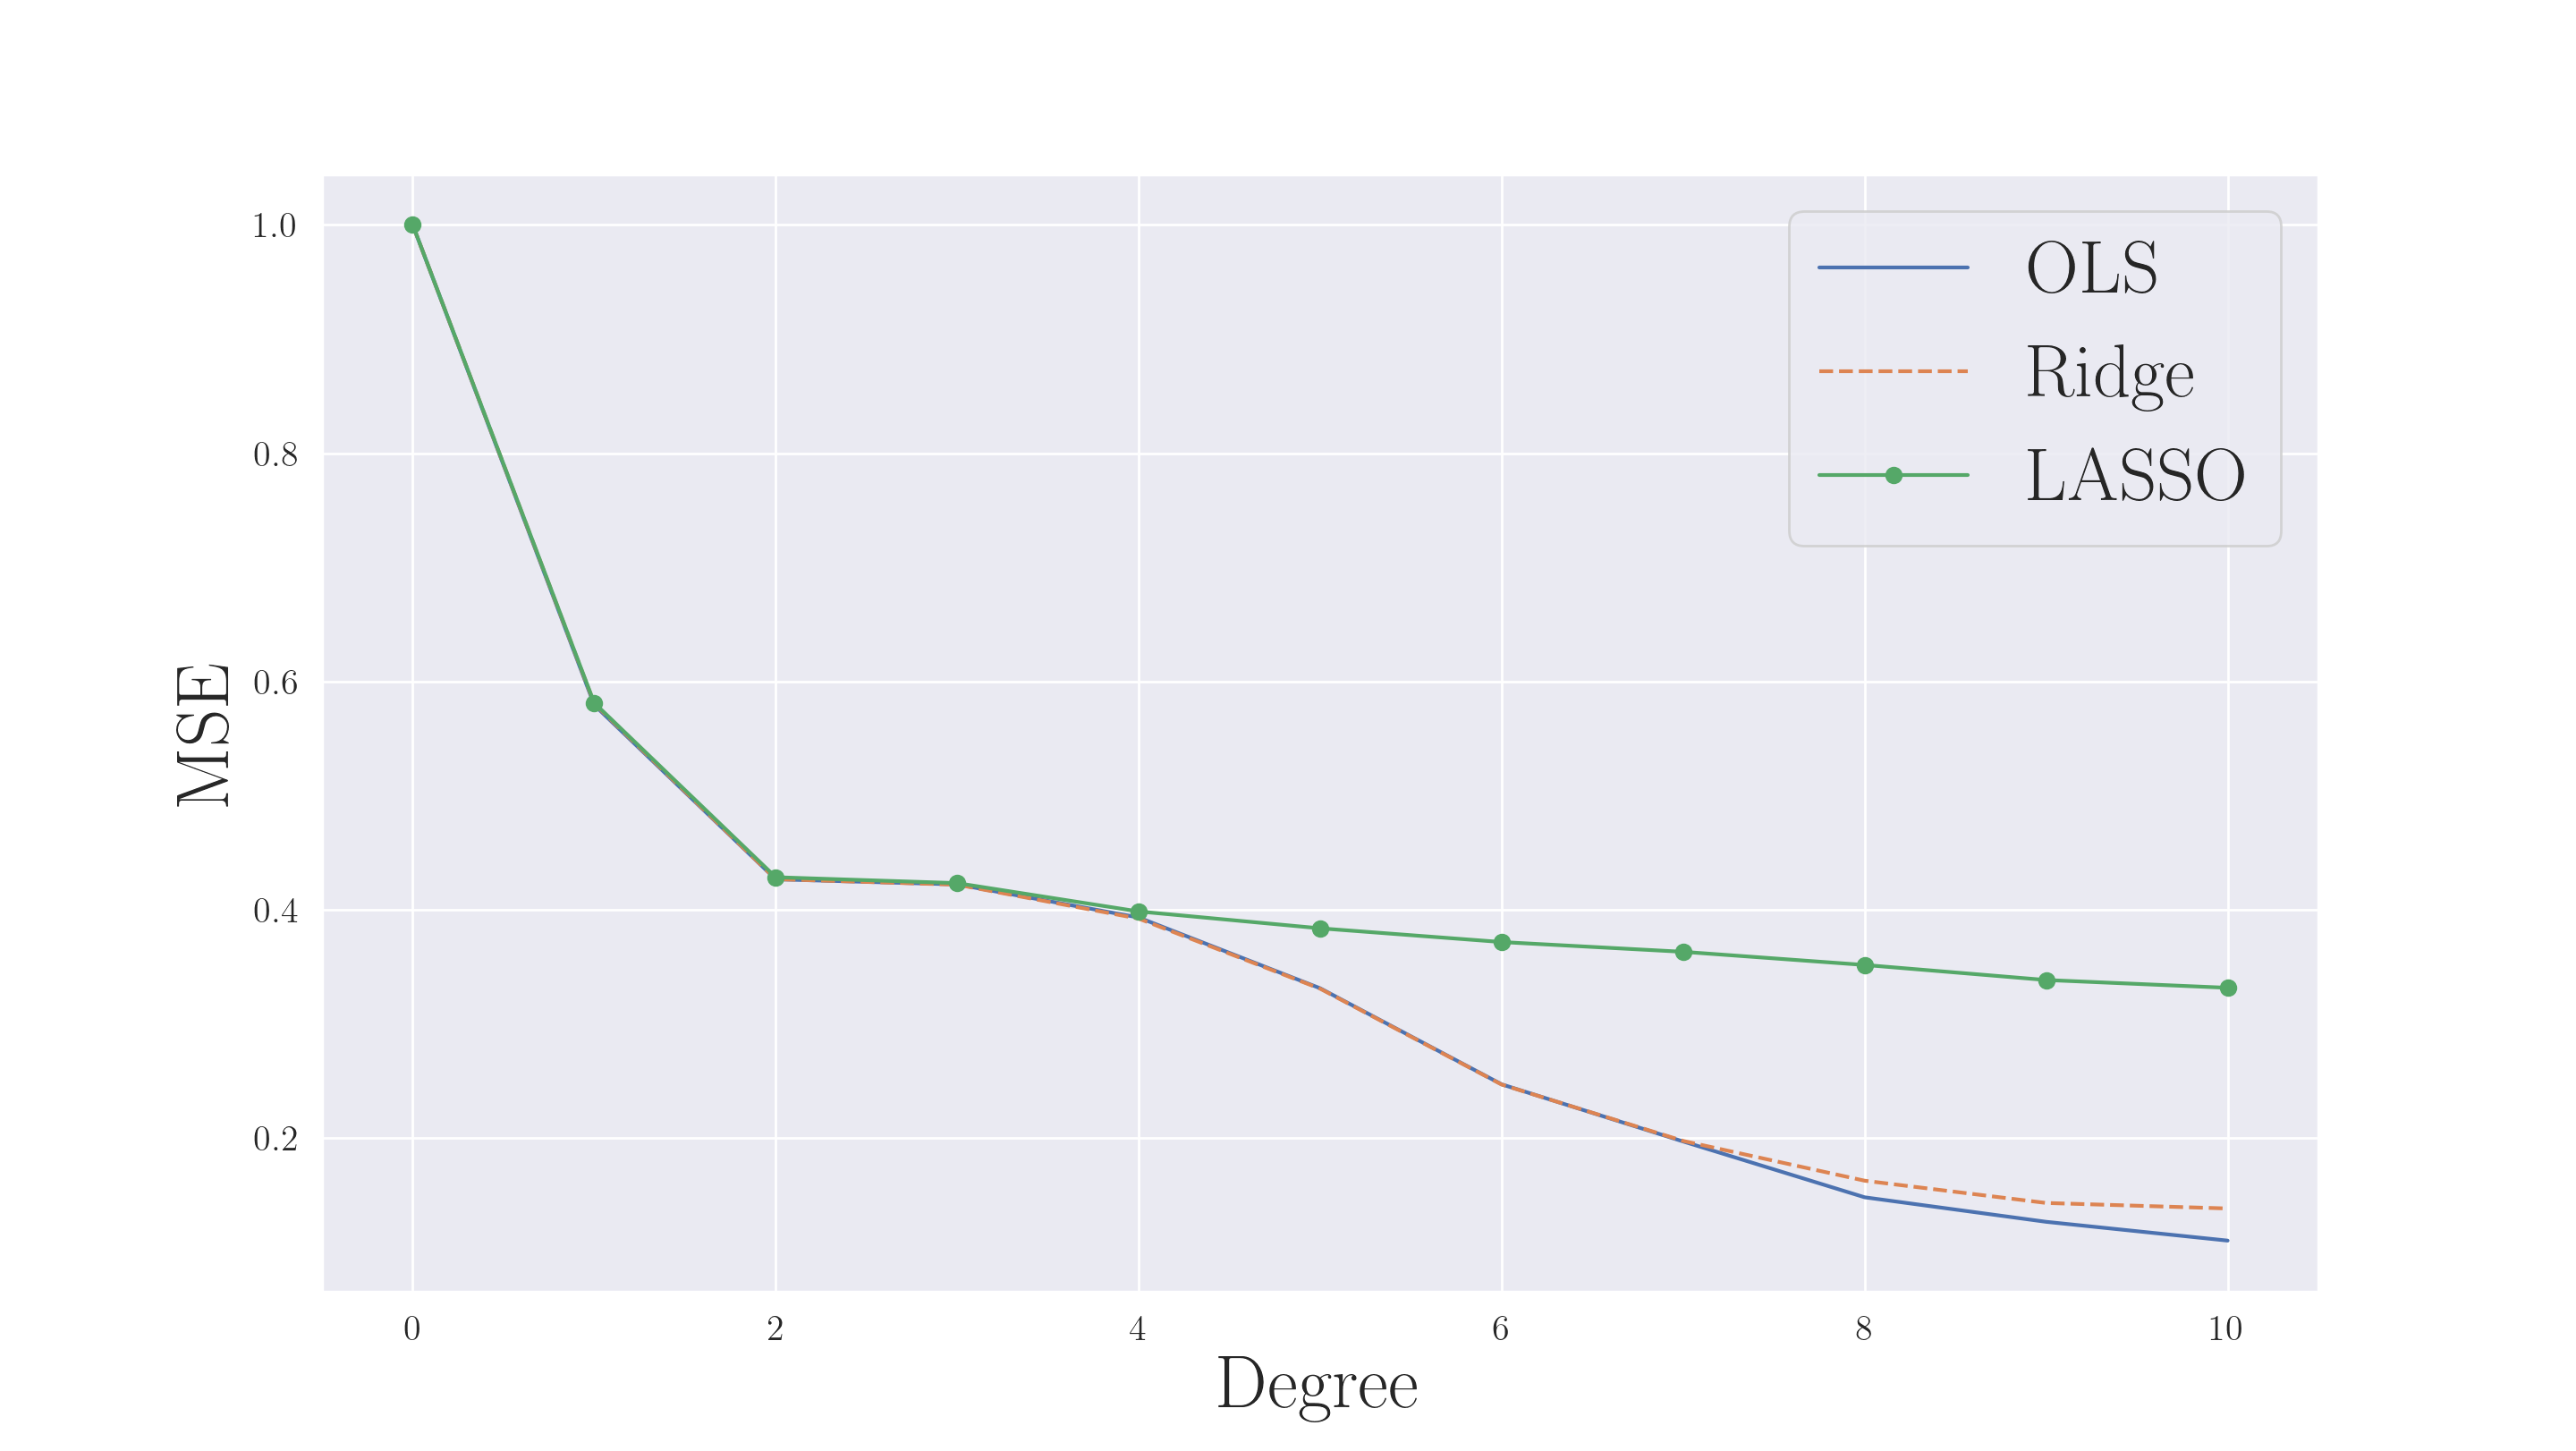
\includegraphics[width=\linewidth]{images/Figure_28.png}
	\caption{MSE as a function of complexity for both OLS, Ridge and LASSO were Ridge and LASSO are implemented with a $\lambda$ value of $10^{-5}$. }
	\label{MSE for OLS, Ridge and LASSO}
\end{figure}
%
\noindent Lastly the plotted in figure \eqref{fig:cv_lasso_terrain} showcases the performance of LASSO Regression applied to real terrain data across various polynomial degrees and regularization strengths (denoted by $\lambda$). 
%
\begin{figure}[H]
    \centering
    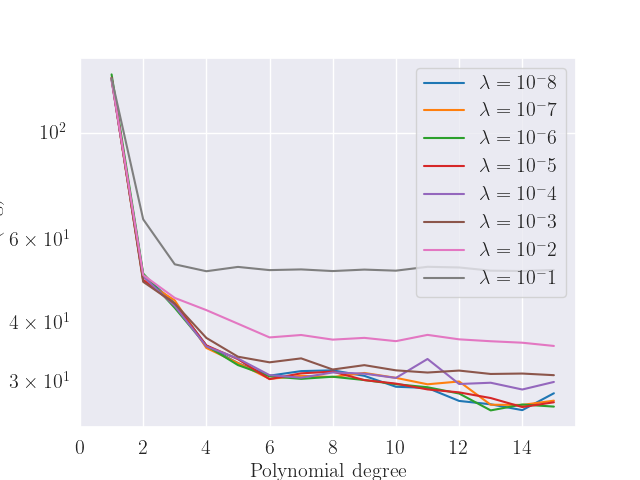
\includegraphics[width=\linewidth]{images/cv_lasso_real.png}
    \caption{MSE as a function of complexity for LASSO with terrain data, using cross validation with $k=5$.}
    \label{fig:cv_lasso_terrain}
\end{figure}

%
\section{Discussion}
\thispagestyle{plain}
\subsection{The Franke function}
\noindent It was stated in the project description that we should use a noise that was given by the normal distribution $\mathcal{N}(0,1)$. What we found was that since the Franke Function when plotted for $x$ and $y$ in the range between $0$ and $1$ the maximal value of the Franke function becomes around $1.4$. When plotted with noise that had values
between $0$ and $1$ the plot of the Franke function becomes unrecognizable as shown in figure \eqref{franke noise 1}. 
\begin{figure}[H]
	\centering
	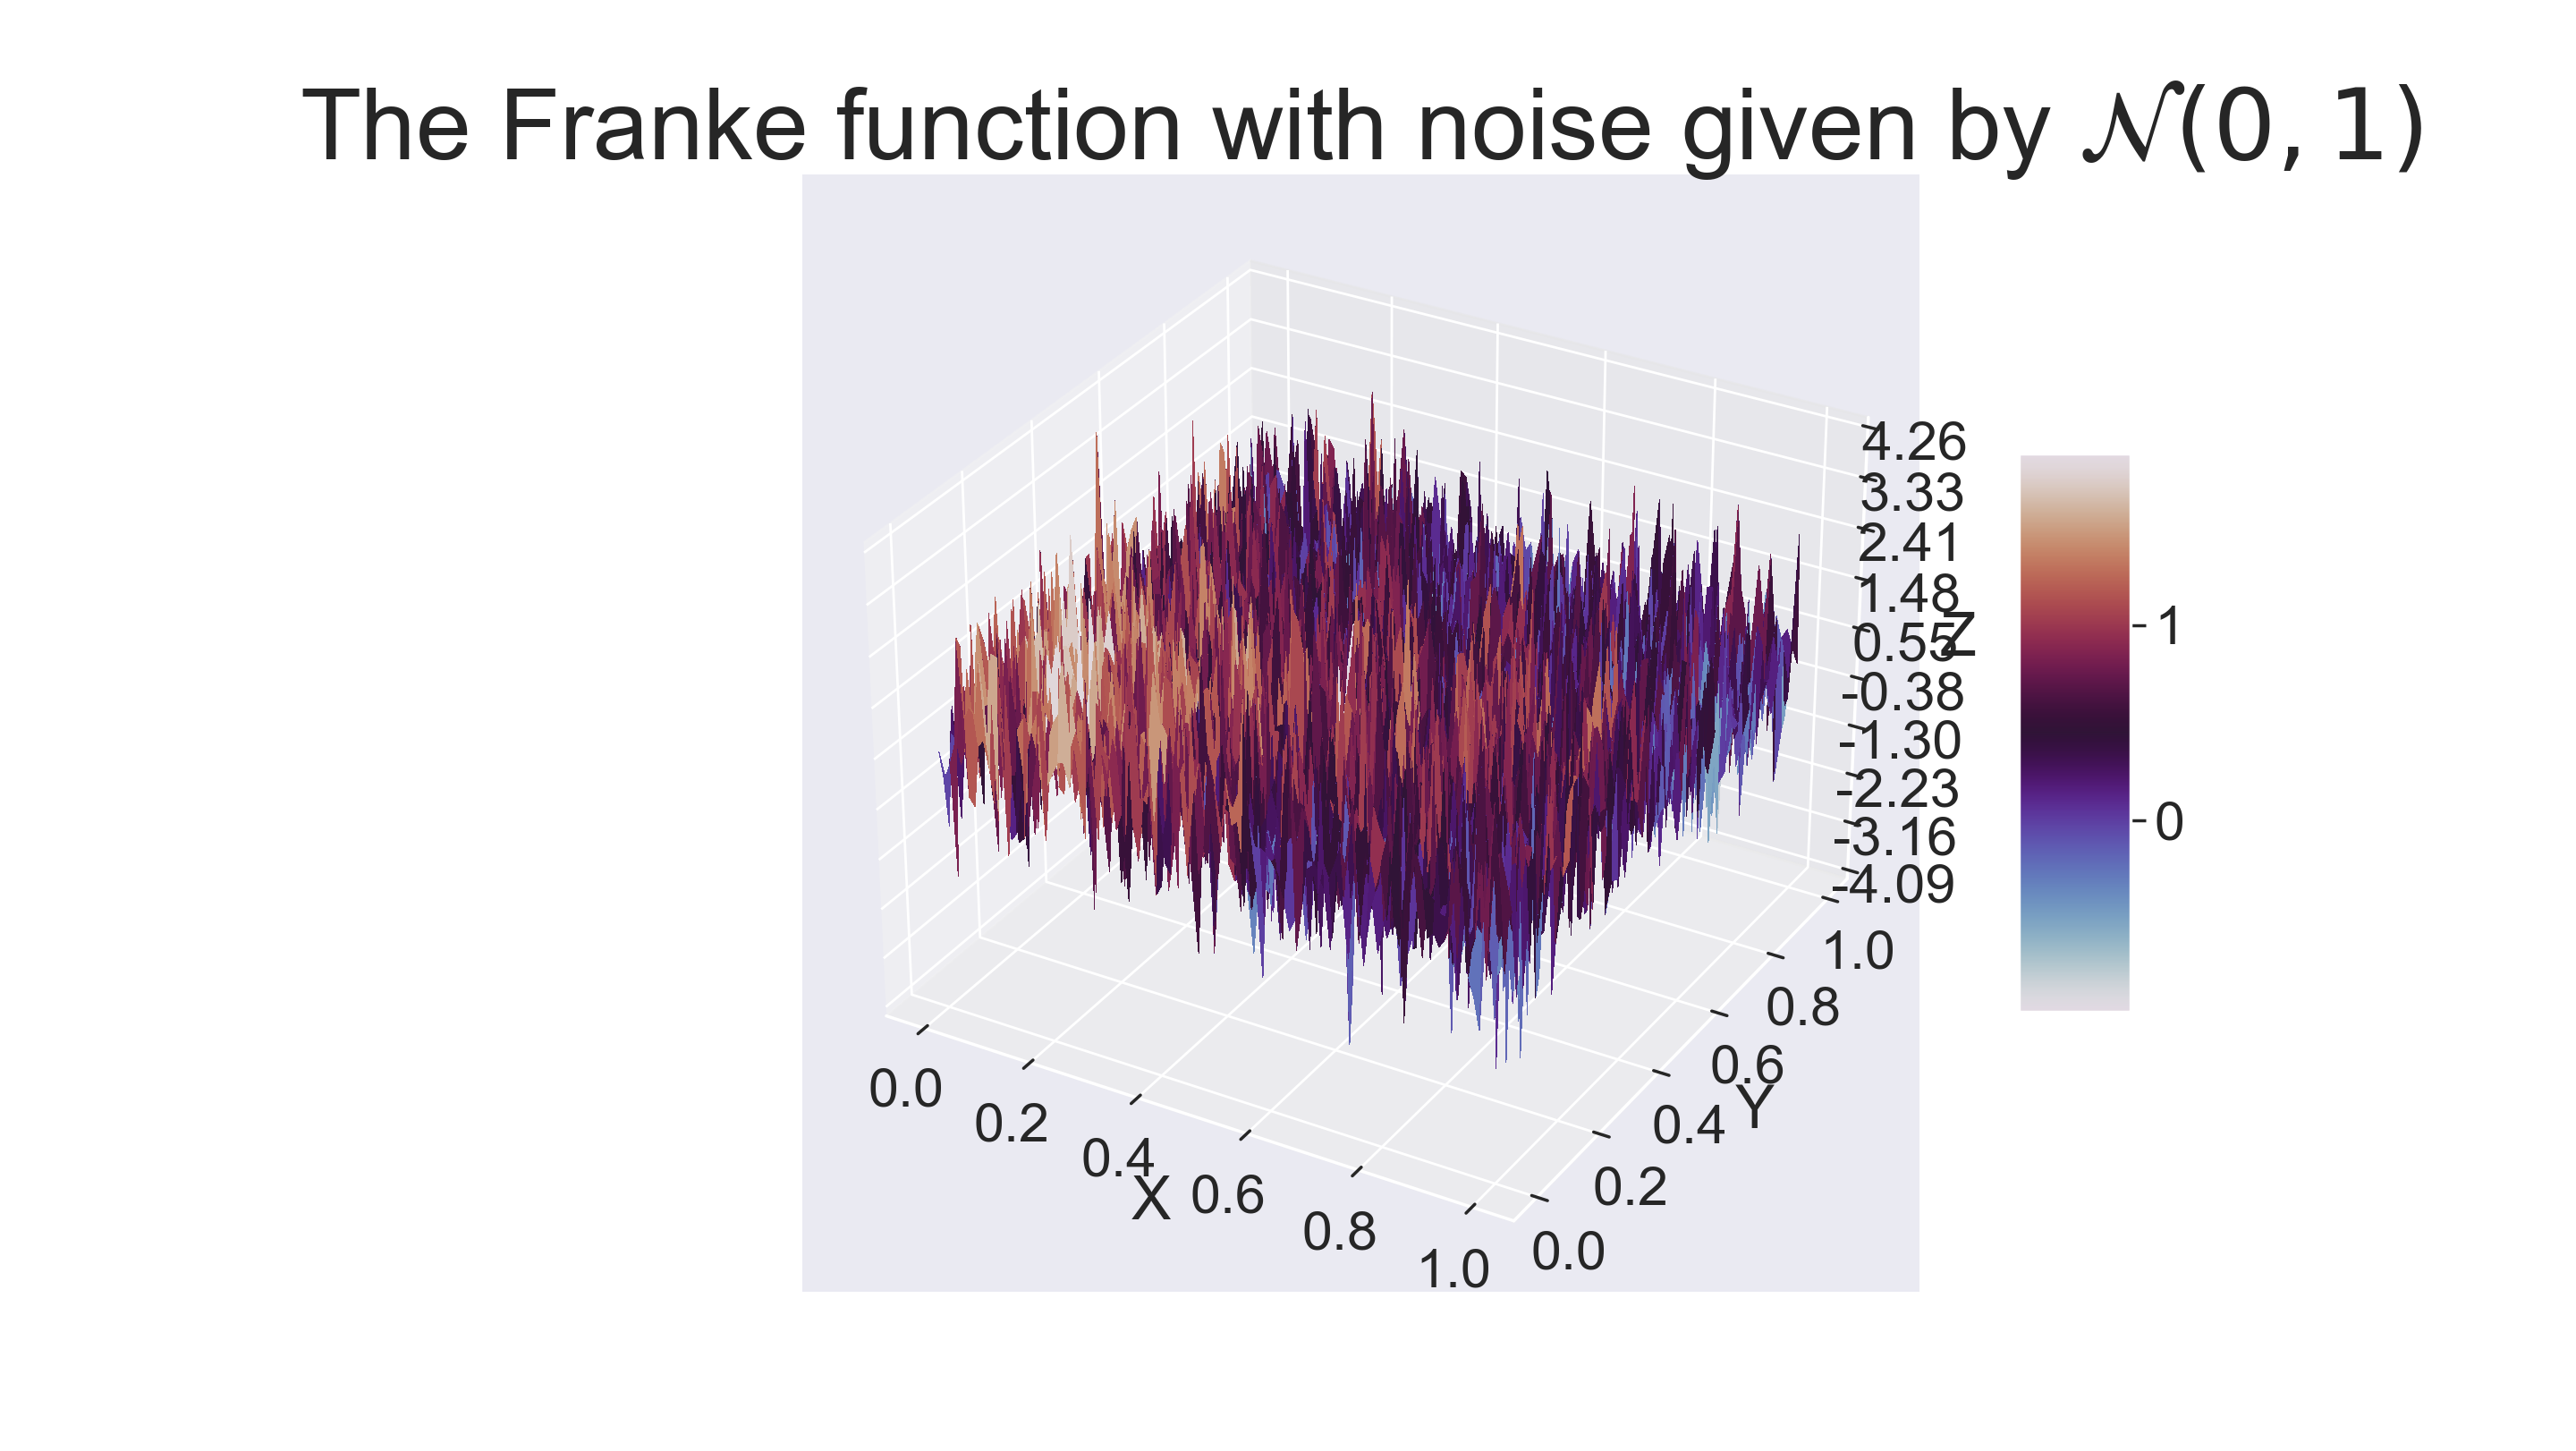
\includegraphics[width=\linewidth]{images/Figure_13.png}
	\caption{Plot showing the Franke function with noise given by the normal distribution $\mathcal{N}(0,1)$. }
	\label{franke noise 1}
\end{figure}
\noindent But if instead the normal distribution $\mathcal{N}(0,0.1)$ is 
used, the data set becomes much easier to work with, and the results becomes much prettier (as shown in figure \eqref{franke noise 0.1}) since noise has a tendency of ruining everything.
\begin{figure}[H]
	\centering
	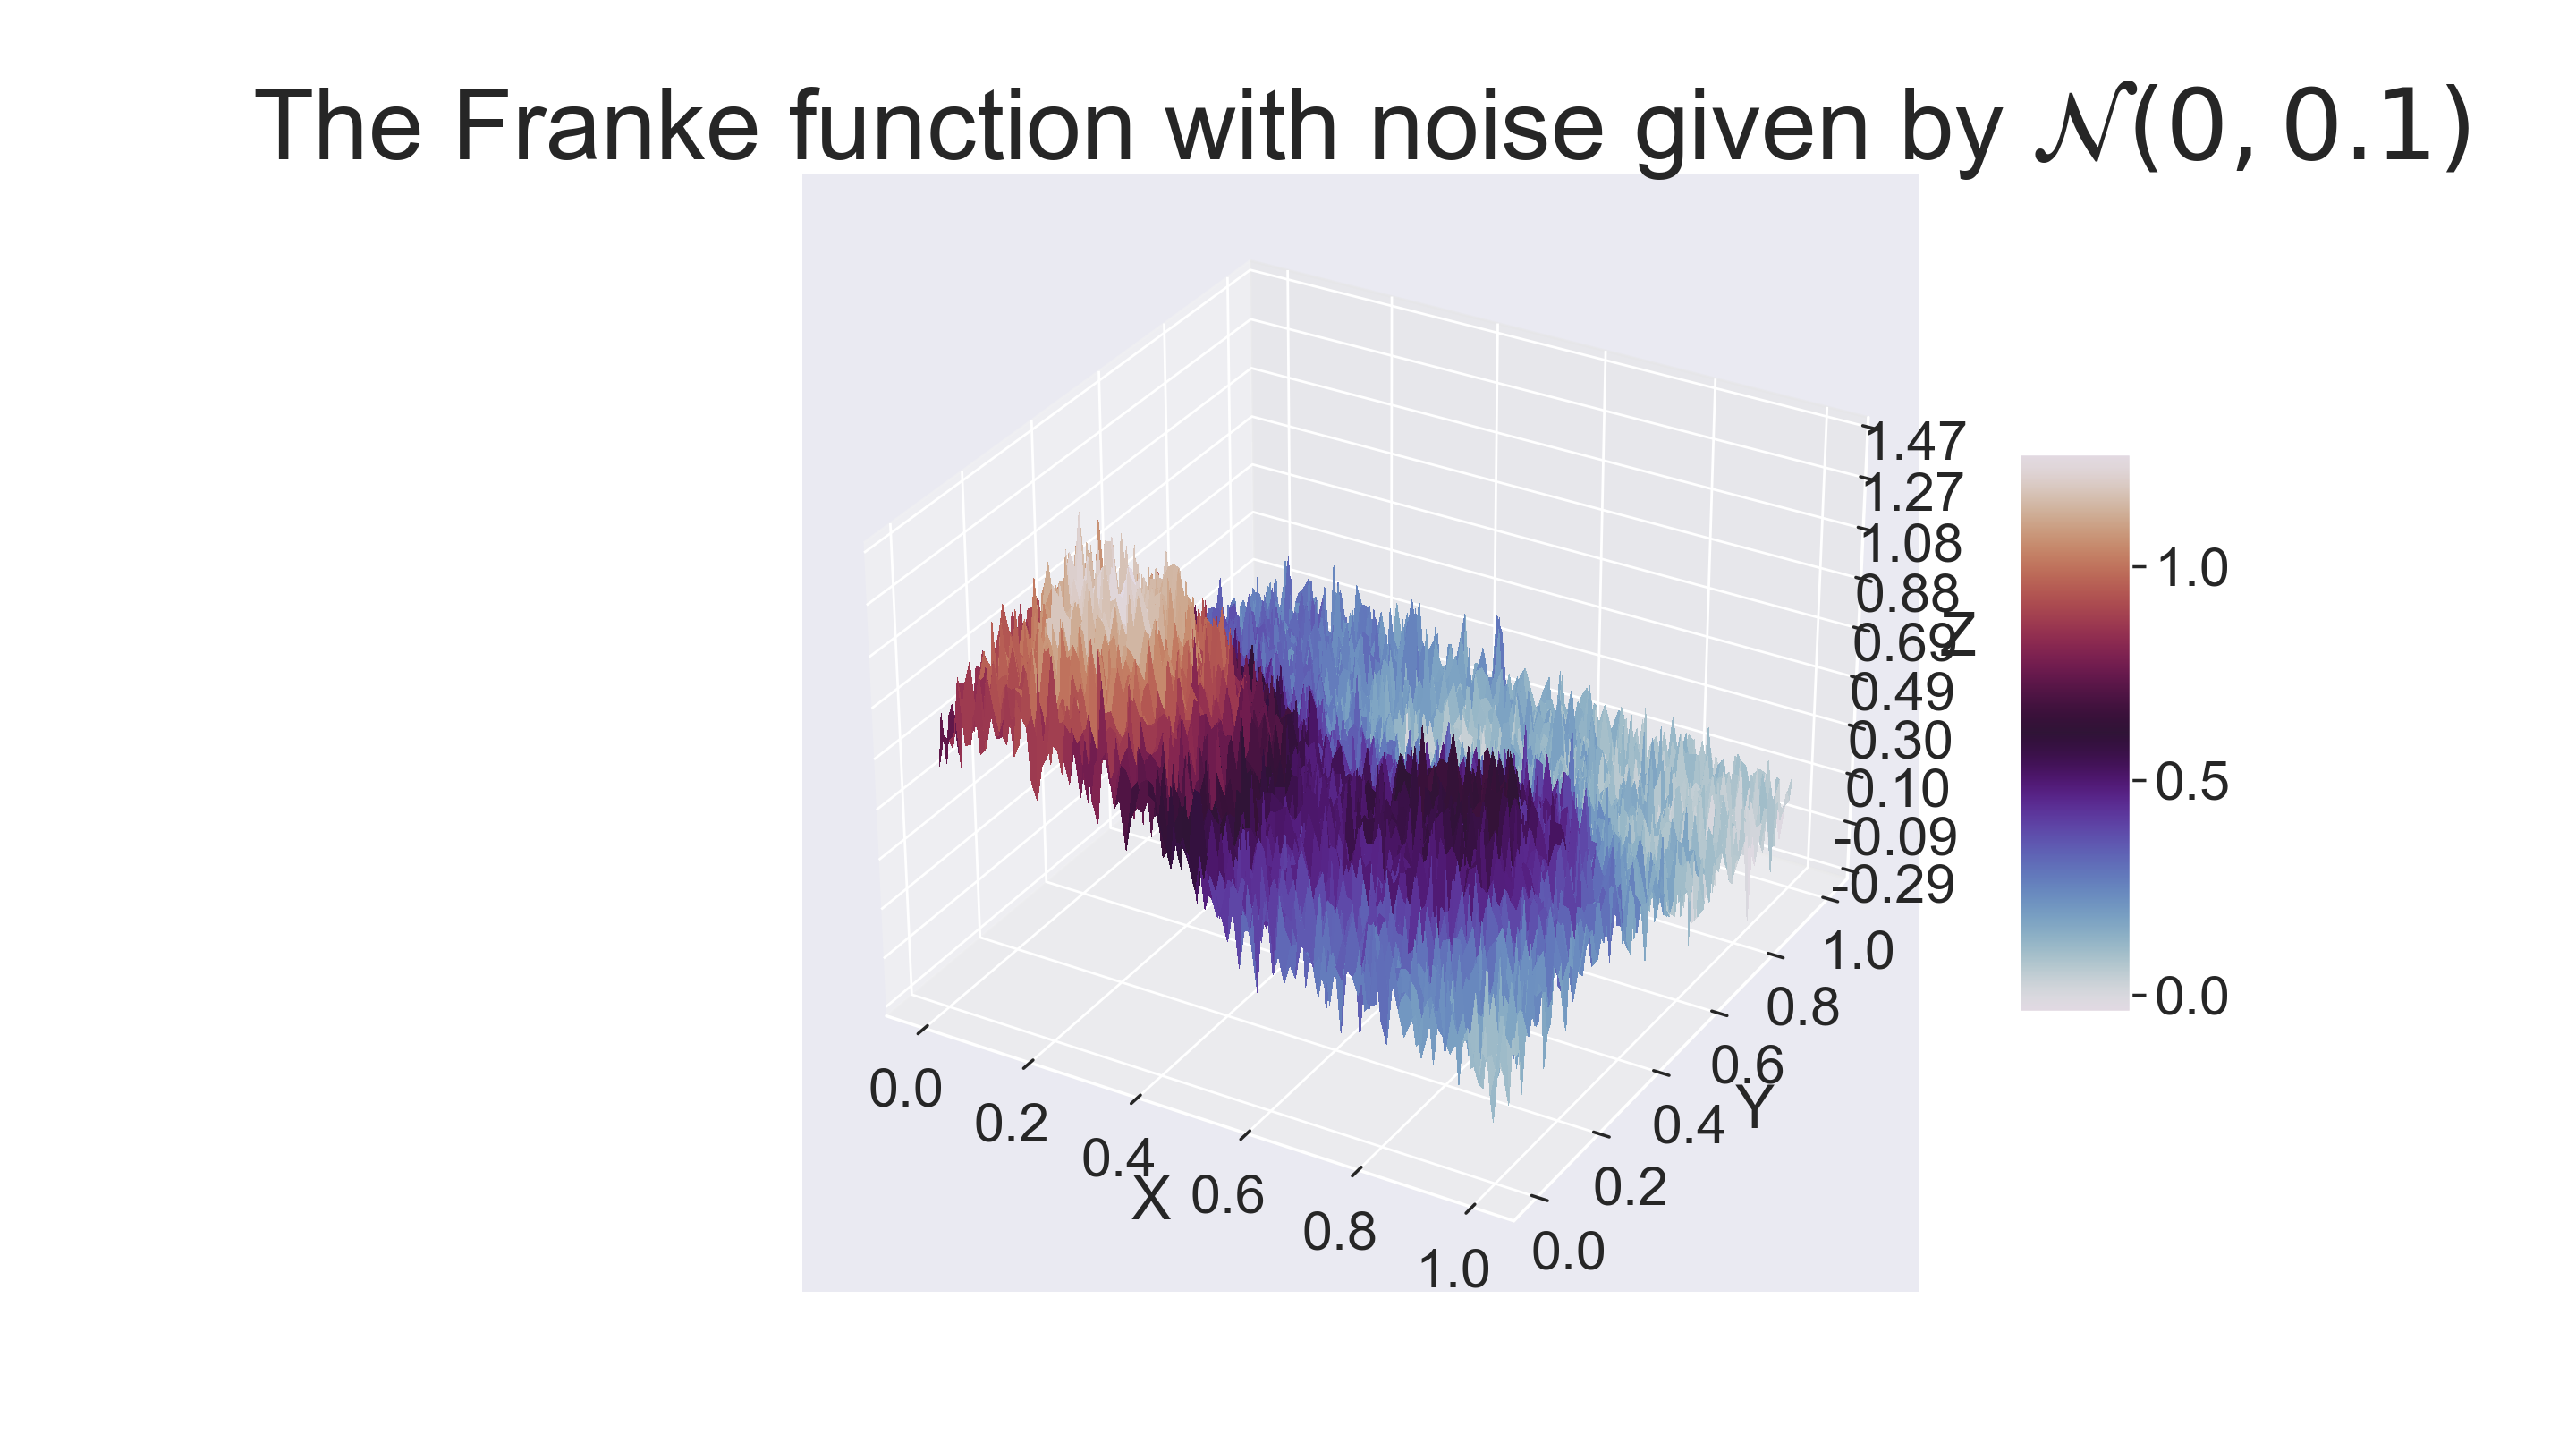
\includegraphics[width=\linewidth]{images/Figure_14.png}
	\caption{Plot showing the Franke function with noise given by the normal distribution $\mathcal{N}(0,0.1)$. }
	\label{franke noise 0.1}
\end{figure}
\noindent Now that we have gotten that out of the way, we can start actually discussing the result of the regression analysis of the Franke function.

\subsection{The Franke function}
\subsubsection{OLS}
\noindent We start with the analyses of the OLS implementation on the Franke function. It is important to note that since the parameter x and y only had values from 0 to 1 when creating the Franke function, we did not see it necessary to scale the data for any of the analysis of the Franke function, since it in a way already is scaled. The first results are the OLS model of the Franke function without noise. Figure \eqref{MSE and R2 OLS} shows the MSE and R2 scores as a function of the polynomial degree used to create the design matrix. The size of the data set analysis was a $20 \cdot 20$ matrix, were $20\%$ was put aside as test data, and the rest was used for training. What we can see from the figure is that the MSE is larger for lower polynomial degrees and starts to lower with higher values. At a fifth order polynomial degree the MSE approaches zero both for the test and training set. This is as expected, since there is no noise present there will not be any possibility for overfitting the model to the noise. Therefore the MSE will become lower and lower for higher order polynomials as shown in figure \eqref{MSE and R2 OLS}. When it comes to the R2 score we see that it becomes closer and closer to one with higher order polynomials. This is due to our model becoming increasingly better with higher orders as shown form the MSE values.

\noindent Next we look at what happens when we introduce noise given by the normal distribution $\mathcal{N}(0,0.1)$. Figure \eqref{MSE and R2 OLS noise} show the MSE and the R2 score for this case. Here we can see a classical example of overfitting the model to the noise. We see that the MSE becomes better and better for the training set but for the test set we see a sudden increase after fitting with a fourth order polynomial. This is due to the amount of data points in the different data sets, since the test data set only have $20\%$ of the original data while the training set consist of the remaining $80\%$. If we increase the number of data points the predicted model for the test data will converge towards that of the training model. 
\noindent From figure \eqref{MSE and R2 OLS} we see that when our data set does not include noise the MSE for the training data gets lower with increase in complexity, while the R2 score gets closer and closer to 1. But when we introduce noise we see from figure \eqref{MSE and R2 OLS noise} that for our test data the MSE actually increase with higher complexity. 

\noindent Next we can look at the $\beta$ values for the OLS models. What we can see from figure \eqref{beta OLS} is that for the higher order polynomials the values for the coefficients varies a lot in value. This is due to the regression method trying to fit the function to the noise, so this is a direct effect of overfitting the function with a to high order polynomial. From figure \eqref{beta OLS} we see that the beta values start to vary at as low as a fourth order polynomial and that for a fifth order polynomial the variance start to become substantially large. This is also supported by the MSE plot shown in figure \eqref{MSE and R2 OLS noise}, where we can
see that the MSE starts to gradually increase after the third order polynomial. So we clearly start to move in to the over-fit area. 

\noindent From the bootstrap results in figure \ref{fig:bootstrap_error} we can see a decrease in MSE up to polynomial degree $7$, for both the training and test data. However, we see a increase in MSE for prediction based on test data, which indicate that the model is over-fit to the training data. When we plot bias and variance, with the test error, in figure \ref{fig:bias_variance} we can see how the error decrease when the bias decrease. In addition we see increase in error when the variance increase. A decrease in the bias of the model suggest a better fit, where we reach a level of complexity to fit the data given. We also see an increase in variance for polynomial degree $7-15$, suggesting an increase in variance when we try to explain our data with higher polynomial order than necessary.

\noindent In figure \ref{fig:bias_variance} we compare the error for the Franke function, both with and without noise, with the estimated bias and variance. What we see is that MSE of the model bias follow the error up to a polynomial degree of 3 for the model with noise, and is close in value up to degree 10. At degree 10 we can see the error is close to the variance. This is expected as the error of the model can be found by summing the bias and variance \eqref{eq:bias_variance}. At the degree where both the error and variance increase, the model has become overfitted. Meaning we are training our model using unnecessary orders of polynomial degree, resulting in predictions varying. When we compare the error with the model bias and variance for the function without noise, the relation become clearer. Here the error and variance decrease more for degrees up to 7, where the bias keep decreasing and the error and variance fluctuates, and increase from degree 12. The fluctuation in MSE for the function without noise can be due to the number of samples used being small, resulting in a small data set. However, an increase in number of data points would require higher order of model complexity to fit the data. This could be studied closer by changing seed used in generating random data points.

\noindent In figure \ref{fig:cv_kfolds} the performance of an Ordinary Least Squares (OLS) regression model across varying polynomial degrees and under different k values for k-fold cross-validation. For lower polynomial degrees (around 2 to 5), the MSE remains relatively high for all k values. This suggests that a simple linear or low-degree polynomial model may not be sufficient to capture the complexity of the data. Different k values exhibit varying performance, but they all follow a similar trend across polynomial degrees. This consistency across different k values reinforces the insights drawn about the optimal polynomial degree.

\subsubsection{Ridge}
\noindent For the Ridge regression we also have to take in to account which $\lambda$ values to use in our model. To see how this value affect out model we have plotted a heat map were the MSE is plotted as a function of both different $\lambda$ values and complexity. In figure \eqref{heatmap training ridge} we see the heat map of the MSE for the training data set. From this figure we can see that for low $\lambda$ values ($\lambda<1$) the MSE is a bit below 4 which is a better result than what we got from OLS. We also see that if we increase $\lambda$ the MSE also starts to increase to about 10 for $\lambda= 10^{2}$. If we now look at a plot of how the MSE changes as a function of complexity when $\lambda=10^{-5}$ and $\lambda = 0$, so what we do is basically compere Ridge regression done with a low $\lambda$ value and OLS. We see from figure \eqref{Ridge vs OLS} that The MSE error for models fitted with polynomial of degree $0,1,2,3$ and $4$ its the same but for a model fitted with a polynomial degree of 5 the MSE is lower for Ridge regression than for OLS. This is as we expect since the extra term in the calculation for the coefficient in Ridge will try to stop the beta values from varying a lot. We can see this is the case if we look at figure \eqref{beta Ridge} were we still see that the $\beta$ values for a fit with a fifth order polynomial still varies a lot compered to lower complexity's, but it is a fair bit lower than that of OLS regression. From this we can see that if $\lambda$ is chosen correctly the model from Ridge regression is slightly better then that of OLS.

\noindent In our analysis with Ridge regression in Figure \eqref{Ridge_crossval_mse_deg}, our primary objective was to understand the model's behavior concerning varying polynomial degrees and different regularization parameters. We employed bootstrap re-sampling and cross-validation to ensure robust model evaluation and to minimize the bias-variance trade-off.

\noindent The plot showcases the model's Mean Squared Error (MSE) as a function of polynomial degrees ranging from 1 to 15. We experimented with various $\lambda$ values to discern the impact of different regularization levels. Polynomial degree denotes model complexity. As it increases, the model becomes capable of capturing intricate data patterns, but at the risk of overfitting. Our results highlight this delicate balance. At lower degrees, irrespective of regularization, the model tends to under perform, likely underfitting the data. However, for degrees between 6 to 10, a noticeable dip in the MSE is observed for certain $\lambda$ values, suggesting an optimal complexity for this data set. These insights underscore the importance of judiciously selecting the model's complexity and regularization strength to ensure balanced and optimal performance.

\subsubsection{LASSO}
\noindent For LASSO regression, we did a similar analysis to that of ridge regression. The heat maps (Figure \eqref{heat map test LASSO} and \eqref{heat map training LASSO}) shows the Mean Squared Error (MSE) as a function of different $\lambda$ values and complexity's, illustrating how the $\lambda$ value affects our model. These heat maps demonstrate that a low $\lambda$ value ($\lambda < 0.1$) and a high complexity yield a better result than a high $\lambda$ value ($\lambda > 0.1$) and a low complexity. The optimal MSE result in the heat maps occurs for $\lambda = 10^{-8}$ and degree 4, after which it gradually worsens for higher $\lambda$ values and lower complexity's until reaching $\lambda = 10^{1}$ and degree 0. In comparison to the heat maps generated for Ridge regression, the complexity appears to have significantly bigger impact on the MSE results for LASSO regression than for Ridge regression.
\noindent If we examine the line map for MSE and $R^2$ without noise (figure \eqref{MSE_and_R2_Lasso_no_noise}), we observe that LASSO with a $\lambda$ value of $10^{-5}$ produces nearly identical results to the Ridge regression and OLS. However, if we look at figure \eqref{OLS_Ridge_and_Lasso} where we plot the OLS, Ridge and LASSO when noise is added we see that the MSE for LASSO is generally allot worse compared to the two others. 
\noindent The differences between Ridge and LASSO regressions can most likely be attributed to the limited number of iterations employed. LASSO regression runs with only a small number of iterations because of the long run time. The small amount of iterations may therefore lead to a bigger tolerance that we converge against. With more iterations added, we may have achieved a better MSE for LASSO regression. From this we can see that with noise added to he Franke function, LASSO regression performs poorly compared to Ridge regression and OLS. 

\noindent In our exploration using LASSO regression, we are looking at the relationship between the model's behavior, polynomial degrees, and varying levels of the regularization parameter as denoted in Figure \eqref{Lasso_crossval_mse_deg}. Similar to our approach with Ridge regression, we employed techniques like bootstrap re-sampling and cross-validation to provide a comprehensive evaluation and to mitigate the effects of bias and variance in our model.

\noindent The depicted plot showcases the Mean Squared Error (MSE) as a function of polynomial degrees, spanning from 1 to 15, under diverse regularization strengths ($\lambda$ values). The choice of $\lambda$ in LASSO regression is critical. It not only regularizes the model but can drive certain feature coefficients to absolute zero, effectively performing feature selection.

\noindent From our results, it's evident that for extremely low regularization strengths, specifically $\lambda =10^-8$ and $\lambda=10^-6$, the MSE remains consistently high across all polynomial degrees, implying that the model may not be sufficiently regularized and might be overfitting to the training data. As we progress to moderate regularization strengths, particularly $\lambda =10^-4$ and $\lambda=10^-2$, the MSE demonstrates a dip, notably around polynomial degrees 6 to 10, suggesting these might be optimal model complexities for this data set under the given regularization. The MSE for higher regularization strengths like $\lambda =10^0$ and $\lambda=10^2$ seems to flatten out, indicating that excessive regularization might be nullifying the effect of added model complexity, leading to underfitting.

\subsection{Real terrain data}
\subsubsection{OLS}
\noindent We started by implementing OLS regression on the real terrain data. Figure \eqref{OLS terrain data} shows the MSE and R2 score as a function of complexity. As we can see from this figure the MSE is low, this is due to the way we have scaled the data set, Without proper scaling, the MSE would have been considerably higher due to the way our data set looks. Due to this scaling the result for each of out regression methods will not differ that much. What we see from figure \eqref{OLS terrain data} is as expected since the MSE decreases with complexity. As Figure \eqref{OLS terrain data} illustrates, our observations align with expectations: the MSE tends to decrease as model complexity increases. Notably, for a polynomial fit with a degree of 10, the MSE approaches zero, suggesting that a polynomial of this degree provides a accurate approximation of the true terrain data. This is again validated by looking at the R2 score, we see that when the complexity increases the R2 score begins to converge toward a value of one, which is expected when the MSE start to get closer and closer to zero. In the case with the terrain data we will continuously see that the results for our training and testing sets are almost identical, this is due to our data set being much larger than that of the Franke function, so the size although still being $20\%$ of the original data set, it includes a substantial number of data points, causing the model's performance to closely resemble that of the training set. 

For the comparison with cross validation and bootstrap we can see in Figure \eqref{fig:bootstrap_cv_terrain} that using cross validation as a re-sampling method we get a lower MSE. At lower polynomial degrees (around 2 to 4), both methods perform similarly with minimal MSE. However, as the polynomial degree increases to around 6, the MSE for bootstrap begins to rise sharply, indicating potential overfitting. In contrast, CV's MSE remains relatively stable until around degree 10, where it also exhibits a significant increase. This suggests that CV might be more robust against overfitting for intermediate polynomial degrees. At very high degrees (12-14), both methods show a pronounced spike in MSE, highlighting the dangers of over-complicating the model.

\subsubsection{Ridge}
\noindent The next part of the project was to implement Ridge regression on the terrain data. Here we started by plotting a heat map for both the training and testing data set as shown in figure \eqref{heat map Ridge Terrain data} and \eqref{heat map Ridge Terrain data test} Here we see as expected that lower $\lambda$ values and higher complexity's give a better MSE values than for lower complexity's and higher $\lambda$ values. We can also look at how the MSE and R2 score changes as a function of complexity for a $\lambda$ value equal to $10^{-5}$ as shown in figure \eqref{MSE Ridge terrain data}. Here we see a almost identical result as for OLS this has to do with the low $\lambda$ value that approaches zero. This can also indicate that there is no noise too overfit the model with in the data set since we saw from the Franke function that when no noise was present the OLS regression gave the best result but for polynomials with higher orders the model tried fitting to the noise, which may indicate that there is no substantial amount of noise present in the data set after scaling. We can further validate this by looking at the LASSO implementation. 

\noindent The Figure \eqref{fig:cv_ridge_terrain} illustrates the performance of Ridge Regression on real terrain data, evaluated using cross-validation, as a function of various polynomial degrees and regularization parameters ($\lambda$). At the lower end of the polynomial degree spectrum (around 0 to 2), the Mean Squared Error (MSE) is quite pronounced, hinting that simpler models might not adeptly represent the nuances of the terrain data.
There is a reduction in MSE as we move towards polynomial degrees of 4 to 6. This zone seems to offer a more accurate representation of the data without excessive complexity. The region around polynomial degrees of 4 to 6 combined with $\lambda$ values ranging from $10^{-5}$ to $10^{-3}$ appears to deliver the lowest MSE, marking it as a potential optimal setting for this data set.

\subsubsection{LASSO}
\noindent We then implemented the LASSO regression on the terrain data. Here we also plotted heat maps for both the training and test data shown in figure \eqref{Heat map LASSO terrain training} and \eqref{Heat map LASSO terrain testing}. The heat maps gave approximately the same results for the terrain data as for the Franke function. They demonstrate that lower $\lambda$ values and higher complexity's gives the best MSE values as expected. 

\noindent If we then examine the line map for MSE and $R^2$ score changes as a function of complexity for a $\lambda$ value equal to $10^{-5}$ shown in figure \eqref{MSE LASSO terrain data}, we see it is nearly identical to the results from the Ridge regression and OLS results. Based on the results for LASSO on the Franke function it may indicate that the similarity's between the results stem from there being little to no noise present in the terrain data set after scaling. 

\noindent If we look at figure \eqref{MSE for OLS, Ridge and LASSO} where we plot the OLS, Ridge and LASSO for the terrain data, we see that all the three methods gets better with higher complicity's, but LASSO is generally allot worse compared to the two others. The LASSO regression for the real data may also be worse because of she small amount of iterations that may lead to a bigger tolerance that we converge against.

\noindent The Figure \eqref{fig:cv_lasso_terrain} define the performance of LASSO Regression on real terrain data, evaluated with cross-validation, based on various polynomial degrees and regularization parameters ($\lambda$). At the initial polynomial degrees (around 0 to 2), the Mean Squared Error (MSE) is relatively high. This suggests that models of low complexity may not adequately encapsulate the intricacies present in the terrain data. The optimal region, in terms of minimizing MSE, appears to be around polynomial degrees of 4 to 6, paired with $\lambda$ values between $10^{-5}$ and $10^{-3}$. This suggests that within these parameter settings, the model performs best for the given data set.

%
\section{Conclusion}
\thispagestyle{plain}
\noindent To summarize our findings, it is clear that the choice of the best regression method depends on the data set used. In scenarios where the data is noise-free, OLS proves to be the most effective regression method. But noise-free data is usually not the case. What we found was that the best regression method for the Franke function with noise given by the normal distribution $\mathcal{N}(0, 0.1)$, was Ridge for higher polynomial degrees, this is due to OLS over-fitting the data to the noise for higher polynomial degrees, while Ridge and LASSO tries to minimise the variance in $\beta$ values to avoid this problem. 
Even though LASSO aims to minimize variance in $\beta$ values, it exhibited the worst performance among the three regression methods. However, it remains uncertain whether Lasso could outperform Ridge and OLS in handling noise due to limitations in iterations. The decision to restrict iterations was influenced by run time constraints, leaving the true capabilities of Lasso in this scenario unknown.
\noindent For our terrain data we surprisingly found that OLS gave the model with the lowest MSE. From what we can see in figure \eqref{OLS 3D figure terrain data} the terrain data looks a little noise, but it may be due to the scaling of the data set that makes OLS the best regression method for the terrain data. 

\noindent The improvement potential for this project is high, due to some grope problems we got started on the project late together as one group. Therefor the structure on GitHub and the cods are quite messy. This is something we will work on improving for the next project. 
% acknowledgements (optional)
\section{Acknowledgement}
\noindent We would like to thank Morten Hjorth-Jensen for his amazing and well crafted jupyter notebooks. Additionally, we would like to acknowledge the valuable 
inspiration provided by ChatGPT throughout the report-writing process. 
%
\clearpage
\newpage
\onecolumngrid
\appendix
\pagenumbering{alph}
\thispagestyle{plain}

We have assumed that our data can be described by the continous function 
$f(\boldsymbol{x})$, and an error term $\boldsymbol{\epsilon} ~ N(0, \sigma^{2})$. 
If we approximate the function with the solution derived from a model $\boldsymbol{\tilde{y}} = X\boldsymbol{\beta}$ the data can be described with $\boldsymbol{y} = X\boldsymbol{\beta} + \boldsymbol{\epsilon}$. 
The expectation value 

\begin{align*}
    %\hskip\parindent
    \mathbb{E}(\boldsymbol{y}) &= \mathbb{E}(X\boldsymbol{\beta} + \boldsymbol{\epsilon}) \\
    &= \mathbb{E}(X\boldsymbol{\beta}) + \mathbb{E}(\boldsymbol{\epsilon}) && \text{where the expected value $\boldsymbol{\epsilon} = 0$} \\
    \mathbb{E}(y_{i}) &= \sum_{j=0}^{P-1} X_{i,j} \beta_{j} && \text{for the each element} \\
    &= X_{i,*} \beta_{i} && \text{where $_{*}$ replace the sum over index $i$} \\
\end{align*}


The variance for the element $y_{i}$ can be found by
\begin{align*}
    \mathbb{V}(y_{i}) &= \mathbb{E} \big[ (y_{i} - \mathbb{E}(y_{i}))^{2} \big] \\
    &= \mathbb{E} (y_{i}^{2}) - (\mathbb{E}(y_{i})^{2}) \\
    &= \mathbb{E} ((X_{i,*} \beta_{i} + \epsilon_{i})^{2}) - (X_{i,*} \beta_{i})^{2} \\
    &= \mathbb{E} ((X_{i,*} \beta_{i})^{2} + 2\epsilon_{i}X_{i,*} \beta_{i} + \epsilon^{2}) - (X_{i,*} \beta_{i})^{2} \\
    &= \mathbb{E} ((X_{i,*} \beta_{i})^{2}) + \mathbb{E} (2\epsilon_{i}X_{i,*} \beta_{i}) + \mathbb{E} (\epsilon^{2}) - (X_{i,*} \beta_{i})^{2} \\
    &= (X_{i,*} \beta_{i})^{2} + \mathbb{E} (\epsilon^{2}) - (X_{i,*} \beta_{i})^{2} \\
    &= \mathbb{E} (\epsilon^{2}) = \sigma^{2} \\
\end{align*}

The expression for the optimal parameter 
\begin{align*}
    \boldsymbol{\hat{\beta}} &= (\boldsymbol{X}^{T} \boldsymbol{X})^{-1} \boldsymbol{X}^{T} \boldsymbol{y} \\
\end{align*}
We find the expected value of $\boldsymbol{\hat{\beta}}$
\begin{align*}
    \mathbb{E}(\boldsymbol{\hat{\beta}}) &= \mathbb{E}((\boldsymbol{X}^{T} \boldsymbol{X})^{-1} \boldsymbol{X}^{T} \boldsymbol{y}) \\
    &= (\boldsymbol{X}^{T} \boldsymbol{X})^{-1} \boldsymbol{X}^{T} \mathbb{E}(\boldsymbol{y}) && \text{using that $\boldsymbol{X}$ is a non-stochastic variable} \\
    &= (\boldsymbol{X}^{T} \boldsymbol{X})^{-1} \boldsymbol{X}^{T} \boldsymbol{X} \boldsymbol{\beta} && \text{using $\mathbb{E}(\boldsymbol{y}) = \boldsymbol{X} \boldsymbol{\beta}$} \\
    &= \boldsymbol{\beta} \\
\end{align*}
we can find the variance by 
\begin{align*}
    \mathbb{V}(\boldsymbol{\hat{\beta}}) &= \mathbb{E} \big[ (\boldsymbol{\hat{\beta}} - \mathbb{E}(\boldsymbol{\hat{\beta}}))^{2} \big] \\
    &= \mathbb{E} (\boldsymbol{\hat{\beta}} \boldsymbol{\hat{\beta}}^{T}) - \mathbb{E}(\boldsymbol{\hat{\beta}})^{2}  \\
    &= \mathbb{E} (((\boldsymbol{X}^{T} \boldsymbol{X})^{-1} \boldsymbol{X}^{T} \boldsymbol{y}) ((\boldsymbol{X}^{T} \boldsymbol{X})^{-1} \boldsymbol{X}^{T} \boldsymbol{y})^{T}) - \boldsymbol{\hat{\beta}}\boldsymbol{\hat{\beta}}^{T}  \\
    &= \mathbb{E} ((\boldsymbol{X}^{T} \boldsymbol{X})^{-1} \boldsymbol{X}^{T} \boldsymbol{y} \boldsymbol{y}^{T} \boldsymbol{X} (\boldsymbol{X}^{T} \boldsymbol{X})^{-1}) - \boldsymbol{\hat{\beta}}\boldsymbol{\hat{\beta}}^{T}  \\
    &= (\boldsymbol{X}^{T} \boldsymbol{X})^{-1} \boldsymbol{X}^{T} \mathbb{E} (\boldsymbol{y} \boldsymbol{y}^{T}) \boldsymbol{X} (\boldsymbol{X}^{T} \boldsymbol{X})^{-1} - \boldsymbol{\hat{\beta}}\boldsymbol{\hat{\beta}}^{T}  \\
    &= (\boldsymbol{X}^{T} \boldsymbol{X})^{-1} \boldsymbol{X}^{T} (\boldsymbol{X} \boldsymbol{\beta} \boldsymbol{\beta}^{T} \boldsymbol{X}^{T} + \sigma^{2}) \boldsymbol{X} (\boldsymbol{X}^{T} \boldsymbol{X})^{-1} - \boldsymbol{\hat{\beta}}\boldsymbol{\hat{\beta}}^{T}  \\
    &= \boldsymbol{\beta} \boldsymbol{\beta}^{T} + \sigma^{2}((\boldsymbol{X}^{T} \boldsymbol{X})^{-1} \boldsymbol{X}^{T} \boldsymbol{X} (\boldsymbol{X}^{T} \boldsymbol{X})^{-1}) - \boldsymbol{\hat{\beta}}\boldsymbol{\hat{\beta}}^{T}  \\
    &= \sigma^{2}(\boldsymbol{X}^{T} \boldsymbol{X})^{-1} \\
\end{align*}
%
\newpage
\clearpage
%
\section*{References}  % the asterisk (*) after \section makes the section numbering go away
\bibliography{references/citation}


\end{document}
